
\documentclass[a4paper ]{article}

\usepackage{etex}		% clash when too many dimensions
\usepackage{lettrine}	% für ersten Buchstaben groß

\usepackage[english]{babel}
\usepackage[utf8x]{inputenc}
\usepackage{amsmath}
\usepackage{graphicx}
%PATH MAC
%\graphicspath{{/Users/marcfabel/Dropbox/Uni/Tinbergen/MPhil/STATA/GRAPHS/}}


%PATH Windows
%\graphicspath{{C:/Users/fabel/Dropbox/Uni/Tinbergen/MPhil/STATA/graphs/}}


%\usepackage[colorinlistoftodos]{todonotes}
\usepackage{ amssymb }
\usepackage{amsmath}
\usepackage{parskip}
\setlength{\parindent}{0pt}
\DeclareGraphicsExtensions{.pdf,.png,.jpg}
\usepackage{booktabs}
\usepackage{longtable}
\usepackage{enumerate} % roman enumeration
\usepackage{wrapfig}

\usepackage[labelfont=bf,labelsep = period, singlelinecheck=off,justification=raggedright]{caption}%both together help to have subfigures, other specifications which are nice: labelformat = parens -> number in paranthesis
\usepackage[singlelinecheck=on]{subcaption}

%\usepackage{tikz}
%\usetikzlibrary{decorations.pathreplacing}

\usepackage[authoryear, round, comma]{natbib}

\usepackage{titlesec} %section headers 
\titleformat*{\section}{\large\bfseries}



\usepackage{dsfont} %Double stroke, e.g. for indicator function


\usepackage{afterpage}
\usepackage{lscape}
\usepackage{multirow}
\usepackage{adjustbox}

\usepackage[hyphens]{url}



\usepackage[usenames,dvipsnames,svgnames,table]{xcolor}
\definecolor{darkblue}{rgb}{0.0,0.0,0.6}

 \usepackage{hyperref}
 \hypersetup{
      colorlinks   = true,
     citecolor    = darkblue,
 	linkcolor= darkblue,
     urlcolor=darkblue }

\usepackage[
	top    = 4.3cm,
	bottom = 4cm,
	left   = 3.8cm,
	right  = 3.8cm]{geometry}		%option: showframe=true (see page boundaries)
	
\usepackage{changepage} % adjust width on sides of the page, needed tto place tables in the middle of the page





\usepackage{pdflscape}
\usepackage{layouts}% temporär, zurbestimmung von textwdith

\usepackage{fancyhdr}
\pagestyle{fancy}
\fancyhf{}
%\chead{MATERNITY LEAVE AND LONG-RUN HEALTH OUTCOMES}
\chead{Maternity leave and long-run child health}
\rhead{\thepage}
\renewcommand{\headrulewidth}{0.5pt}




%HEADER EINSTELLEN:
\newlength\FHoffset
\setlength\FHoffset{0cm} % definiert Anzahl der cm, die der Header überlappt-muss zu (NEW)Geometry passen
\addtolength\headwidth{2\FHoffset}

\newlength\FHleft
\newlength\FHright

% here the trimmings are controlled by the user
\setlength\FHleft{1cm}
\setlength\FHright{1cm}
%Quelle: http://tex.stackexchange.com/questions/55981/headrule-length-in-fancyhdr


\usepackage{supertabular}






\title{Maternity Leave Coverage and the Long-Term Health Outcomes of Children in Germany%\footnote{We are grateful to Eva Degler, Ingrid H\"agele, Theresa Huck, Maarten Lindeboom, Erik Plug and participants of the Tinbergen Institute MPhil Thesis workshop for helpful comments and suggestions. All remaining errors are our own.}
}
\author{{\color{red}Preliminary and incomplete draft: Please do not cite or circulate}\\ \\
Natalia Danzer \& Marc Fabel \thanks{Marc Fabel (corresponding author): Munich Graduate School of Economics (MGSE) and Ifo Institute (email: \href{mailto:fabel@ifo.de}{fabel@ifo.de}).\newline Natalia Danzer: Ifo Institute, University of Munich and IZA (email: \href{mailto:danzer@ifo.de }{danzer@ifo.de }).}}
\date{April 2018}


\begin{document}


\thispagestyle{empty}\fancyhf{}
\chead{Maternity leave and long-run child health}
\rhead{}
\renewcommand{\headrulewidth}{0.5pt}



%

\newpage

\clearpage
\setcounter{page}{1}    
\rhead{\thepage}

        \newpage

\renewcommand{\abstractname}{\vspace{-\baselineskip}}	% GET RID OF ABSTRACT TITLE
\maketitle
    \begin{abstract}\noindent 
   \footnotesize{\begin{center}\textbf{Abstract}\end{center}
   Over the past decades, parental leave mandates have witnessed a considerable boost in many developed countries. The average length of parental leave across OECD countries increased from 15 to 63 weeks between 1970 and 2015. While previous literature is inconclusive about long-run impacts of parental leave on children's educational attainment and labor market outcomes, long-run health effects remain unknown. Therefore, we evaluate the impact of an expansion in maternity leave coverage from two to six months on children's long-term health outcomes in Germany. We combine a regression discontinuity with a difference-in-difference approach in order to estimate a causal effect: health outcomes of children who were born shortly before and after the implementation of a policy reform are compared to the outcomes of children who were born in the same calendar months but in a year in which no legislative change occurred. Subsequently, we apply a life-course approach, investigate heterogeneous intention-to-treat effects and explore potential mechanisms through which the reform affected long-run health outcomes. By using 21 waves from the German Socio-Economic Panel (SOEP), we obtain first results that suggest a negative effect of the length of maternity leave on several measures of subjective health. In contrast, little evidence supports the hypothesis that the length of maternity leave affects children's objective or biometric health outcomes.\newline\\ {\color{red}Currently, we are extending the analysis by applying the same identification strategy to other datasets. For that purpose, we use the German Micro Census, Europe's largest household survey, and hospital administrative data, which contains detailed information about all inpatients' socio-demographic characteristics, diagnoses, and treatment in Germany over the past 19 years.} \\\newline \textbf{Keywords:} Early childhood development, health, paid maternity leave, regression discontinuity and difference-in-differences, life-cycle approach \newline \textbf{JEL codes:} I10, J13, J18}
    \end{abstract}
   
   
   
    %This paper assesses the impact of the length of maternity leave on children’s long-run health outcomes. Our quasi-experimental design evaluates an expansion in maternity leave coverage from two to six months, which occurred in the Federal Republic of Germany in 1979. The expansion came into effect after a sharp cutoff date and significantly increased the time working mothers stayed at home with their newborns. In our analysis, we exploit the German Micro Census and hospital registry data, containing detailed information about the universe of inpatients' diagnoses and treatment for the years 1995 to 2014. By tracking the health of treated and control children from age 16 up to age 35, we provide new insights into the trajectory of health differentials over the life-cycle.
%We find a positive effect of the legislative change on several measures of long-term child health. Our intention-to-treat estimates suggest that children who were born shortly after the implementation of the reform experience fewer hospital admissions and are less likely to be diagnosed with mental and behavioral disorders.  
%

    

%\renewcommand\thesection{\arabic{section}.}
%\renewcommand\thesubsection{\thesection.\arabic{subsection}}


%\renewcommand\thesection{\Roman{section}}
%\renewcommand\thesubsection{\thesection.\arabic{subsection}}


\newpage

%-----------------------------------------------------------------------------------------------------------------------------------
%	INTRODUCTION
%-----------------------------------------------------------------------------------------------------------------------------------
\section{Introduction}
%EINLEITENDER ABSATZ
\lettrine[lines=2]{\color{gray}\textbf{F}}{ }emale labor force participation (LFP) rates have increased considerably across the western hemisphere over the last decades. The average female LFP rate across all OECD countries raised from 47.6\% in 1970 to 63\% in 2015. This can be partly explained by the promotion of parental leave legislation, as especially mothers of young children are among the groups which denoted the highest increase in LFP rates. Figure \ref{fig:PLOECD} shows that both female labor force participation and the length of parental leave schemes have witnessed a substantial boost within the last 45 years. Next to encouraging female employment the policies intend to encourage fertility, advocate gender equality and most importantly safeguard the well-being of mother and child.\newline Parental leave policies are designed to protect against job dismissal, prevent damages to the health of mother or child and secure standards of living by compensating income losses. Parents are given the possibility to take a break from work and focus on child care. This is based on the insight that the first year in a child's life is essential for subsequent child development (see for instance \cite{flavell1993cognitive}). \newline The German Federal Ministry of Family Affairs is willing to spend a great deal of money for achieving these social goals and is expected to pay six billion euros for parental leave in 2016. This amount equals two third of the ministry's budget and corresponds to almost 2\% of the entire 2016 federal government budget.\footnote{Compare with: "Gesetz über die Feststellung des Bundeshaushaltsplans für das Haushaltjahr 2016" (Budget act), Bundesgesetzblatt (Federal law gazette), Part I, Nr. 54, p. 2378-2398, 28.12.2015.} With such great transfer payments involved, there is an intrinsic desire to evaluate whether the financial efforts pay off. The aim of this article is to investigate the effects of the length of parental leave on children's health in the long-run. \newline

%MECHANISMS
The idea that parent's decision to postpone their return to work may lead to changes in children's long-run health is based on the following empirical facts. First, mothers who abstain from work longer are more likely to breastfeed and do so for a longer period \citep{berger2005maternity}. The associated benefits of breastfeeding are numerous and include all kind of positive health effects for the child \citep{horta2007evidence}. Second, without adequate financial support it is likely that there are changes in household income, because one parent is staying at home taking care of the infant instead of working. It is presumed that lower levels of household income have direct consequences for the health of the child (see e.g. \cite{case2002economic} and \cite{hoynes2015income}). Third, the additional time, which parents spend with their offspring, helps to strengthen parent-child linkages. These relationships are crucial for the expansion of cognitive skills \citep{klaus1998mother}. Thus, parental leave helps to foster child development, which has the potential to affect adulthood labor market, education, family and health outcomes \citep{currie2011human}.\newline

%WHY IS GERMAN REFORM SO GOOD
This article examines the effect of maternity leave on children's long-run health outcomes in the context of a reform that occurred in the Federal Republic of Germany in 1979, in which the length of maternity leave was increased from two to six months. The reform is for a number of reasons well suited to investigate the impact of the length of maternity leave on children's health. First, the reform provides exogenous variation in maternity leave as the eligibility for the more generous leave scheme is contingent on the child's date of birth. Therefore, it is possible to estimate a causal effect by comparing health outcomes of children born before and after the threshold. Furthermore, children who are born in the same months around the cutoff but in years in which no policy change happened are included into the analysis to have an additional comparison group. Thus, this approach combines a pure regression discontinuity with a difference-in-difference design (DD-RD).
Second, the reform was announced shortly before it took effect. Therefore, anticipation effects (the children were already conceived at the time of announcement) are negligible and an endogenous selection into the more generous scheme seems unlikely. 
Third, the reform stretches further back in the past than many other comparable reforms. This allows a better identification as more evidence has already accumulated. Additionally, due to the design of the reform that increases maternity leave from two to six months, it is possible  to examine a particularly crucial time period for a child's development.  \newline

%DATA AND RESULTS
For the empirical investigation we use the German Socio-Economic Panel (SOEP), which contains a broad range of health variables that are recorded over the period 1993-2014.\footnote{Currently, we extend this analysis by using data from the German Micro Census, Europe's largest household survey, and hospital administrative data, which contains detailed information about all inpatients' socio-demographic characteristics, diagnoses and treatment in Germany over the past 19 years. The new datasets help to considerably increase the number of estimations for the estimation. }
The main results can be summarized as follows. We find little evidence for the hypothesis that the length of maternity leave positively affects children's health outcomes. In contrast, the results suggest quite the opposite. The DD-RD design shows that extending the length of the maternity leave from two to six months increased the number of doctor consultations and sick days as well as the likelihood of suffering from a chronic disease over the whole period (1993-2014). Children born under the new regime have a worse perception of their health status as well as more concerns about their health, they have more problems to carry out daily activities and they are more often socially constrained. Finally, respondents are more likely to smoke - both at the extensive and intensive margin - and sleep less in response to the reform. Applying a life-course perspective reveals that the effects are not only driven by either medium- or long-term effects. The conclusions from a heterogeneity analysis of the causal effects show that the effects of the reform are worse for men, respondents with no children, people who have a household income below the median and whose parents have a school certificate from the lowest track. Interestingly, people with a school certificate from the Gymnasium (the highest track) report a worse self-assessed health status in response to the reform, which is in line with research about reporting errors. This indicates that better educated individuals tend to report their health more accurately \citep{cawley2015health}. A spatial investigation adds to the impression that the socioeconomic situation (either by the parents or the general level of the federal state) is crucial for the success of parental leave laws. We also examine potential mechanisms through which the reform in maternity leave may affect adulthood health outcomes. We find no evidence that the reform has an effect on educational attainment, but it reduces the likelihood of being employed. Moreover, there is limited evidence that the expansion in maternity leave led to a decline in household income as well as the probability of being married and having children.\newline

%PREVIOUS LITERATURE
This article is related to previous literature in the following ways. First, it relates to the emerging literature about early childhood influences on later life outcomes. \cite{currie2011human} offer a very detailed summary of recent work in that strand of research. They argue that experiences made within the first five years have important and persistent explanatory power for adulthood outcomes. The nature of influences that have long-term consequences can be numerous and range from variation in household income to toxic exposure. As this article investigates the effect of maternity leave on children's health outcomes the context is set on early childhood influences in the home environment. Although the nature of influences are quite diverse across studies, the focus on human capital accumulation and labor market outcomes as children's long-term outcomes is often very similar. For instance, \cite{carneiro2015flying} investigate the impact of a similar reform as this paper but use a reform in Norway. They find that a change from a three month long unpaid - to a four month paid leave decreased the likelihood to drop-out from high school and increased earnings of individuals when aged 30. \cite{rasmussen2010increasing} uses a reform in Denmark in which parental leave was increased from 14 to 20 weeks. Contrary to the previous study, she does not find any measurable impact of the reform on children's long-term educational outcomes. The inconclusiveness is characteristic for this strand of research, which is one motivation for this paper. By investigating health outcomes in the long-run, we hope to provide additional evidence for the importance of early life influences for another set of outcomes, which has not been in the center of research so far. \newline
Second, the article is also related to the literature about the impact of parental leave on health. There is evidence that parental leave may affect the health of the child and the parents. Both \cite{stearns2015effects} and \cite{rossin2011effects} use data from the US and show that maternity leave is positively associated with infant health outcomes. They find that maternity leave led to a reduced likelihood of early term birth and increases in birth weight, which can be regarded as a key indicator of health of newborns and has high predictive power for future outcomes \citep{almond2005costs,currie2007biology}. \cite{beuchert2014length} use an expansionary reform of maternity leave in Denmark to investigate the impacts on health outcomes of mothers and child. They find that the expansion in maternity leave had only limited effects on women's hospital admission rates in the short-run and no effect on the probability of receiving antidepressants.\footnote{Other relevant studies in that field are \cite{avendano2015long} and \cite{chatterji2005does}.} Most of the literature on the impact of maternity leave on health outcomes focuses on short-run effects. We extend this literature by considering impacts of maternity leave on health outcomes decades later.\newline 

%EXTENSION OF LITERATURE
The empirical analysis in this paper expands and clarifies previous literature on several dimensions. First, the article evaluates long-run health outcomes, while the literature either focused on short-run health outcomes (such as \cite{stearns2015effects} and \cite{rossin2011effects}) or long-run educational attainment or labor market outcomes (e.g. \cite{carneiro2015flying} and \cite{rasmussen2010increasing}). Second, the data allows to look at an unusual broad range of health outcomes observed over a long period of time (maximum 21 years of adulthood). Third, we apply a life-course perspective in a complete new setting. \cite{garrouste2015lasting} use this approach in order to examine whether there are changes in long-run health in response to leaving school in a bust. Finally, with the identification strategies at hand there is less dependence on identifying assumptions than in other studies \citep{ruhm2000parental}. \newline

The remainder of the article proceeds as follows. The next section outlines mechanisms through which the expansion in maternity leave could affect children's health outcomes in adulthood. Additionally, we discuss background information about maternity leave and benefit legislation in Germany during the late 1970s. Section \ref{sec: ident.strategy} summarizes the applied identification strategies. Data and variables are described in Section \ref{sec: Data}. Section \ref{sec: Results} reports results and Section \ref{sec: Conclusion} presents a discussion that summarizes the findings.

%Andere Punkte für die Introduction
%Added zur erklärung des SES-health gradient (disparities in health across socioeconomic status (SES)? 



%AGENDA: 
% 4) neue Abschnitte gegenlesen! (Intro, Maps und Conclusion
% 6) Abstract updaten (auch results mit reinnehemen)?

\bigskip
%-----------------------------------------------------------------------------------------------------------------------------------
%	Background
%-----------------------------------------------------------------------------------------------------------------------------------
\section{Background}
\subsection{Mechanisms: Expansion in leave coverage and child development}\label{sec: 2.1 mechanism}


In order to estimate a causal effect of maternity leave coverage on long-run child health outcomes, we use a policy reform in which the length of maternity leave was extended from eight weeks to six months in the Federal Republic of Germany in May 1979. One cannot simply rely on observed variation in length of maternity leave across mothers, because this would bias estimates of the impact of maternity leave on long-run child health outcomes. Mothers who stay at home longer before returning to work may have other unobservable attributes that affect child development (or use child care arrangements that correlate with the unobservable characteristics). Yet, the legislation change can be regarded as quasi-experiment that provides the necessary exogenous variation in maternity leave.\newline
We investigate differences in child (health) outcomes for individuals that are born shortly before and after the change in maternity leave legislation, in which the months of maternity leave are increased from $t_1$ to $t_2$. This framework allows to exploit a regression discontinuity approach, in which the birth date of the child acts as running variable: every child born after an appointed date is subject to a more generous regime compared to children born prior to this date.\newline

Since the data set in use was initiated after the reform took place, there is no information about take-up rates.\footnote{Unfortunately, there is no reliable  data on the share of mothers who took up maternity leave in the late 1970s. \cite{dustmann2012expansions} try to approximate this share and indicate that around 32\% of women were on maternity leave in 1979. However, as they state, it is likely that this number underestimates the true incidence of leave take-up by quite a bit.} Therefore, we estimate an "intention-to-treat" (ITT) effect $\tau^{ITT}$ with the following form:

\begin{align}
\tau^{ITT}= E[Y_i|ML = t_2] - E[Y_i|ML=t_1]\label{eq: treatmenteffect}
\end{align}

%(equal to $E[Y_{1i}-Y_{0i}| X_i=c]$ Introduce potential outcome model?)
%(vgl. auch Lee \& Card (2008)

How is it possible that the length of maternity leave has an impact on long-run health outcomes of children? Before proceeding with the analysis, we provide a short discussion about potential mechanisms through which the reform could affect child health outcomes. In particular, we consider differences in care quality consisting in breastfeeding, changes in family income, parental health differentials and higher order fertility as potential pathways how the reform may affect long-run child health outcomes.  \newline


 First, maternal leave mandates were implemented with the goal to prevent adverse health consequences for mothers and children in the short-run and to increase time mothers spend with their children. As \cite{dustmann2012expansions} note correctly, the return to time investments made by mothers must be greater than the one made by alternative care givers in order to obtain an improvement in child health outcomes. In other words, the maternal care's quality must exceed the one of other caregivers in order to have an impact, which is in line with the a priori expectation of positive effects. \newline
One difference between mothers and alternative caregivers may consist in breastfeeding. The benefits of breastfeeding are thought to be extensive for child and mother.\footnote{For instance, breastfeeding mothers are less likely to develop breast cancer \citep{baker2008maternal}.} The advantages for children that were breastfed range from reduced incidence of asthma, allergies, mortality, morbidity and chronic conditions in the short run, to lower levels of hypertension as well as a lower prevalence of overweight and obesity in adulthood \cite{horta2007evidence}.\footnote{Furthermore, adulthood health differentials can also arise because some of the prevented adverse short-run health events would have persisted throughout adulthood otherwise. For example, \cite{case2009early} find that exposure to infectious diseases during early childhood may have adverse health effects in the very long-run.} Moreover, it has been shown, that women who stay at home with their baby for a longer period, are on average more likely to breastfeed and also extend the duration in which they do so.\newline 
Next to the medical advantages, it is known that breastfeeding enhances the bonding between mother and child. These mother-child links are crucial for future cognitive development \citep{klaus1998mother}.\footnote{Attachment theory summarizes the mother-child relationships that are so important for child development, see also \cite{belsky1991early}.} \cite{horwood1998breastfeeding} find that breastfed children have higher IQ scores and educational attainment. Higher levels of education can go hand in hand with better jobs and income, which increase the ability to invest more in one's health. Additionally, there is evidence that higher levels of education reduce adverse health behavior. \newline





%2) HOUSEHOLD INCOME
Second, changes in household income are potential pathways for how the reform can affect child health outcomes. A considerable amount of research has been concerned with the positive association of family income with child cognitive achievement and health outcomes. Some studies have exploited expansions in the "earned income tax credit" (EITC) in order to investigate effects of household income on child outcomes. \cite{dahl2012impact} find that an increase in family income goes hand in hand with a boost in math and reading test scores, with the highest gains made among children from a low SES background. \cite{hoynes2015income} identify that an increase in household income concurs with a reduced likelihood of low birth weight, which is induced by more prenatal care and less adverse health behavior such as smoking.\newline \cite{case2002economic} mention that the impact of parental income on children's health status is partly responsible for the intergenerational transmission mechanisms of socioeconomic status, due to the fact that adverse health effects of lower income are accumulated over children's life.\newline
Another aspect is that women's share of household income may decrease when they stop working to take care of their children. This is problematic, for the reason that expenditures for child goods are often correlated with women's relative income share. The basis for this intra-household conflict may be rooted in asymmetric preferences for household goods across men and women \citep{anderson2002economics}.\footnote{The problem with intra-household allocation of resources and child well-being is not only found in developing countries, but was also a rationale for changing child benefit structures in the UK in the late 1970s \citep{lundberg1996bargaining}. Prior to the reform the benefit was basically a tax reduction for fathers, which was replaced by a cash payment to mothers in the hope that "kids do better".}\newline
However, it should be noted that mothers obtained benefits equal to a 100 \% replacement rate of their income during the first eight weeks after childbirth (see Section \ref{sec:reform}). Consequently, the aforementioned points only concern the subsequent period.\newline





%3) PARENTAL HEALTH OUTCOMES
Third, changes in parental health outcomes, which in turn might affect the ability to nurture, are other mechanisms of how the reform might impact child health outcomes. For example, \cite{beuchert2014length} consider a similar legislative change in Denmark, but find limited evidence that the length of maternity leave has an effect on parental health outcomes. \cite{chatterji2005does} look at the length of the period before mothers return to work and their health outcomes in the United States. They find that the length is negatively linked with the frequency of depressive symptoms. There is, however, little evidence for an effect on frequent outpatient visit in the first six months after childbirth. \newline
Summing up, if there are effects of extending maternity leave on parental health outcomes, they are positive, which in turn would enhance parents' ability to nurture.\footnote{ For that one has to assume that more time is devoted to child rearing due to less medical complications.}\newline 







%4)FERTILITY 
Finally, there are also effects of expansions in maternity leave on other outcomes such as higher-order fertility. \cite{lalive2009does} find that a similar expansion in Austria changed family planning in response to the reform. The legislation change caused parents to have more children and have them earlier than pre-reform parents, which in turn might affect the first-born child's parental attention and thus child development.\newline 


The channels discussed so far only concern parental outcomes in response to the expansion in maternity leave. These, however, cannot be investigated since the reform took place before the data set in use was initiated. For this reason, we focus on pathways through which the reform could affect health outcomes from the child's perspective.  Section \ref{sec: channels} considers children's educational attainment, labor market and family outcomes, which can partly explain the reason for observed health differentials between pre- and post-reform children. 


%TO DO: find paper, that reduced attention during early childhood is detrimental to health


% References, die ich noch einfügen will: 
%Effect of parental education on child health: Lindeboom et al (2009) JHE



\bigskip
\subsection{Maternity leave and benefit legislation in Germany}\label{sec:reform}

In contrast to the United States, parental leave laws have been established much longer in Germany.\footnote{The following facts about maternity leave and benefit legislation are based on information in \cite{DIW2002}, \cite{schonberg2014expansions} and  \cite{zmarzlik1999mutterschutzgesetz}.} Before another reform took place in 1986, the policy focus was entirely on mothers (and thus only women were eligible for job-protected leave). Therefore, we use the label maternity - instead of parental leave. Since the mid 1950s employed mothers were entitled to paid leave six weeks before and eight weeks after child birth.\footnote{Compare with: "Gesetz zum Schutze der erwerbstätigen Mutter" (Mother-protection law), Bundesgesetzblatt (Federal law gazette), Part I, Nr. 5, p. 69-74, 30.01.1952.} \newline During that period women are protected from being dismissed and upon their return to work they hold the right to be placed to a job, which is comparable with their prior assignment. The benefits in this period correspond to a 100\% replacement rate and equal women's average income over the three months before the birth of the child. They are co-funded by the public health insurance funds (750 DM per month), the federal government (400 DM, one-time payment) and the employer (the remainder).\newline

The socio-liberal coalition of chancellor Helmut Schmidt passed a reform bill in 1979, which raised the length of job protection and maternity leave from eight weeks to six months after childbirth (see Figure \ref{fig: MLreform}).\footnote{Compare with: "Gesetz zur Einführung eines Mutterschutzurlaubes" (Maternity leave law), Bundesgesetzblatt (Federal law gazette), Part I, Nr. 32, p.797-802, 30.06.1979.} The federal government primarily wanted to safeguard maternal health after childbirth with this reform. However, positive spill-over effects on the child were pleasantly acknowledged.\footnote{Gesetzesentwurf der Bundesregierung (Draft bill), Drucksache 8/2613.} While the initial benefits of the period from six weeks before and eight weeks after childbirth were not changed, the payments were equal to 750 DM from the third month after delivery.\footnote{\cite{schonberg2014expansions} state that this amount corresponds to approximately 44\% of average prebirth earnings in 1979.} %It should last until the 1986 reform until all mothers (irrespective of their employment status) and fathers became eligibile for parental leave.
\newline

The reform was initiated by a draft bill on January 05, 1979. The final law was ratified by the German Bundesrat (the Upper House of the German Parliament) on May 19 and by the German Bundestag (the Lower House) on June 22, 1979.  All previously employed women, who gave birth on/after May 01, 1979, were eligible for a total maternity leave of six months after childbirth, whereas all previously employed mothers, who delivered their baby before the cutoff date were only entitled to the 'common' 2 months of job-protected maternity leave. Note -- in relation to behavioral responses -- that the conception period for births when the reform took effect was way earlier than when the draft bill was proposed. This implies that families were not able to anticipate the legislation change and the 1979 reform in maternity leave can be seen as a quasi-experiment. This issue is discussed in more detail in Section (\ref{sec:threats indentification}).




\bigskip%-----------------------------------------------------------------------------------------------------------------------------------
%	Identification Strategy
%-----------------------------------------------------------------------------------------------------------------------------------
\section{Identification Strategy}\label{sec: ident.strategy}
\subsection{Designs}\label{sec: estimation strategies}

%include: "sharp" design:treatment is deterministic function of X

In order to be able to estimate the intention-to-treat effect $\tau^{ITT}$ as described by equation \ref{eq: treatmenteffect}, we exploit the eligibility rules for benefits, which are contingent on childrens' birth date (denoted by $X_{im}$). Children born after a specified birth cutoff date $c$ fall under the new regime with $t_2$ months of maternity leave, whereas children born before the threshold are exposed to $t_1$ months. Assignment to treatment is a deterministic function of the birth date of the child and thus "sharp" as in the terminology of \cite{hahn2001identification}.



 In the first step, we make use of a regression discontinuity (RD) design in order to illustrate graphically potential effects of extra weeks of maternity leave on health outcomes. In the second step, we combine the regression discontinuity with a difference-in-difference (DD-RD) approach in order to account for season-of-birth effects. We compare the outcomes of children born around the threshold in the year of the legislation change to the outcomes of children born in the same calender months, but in years where no policy change occurred. Based on this procedure, we are confident to gain causal inference about the impact of extra weeks of leave coverage on various health outcomes. \newline


%REGRESSION DISCONTINUITY
\textbf{(a) Regression Discontinuity (RD) Model}\smallskip\\
The benchmark for identifying this causal effect is a regression discontinuity design and the use of local polynomial regressions. The ITT effect could be estimated using non-parametric kernel regressions at the boundary. However, these estimators based on kernel regressions exhibit poor finite sample properties and are thus asymptotically biased \citep{hahn2001identification, imbens2008regression}. Furthermore, note that for the case of a running variable $X$, which takes on only discrete values, non-parametric identification of the discontinuity gap is not possible \citep{lee2008regression}.\footnote{If one would apply the same limiting argument as with continuous variables, the result might be drastically over- or underestimated, see \cite{lee2008regression} for more information.} Since age information is only available in months, the forcing variable at hand is inherently discrete.\footnote{The discrete nature of the forcing variable makes the binwidth choice for graphing the data quite straightforward, because the mean of the outcome variable can only be computed for each month of birth.}\newline For that reason it is necessary to impose some functional form and use local polynomial regressions of the form:
\begin{align}
Y_{imt} &= \beta_0 + \beta_1 After_{im} + \beta_2 f(\tilde X_{im}) + \beta_3 After_{im} \times f(\tilde X_{im}) + \varepsilon_{imt} \label{eq:RD}\end{align}
where $Y_{imt}$ is the health outcome of child $i$ born in month $m$ of year $t$, $\tilde X_{im}=(X_{im}-c)$ is the number of months a child is born from the threshold, $f(\cdot)$ is a polynomial of specified order and $After_{im}$ is a Dummy variable that equals one if the child is eligible for the new regime, i.e $After_{im}=\mathds{1}[X_{im}>c]$. \newline Local averages just above and below the threshold $c$ are estimated by fitting polynomial regression functions to observations, which are within a distance of $h$ on either side of the cutoff, i.e. $X_{im}\in [c-h,c+h]$.\footnote{In most of the cases we choose a bandwidth $h$ of half a year. Due to limited numbers of observations, this is a lower-bound bandwidth in order to make sure that observed and unobserved characteristics of individuals above and below the threshold are identical at the limit.} The interaction allows for different derivatives of the regression function on both sides of the threshold \citep{lee2010regression}. $Y_{imt}$ corresponds to health outcomes observed over the time period from 1993-2014. Standard errors are clustered on the individual level in order to account for likely correlation of the error $\varepsilon_{imt}$ over time for a given individual. With this specification $\beta_1$ is the parameter of interest and corresponds to $\tau^{ITT}$ in equation \ref{eq: treatmenteffect}.



%REGRESSION DISCONTINUITY & DIFFFERENCE-IN-DIFFERENCE
\bigskip
\textbf{(b) Difference-in-Difference Regression Discontinuity (DD-RD)}\smallskip\\
In order to account for season-of-birth effects of health variables, we combine the regression discontinuity with a difference-in-difference design \citep{bound2000compulsory}. There is evidence that children born in winter are on average less healthy. \cite{buckles2013season} make changes in maternal characteristics responsible for differences in child health outcomes across months. They find that women who give birth in winter are relatively less likely to be married, less educated and more likely to be a teenager. They uncover that controlling for family characteristics reduces season-of-birth effects by up to 50\%.\newline
If one would not take these season-of-birth effects into consideration, it could be the case that the ITT effect $\tau^{ITT}$ is partly driven by the difference of health outcomes from that seasonality component and not due to the expansion in maternity leave coverage. But by comparing children within a distance $h$ around the birth cutoff dates in a year in which a policy reform took place (henceforth referred to as \texttt{treatment} cohort) to children born around the same calendar months, but in a year which no reform occurred (\texttt{control} cohorts), we are able to eliminate this effect without assuming a specific functional form.\footnote{Note that one has to assume that season-of-birth effects are the same for treatment and control group, i.e. that the seasonality effects are time-invariant.} This estimation procedure can also be found in similar contexts in \cite{lalive2009does}, \cite{dustmann2012expansions}, \cite{lalive2013parental}, \cite{ekberg2013parental}, and \cite{schonberg2014expansions}. By following the second example closely, we estimate\footnote{\cite{lee2008regression} suggest to use standard errors that are clustered on the different values of the running variable to model a "specification error" that accounts for the discreteness of the assignment variable. As \cite{dustmann2012expansions} note, there is not much reason for shared group errors by month of birth in the DD-RD estimates. For that reason, we do not comply with the suggestion of \cite{lee2008regression} but conservatively cluster on the individual level as this inflates standard errors even more.}
\begin{align}
\resizebox{.94 \textwidth}{!} 
{$Y_{imt} = \gamma_0 + \gamma_1 T_{im} + \gamma_2 After_{im}+ \gamma_3 T_{im} \times After_{im} +  Z_{imt}' \delta + \sum_{m} \psi_m D_{im} +\xi_{imt} $}\label{eq:RD+DD}
\end{align}

where $T_{im}$ is an indicator variable equal to one if child $i$ is born within the bandwidth $h$ in the year the legislation change took place (i.e. the treatment cohort)\footnote{In the widest specification this involves children, who are born between November 1978 and October 1979. In Section \ref{sec: robustness} we explore the robustness of the results in face of different bandwidth choices.} and $After_{im}=\mathds{1}[X_{im}>c]$ is a dummy variable equal to one if the child is born in/ or after May (i.e. born in May-October in the widest specification, for both treatment and control cohort). The interaction term equals one for the group of interest (the children born between May and October 1979,i.e. the post-reform children in the treatment group). The difference-in-difference approach allows to flexibly include birth month dummies $D_{im}=\mathds{1}[X_i=m]$ equal to one if child $i$ was born in month $m$. $Z_{imt}$ is a vector of predetermined variables (both personal background and parental characteristics).\newline At first, $Y_{imt}$ corresponds to outcomes observed over the period 1993-2014. In Section \ref{sec: lifecourse approach}, we apply a life-course approach by running the regression for each year individually. 

$\gamma_3$ is the causal parameter of interest and corresponds to $\tau^{ITT}$ in equation \ref{eq: treatmenteffect}.\newline 
In contrast to the pure RD approach, the sample is not restricted to the treatment cohort, but it also includes  three years of control cohorts. Following the lead of \cite{dustmann2012expansions}, we use children born in the same calendar months, but one or two years before and one year after the policy reform, as control cohorts. The results are not altered if other birth cohorts are used as controls groups, nor if the composition amongst them is varied. The advantage of our procedure compared to the regular RD design is that the obtained estimates are more precise, because the DD-RD can draw on more observations. Furthermore, one does not rely on the right specification of  the order of $f(\cdot)$ as it is the case with the RD design.











\bigskip
\subsection{Threats to identification}\label{sec:threats indentification}
Behavioral responses with respect to the forcing variable (the birth date of the child) would jeopardize the validity of the two aforementioned identification strategies. \cite{ekberg2013parental} describe the occurrence of birth as a random event, given the date of conception. They argue that pregnancy is a normally distributed random variable with mean of 40 weeks and a standard deviation of 2 weeks. However, there is reason to doubt the randomness of the event. \newline 
Women could influence the time when their baby is born by strategic conception and postponing the time they give birth by delaying induced births \& cesarean sections. In the following each of the concerns is discussed in turns: 

\bigskip
\begin{enumerate}[(i)]
\item \textbf{Strategic Conception}\\ As already mentioned in Section \ref{sec:reform}, it was impossible to conceive a child as a reaction to the draft bill, because the draft was only proposed four months before the threshold birth date.\footnote{The earliest possible birth date as a reaction to the draft bill would be October 1979. In the widest specification for the RD design, the sample contains children born between November 1978 and October 1979.} However, it could be possible that the topic aroused public awareness due to media coverage before the draft bill was initiated. For that reason \cite{dustmann2012expansions} conduct a literature search for any articles about the reform in the two leading national newspapers.\footnote{For their newspaper search \cite{dustmann2012expansions} use the daily national papers \emph{Frankfurter Allgemeine} and \emph{Süddeutsche Zeitung}.} They find that the earliest articles were only published two months prior to when the reform was put into practice.

\bigskip
\item \textbf{Induced births and cesarean sections}\\ Mothers with due dates close to the cutoff date on May 1, 1979 could time the birth date of their child by postponing induced births and cesarean sections.\footnote{Bringing the birth date forward around the threshold does not constitute a threat to the identification strategy, because this behavioral response would destroy their children's eligibility. Hence, it can be safely assumed that women would like to postpone the date of birth, if any.} \cite{gans2009born} find that during the introduction of a \$ 3.000 "Baby Bonus" in Australia, parents postponed the birth by as much as a week in order to be eligible for the benefits. Consequently the data shows that sharply before the cutoff birth date there is a dip in the birth rate and a huge increase on the first day after the threshold.\newline
It is possible that there are similar distortionary "introduction effects" at work in the maternity leave expansion in Germany in 1979. In other words, even though the announcement period does not allow for a strategic conception, parents may be incentivized to delay the timing of their child due to the reform. 
\end{enumerate}

In order to check the existence of potential behavioral responses, we investigate the distribution of fertility and the balance of (parental) predetermined characteristics around the cutoffs (as done in \cite{dinardo2004economic}) in Section \ref{sec: validity}.\footnote{If there are behavioral responses due to the reform, one would expect that there is sorting around the threshold. In other words, it may be that the fertility pattern depends on parental family background characteristics.} Additionally, we apply a Donut specification in the robustness section (Section \ref{sec: robustness}), in which we exclude those children from the analysis that were born in the month before and after the policy was implemented (i.e. exclude the children, who were born either in April or May).
% [SOLL ICH NOCH SCHREIBEN WARUM ICH DEN DONUT GENAU MACHE???????!!!!!]




%-----------------------------------------------------------------------------------------------------------------------------------
%	Data
%-----------------------------------------------------------------------------------------------------------------------------------

\section{Data \& Variables}\label{sec: Data}
\subsection{Data}

Data for this research on children health outcomes comes from the German Socio-Economic Panel (SOEP, Version 31, 2014, doi:10.5684/soep.v31), spanning the period from 1993 to 2014.\footnote{The data used in this paper was made available by the German Socio-Economic Panel Study (SOEP) at the German Institute for Economic Research (DIW), Berlin. \cite{wagner2007german} and \cite{schupp200925} give a good overview about recent developments of the SOEP.} The first wave of the panel survey was conducted in 1984 in the Federal Republic of Germany (FDG) and respondents are interviewed in yearly intervals since then. Moreover, there were additional occasional refresher samples.


It has to be ensured that the working data set for the empirical estimation is only comprised of individuals whose mothers were affected by the reform under consideration. If there were respondents in the working data set that were not affected, this would impede the possibility to identify an ITT effect. For that reason, some respondents have to be eliminated from the data. \newline 
Individuals with no information on their month of birth, foreign-born children and children born in the German Democratic Republic (GDR) were excluded from the analysis. The last group is more difficult to identify, since the challenge is that children born in the GDR are not only in the "GDR sample" from June 1990, but they were also sampled in refresher samples in subsequent years.\footnote{Since the third "GDR" sample in June 1990, there are ten other samples with different focus such as individuals with migrant background or high income, amongst others.} In order to make sure that the respondents, who were born in the GDR and were sampled in one of the refresher samples, do not end up in the working data set, it would be best to exclude them based on information of their birth place. Due to the fact that this information is not available, we use their place of residence in 1989 as a proxy for the birth place. This approach is permissible on the grounds that not many individuals fled before the fall of the iron curtain, i.e. the children born in the GDR remained living where they were born and vice versa.\footnote{Between 1979 and 1988 there were a bit over 200.000 people who escaped from the GDR to the FDR. In 1989 almost 350.000 people dared the flight due to relaxed stipulations \citep{mayer2002flucht}.} The opposite case of loosing "West" children from the sample - they emigrated from the FDR to the GDR before the German reunification and are thus wrongly labeled as East-Germans, even though they were exposed to the expansion in maternity leave - seems irrelevant.\footnote{Between 1949 and 1992 only 0.5 million people migrated from the FDR to the GDR \citep{klusmeyer2009immigration, fassmann1994european}.}\newline


An obvious drawback of the data, compared to other studies, is the limited sample size, which could theoretically make identification difficult. However, there are many benefits of using the SOEP, which make the empirical analysis of the impact of the expansion in maternity leave on long-run health outcomes possible.\newline First, the possibility of linking children to their parents allows to check balance of parental prebirth  characteristics (Section \ref{sec: validity}) and distinguish intention-to-treat estimates by parent's education (Section \ref{sec: heterogeneous TE}). Additionally, this gives plenty of scope for researching possible pathways of how health differentials can come about. In other words, it allows to address the question whether the expansion in maternity leave affects parental outcomes such that abilities to nurture and hence child (health) development are changed. Generally speaking, there are fewer parental observations than there are for children since either the respective parents are not part of the panel study or parental identifiers are missing.\newline Second, due to the fact that the SOEP is one of the longest running household surveys, it provides an extensive window of longitudinal observations - well suited to research health differentials. This is particularly interesting as it needs time that evidence can accumulate.\newline 


The working data set comprises four birth cohorts (children born between November 1976 and October 1980), 2414 children which correspond to 13861 observations that span a period from 1993-2014 (see table \ref{tab:observations} in the appendix for the number of children and observations per cohort). The number of observations per month ranges from 171 to 403 observations.






\bigskip 
\subsection{ Variables}\label{sec:variables}



Table \ref{tab:SummaryStatistics_small} provides a summary statistic for the variables defined in the following. Table \ref{tab:SummaryStatistics} presents an extended version of this summary statistic, because it includes not only the distinction between treatment and control group, but also the division of being born before or after the threshold. The remaining variables are explained in the captions of the RD graphs in Figures \ref{fig: RD_BM}-\ref{fig: RD_HB}. \newline


Panel A describes \textit{background characteristics} of the respondents. The background characteristics are of interest for the analysis of heterogeneous intention-to-treat effects (Section \ref{sec: heterogeneous TE}) and for the robustness check when including covariates in the DD-RD design (Section \ref{sec: robustness}).\newline
The working data set is balanced in gender, with approximately every fifth person having a migration background. Since foreign-born children were excluded from the analysis, this only refers to an indirect migration background, meaning that the person did not immigrate by herself, but she is of migrant background and born in Germany. Around 36\% (33\%) of the control (treatment) group of the respondents are married\footnote{Being separated, divorced, widowed and single correspond to not being married, civil same-sex partnership is treated as married.} and 42\% (37\%) have children with an average number of children of 1.86 (1.79). Most of the individuals are employed. Respondents in education or training, in parental leave, and in military or community service are not considered. The mean annual household labor income is slightly below 45000 Euros. The annual household labor income is inflationary adjusted and chained in 2010 prices.\footnote{The data for the annual Consumer Price Index (CPI) comes from GENESIS, the online database of DESTATIS, the Federal Statistical Office.} Germany has a tracked school system with three main tracks after primary school. The least academic one (\textit{Hauptschule}, Grade 5-9), a middle one (\textit{Realschule}, Grade 5-10) and higher upper secondary, which is necessary to enter university (\textit{Gymnasium}, Grade 5-13). In the working data set, 22\% (21\%) of the respondents have their highest school degree from the Hauptschule, 33\% (26\%) from the Realschule and 29\% (35\%) from the Gymnasium. The average years of schooling is with 12.57 years higher in the treatment group than compared to 12.19 years in the control group.\newline


The panels B1-B4 describe various sets of health outcomes, which serve as dependent variables in the empirical section.\newline
First, \textit{biometric outcomes} are considered in panel B1. On average the treatment and control group have the same height. Height is an excellent proxy for early childhood nutrition and health environment, which have high persistence over the life cycle \citep{case2008height}. For that reason, one can observe that many components, which define the socio-economic status are positively correlated with height. Together with weight, one can compute the Body Mass Index (BMI), which is defined by the fraction of weight in kg divided by the square of height in meters: $\text{BMI}=\tfrac{\text{Weight} (kg)}{\text{Height}^2 (m^2)}$. This variable shows whether an individual is too heavy given her weight. Based on World Health Organization (WHO) criteria, an individual is considered overweight (obese) if her BMI is greater than 25 (30).\footnote{Compare with \cite{obesity2000preventing}.}  Having a high BMI goes hand in hand with an increased risk for certain health conditions such as diabetes, cardiovascular diseases, and several type of cancers \citep{winter2014they}.\newline
Second, panel B2 provides the summary statistic for \textit{objective health measures}. All variables except \texttt{D\_illness}, which is an index that covers different illnesses, are quite straightforward.\footnote{The index equals one if a doctor has ever diagnosed one of the following illnesses: sleep disorder, diabetes, asthma, cardiac disease (also cardiac insufficiency), cancer, stroke, migraine, hypertension, depression, dementia, joint diseases (incl. arthritis and rheumatism), chronic back trouble and "other diseases".} The aggregation was necessary due to the fact that the number of 'positive' cases for each separate disease was too small. The statistical power to detect a significant effect that goes in the same direction is increased with the help of the aggregation.\newline
Third, \textit{subjective health measures} are discussed in panel B3. Respondents are asked to evaluate some health related outcomes on different scale. For instance, \texttt{SAH\_5} is a 5-point scale variable about self-assessed current health (SAH) and \texttt{SAS\_10} is a 10-point scale variable about self-assessed sleep (SAS) quality. \texttt{Problems\_activ} is a variables that measures how much the current state of health affects carrying out daily tasks. \texttt{Constr\_soc\_contact} (5-point scale) considers how much a respondent is limited socially due to her health.\newline
Fourth, variables related to a respondent's \textit{health behavior} are listed in panel B4.




%
%
%\usepackage[
%	top    = 4.3cm,
%	bottom = 4cm,
%	left   = 3.8cm,
%	right  = 3.8cm]{geometry}




\newgeometry{
	top    = 4.3cm,
	bottom = 4cm,
	left   = 3.3cm,
	right  = 3.3cm}
%	
	
	
%\setlength\FHoffset{0cm}
%\setlength\FHleft{5cm}
%\setlength\FHright{0cm}


\begin{landscape}
\begin{adjustwidth}{5cm}{}
\begin{center}
\begin{longtable}{l*{8}{c}} 

\caption{Summary statistics}\label{tab:SummaryStatistics_small}\\
\toprule
& & \multicolumn{3}{c}{Control (\(N\)=10214)} & & \multicolumn{3}{c}{Treatment (\(N\)=3647)}\\
\cmidrule{3-5}\cmidrule{7-9}
\textit{Variable} && \textit{Range} & \textit{mean} & \textit{s.d.} & & \textit{Range} & \textit{mean} & \textit{s.d.} \\
\midrule\\
\endfirsthead
\multicolumn{9}{c}
{\tablename\ \thetable\ -- \textit{Continued from previous page}} \\
\toprule
& & \multicolumn{3}{c}{Control (\(N\)=10214)} & & \multicolumn{3}{c}{Treatment (\(N\)=3647)}\\
\cmidrule{3-5}\cmidrule{7-9}
\textit{Variable} && \textit{Range} & \textit{mean} & \textit{s.d.} & & \textit{Range} & \textit{mean} & \textit{s.d.} \\
\midrule\\
\endhead
\bottomrule \multicolumn{9}{l}{\textit{Continued on next page}} \\
\endfoot
\bottomrule
\endlastfoot

\underline{A: Background Characteristics} \\
%%%%%%%%%%%%%%%%%%%%%%%%%%%%%%%%%%%%%
	% GENERAL CHARACTERISTICS
%%%%%%%%%%%%%%%%%%%%%%%%%%%%%%%%%%%%%
Sex & & \{0,1\} &0.54 &0.50 &  & \{0,1\} &0.55 &0.50 \\ 
Age & & [16,38] & 28.12 & 5.77 &  & [15,36] & 27.66 & 5.45 \\ 
D\_migback & & \{0,1\} &0.22 &0.42 &  & \{0,1\} &0.21 &0.41 \\ 
D\_married & & \{0,1\} &0.36 &0.48 &  & \{0,1\} &0.33 &0.47 \\ 
D\_child & & \{0,1\} &0.42 &0.49 &  & \{0,1\} &0.37 &0.48 \\ 
Numchild & & [1,7] & 1.86 &0.89 &  & [1,6] & 1.79 &0.80 \\ 
D\_siblings & & \{0,1\} &0.88 &0.33 &  & \{0,1\} &0.91 &0.28 \\ 
D\_employed & & \{0,1\} &0.83 &0.37 &  & \{0,1\} &0.81 &0.39 \\ 
HHIncome & & [0,581237] & 44112 & 32490 &  & [0,310847] & 43926 & 32517 \\ 
Yrs\_schooling & & [7,18] & 12.19 & 2.78 &  & [7,18] & 12.57 & 2.66 \\ 
\textit{School certificate}\\
\quad \quad Track1 (Hauptschule)& & \{0,1\} &0.22 &0.41 &  & \{0,1\} &0.21 &0.41 \\ 
\quad \quad Track2 (Realschule) & & \{0,1\} &0.33 &0.47 &  & \{0,1\} &0.26 &0.44 \\ 
\quad \quad Track3 (Gymnasium)& & \{0,1\} &0.29 &0.46 &  & \{0,1\} &0.35 &0.48 \\  



%%%%%%%%%%%%%%%%%%%%%%%%%%%%%%%%%%%%%
\\	% BIOMETRIC MEASURES
\underline{B.1: Biometric measures}\\
%%%%%%%%%%%%%%%%%%%%%%%%%%%%%%%%%%%%% 
Height & & [117,210] & 174.11 & 9.17 &  & [149,203] & 174.11 & 9.47 \\ 
Weight & & [40,250] & 75.32 & 17.39 &  & [39,200] & 76.11 & 18.51 \\ 
BMI & & [15.43,73.05] & 24.74 & 4.91 &  & [15.73,63.29] & 24.91 & 5.07 \\ 
D\_overw\_obese (BMI$>25$) & & \{0,1\} &0.38 &0.49 &  & \{0,1\} &0.40 &0.49 \\




%%%%%%%%%%%%%%%%%%%%%%%%%%%%%%%%%%%%%
\\	% OBJECTIVE MEASURES
\underline{B.2: Objective measures}\\
%%%%%%%%%%%%%%%%%%%%%%%%%%%%%%%%%%%%%
D\_sick & & \{0,1\} &0.60 &0.49 &  & \{0,1\} &0.58 &0.49 \\ 
Days\_sick & & [1,365] & 7.83 & 20.27 &  & [1,365] & 7.70 & 21.97 \\ 
D\_doctor & & \{0,1\} &0.61 &0.49 &  & \{0,1\} &0.63 &0.48 \\ 
Docvisits & & [1,99] & 1.93 & 3.24 &  & [1,90] & 2.13 & 4.07 \\ 
D\_hospital & & \{0,1\} &0.11 &0.31 &  & \{0,1\} &0.12 &0.32 \\ 
D\_disab & & \{0,1\} &0.03 &0.16 &  & \{0,1\} &0.02 &0.14 \\ 
D\_illness & & \{0,1\} &0.37 &0.48 &  & \{0,1\} &0.34 &0.47 \\ 
D\_chronill & & \{0,1\} &0.26 &0.44 &  & \{0,1\} &0.26 &0.44 \\ 






%%%%%%%%%%%%%%%%%%%%%%%%%%%%%%%%%%%%%
\\	% SUBJECTIVE MEASURES
\underline{B.3: Subjective measures}\\
%%%%%%%%%%%%%%%%%%%%%%%%%%%%%%%%%%%%%
Health\_concerns & & [1,3] & 1.61 &0.66 &  & [1,3] & 1.59 &0.66 \\ 
SAH\_5 & & [1,5] & 3.84 &0.85 &  & [1,5] & 3.84 &0.88 \\ 
SAS\_10 & & [0,10] & 6.80 & 2.22 &  & [0,10] & 6.89 & 2.22 \\ 
Problems\_activ & & [1,3] & 1.27 &0.52 &  & [1,3] & 1.26 &0.50 \\ 
Handle\_stress & & [1,7] & 4.49 & 1.50 &  & [1,7] & 4.61 & 1.47 \\ 
Phys\_pain & & [1,5] & 1.78 &0.95 &  & [1,5] & 1.71 &0.94 \\ 
Constr\_soc\_contact & & [1,5] & 4.46 &0.87 &  & [1,5] & 4.48 &0.88 \\





%%%%%%%%%%%%%%%%%%%%%%%%%%%%%%%%%%%%%
\\	% HEALTH BEHAVIOR
\underline{B.4: Health behavior}\\
%%%%%%%%%%%%%%%%%%%%%%%%%%%%%%%%%%%%%
Healthydiet & & [1,4] & 2.42 &0.73 &  & [1,4] & 2.45 &0.73 \\ 
D\_smoke & & \{0,1\} &0.39 &0.49 &  & \{0,1\} &0.39 &0.49 \\ 
Cigarettes & & [1,60] & 14.66 & 8.01 &  & [1,40] & 13.49 & 6.95 \\ 
Alcohol & & [1,4] & 2.57 &0.87 &  & [1,4] & 2.59 &0.90 \\ 
D\_privHI & & \{0,1\} &0.09 &0.28 &  & \{0,1\} &0.11 &0.32 \\ 
Hrsleep\_wrk & & [2,12] & 6.81 & 1.09 &  & [2,10] & 6.84 & 1.04 \\ 
Hrsleep\_wknd & & [1,14] & 7.81 & 1.36 &  & [3,20] & 7.85 & 1.39 \\ 
%%%%%%%%%%%%%%%%%%%%%%%%%%%%%%%%%%%%%

\end{longtable}
\end{center}
\vspace{-1cm}\hspace{-2.3 cm}
\begin{minipage}{1.1\textwidth} % choose width suitably
{\footnotesize \textit{Note:} This table reports summary statistics for treatment and control group separately. Panel A presents individual background characteristics, panel B1 biometric indicators, panel B2 shows objective health outcomes and panel B3 subjective health measures. Panel B4 covers health behavior. The sample contains outcomes over the period 1993-2014.  \newline \textit{Source: }German Socio-Economic Panel, version 31\par}
\end{minipage}

\end{adjustwidth}
 \end{landscape}


\restoregeometry
%\setlength\FHoffset{-5cm}
%\setlength\FHleft{6cm}
%\setlength\FHright{0cm}

\clearpage

\newpage
%-----------------------------------------------------------------------------------------------------------------------------------
%	Results
%-----------------------------------------------------------------------------------------------------------------------------------
\section{Analysis}
\label{sec: Results}

The objective of this paper is to estimate ITT effects of the length of maternity leave on child health outcomes. Before the causal effects are estimated, we investigate fertility histograms and the balance of parental covariates around the threshold in Section \ref{sec: validity}. This shows that the applied identification strategies are valid. Second, we present the intention-to-treat effects of the expansion in maternity leave on health outcomes over the whole study period (1993-2014) in Section \ref{sec: health outcomes}. Third, in Section \ref{sec: lifecourse approach}, we demonstrate the same effects from a life-course perspective, i.e. we investigate ITT effects for each year of the children's adult life. Subsequently, we explore the heterogeneity of the reform's impact on particular subgroups of the sample population in Section \ref{sec: heterogeneous TE}. Section \ref{sec: channels} considers potential mechanisms that may have led to these effects. Finally, Section \ref{sec: robustness} presents robustness checks using the main DD-RD specification. 

 
\bigskip           
\subsection{Validity of the identification strategies}\label{sec: validity}
This section provides evidence that the points raised in Section \ref{sec:threats indentification} do not pose a threat to the identification strategies. Even though it is impossible that parents could strategically conceive children, they could still postpone the birth date by delaying planned births as described in \cite{lalive2013parental}. In order to refute these concerns we investigate fertility patterns and analyze the balance of parental pre-determined characteristics. If there were manipulations of the children's birth date, this should be reflected in changes of the distribution of parental pre-determined characteristics.\newline


\textbf{a) Timing of birth}\\
Figure \ref{fig: fertilityhist_treated} shows the fertility distribution of the treated cohort (i.e. the birth rate of the individuals who were born within half a year of the cutoff date). At first sight it seems that there is no excessively pronounced spike after the cutoff date. Hence, it seems unlikely that there are any systematic effects in the fertility distribution around the cutoff date, which are induced by the expansion in maternity leave. Appendix Figure \ref{fig:appdx_hist} displays equivalent fertility histograms for the three control cohorts next to the one of the treatment cohort. While there appears to be a seasonal pattern, there is no evidence that births may be strategically delayed in the reform year.\footnote{The distribution of birth in the treatment group (November 1978-October 1979) is very similar to the fertility pattern in the three control cohorts.}  \newline
In order to investigate this further, we provide a discussion on parental pre-determined covariate balance.



\bigskip
\textbf{b) Parental pre-determined covariate balance}\\
In the second step, we investigate the compatibility of observed characteristics of parents, whose children are born shortly before or after the threshold value. This is crucial in order to make sure that the applied empirical strategies identify a causal effect of maternity leave on child development and that there is no sorting into different leave schemes based on observable characteristics. An absence of sorting would lend credibility to the assumption of an assignment mechanism that is as good as random.  \newline



\bigskip
\begin{figure}[h]
\centering
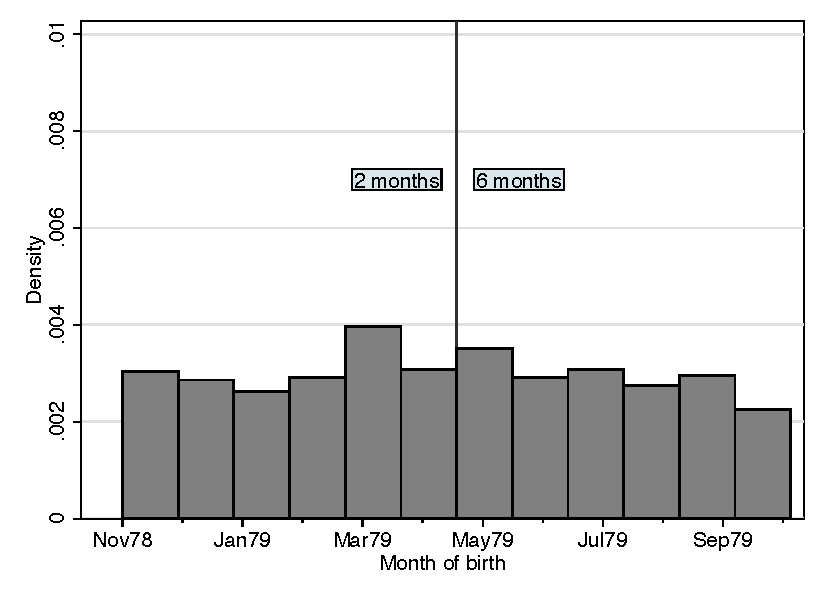
\includegraphics[width=0.8\textwidth]{../../analysis/graphs/SOEP/fertilityhist.pdf}
\caption{Fertility histogram for 1979 expansion in maternity leave legislation}\label{fig: fertilityhist_treated}
\begin{minipage}{\textwidth} % choose width suitably
{\footnotesize \textit{Note:} The histogram uses one month bins. The solid vertical line divides pre- and post-reform time span, i.e. two or six months of job-protected maternity leave after childbirth.\newline \textit{Source: }German Socio-Economic Panel, version 31\par}
\end{minipage}
\end{figure}






In the following, we present evidence for the balance of important predetermined parental variables of children born shortly before and after the threshold date. In the choice of dependent variables we follow the example of \cite{Dahl2016Case}, who focus on parental age at childbirth and average years of schooling. Moreover, we also consider parental nationality. \newline  Figures \ref{fig:yrschooling_parents_all cohorts}, \ref{fig:age_birth_all cohorts}  and \ref{fig:citizen_all cohorts} show average years of schooling, average age at childbirth and the percentage of German citizenship for mothers and fathers respectively for the four birth cohorts of the treatment and control groups (i.e. individuals born up to two years before and one year after the treated cohort). Over the four years there is some moderate fluctuation in predetermined characteristics, which can be attributed to the small sample size. However, most importantly, it seems that there are no conspicuous features around the cutoffs. Figures \ref{fig:yrschooling_parents_treated cohorts}, \ref{fig:age_birth_treatment cohort} and \ref{fig:citizen_treatment cohort} zoom into the preceding pictures and only consider the treated cohort. There is no polynomial structure that hints towards discontinuities in parental predetermined characteristics.  \newline Table \ref{tab:parental_covariate_balance} further supports the conclusions that were drawn from previous graphical impressions. The table presents for each cohort various means of pre- and postreform parental outcomes,  corresponding difference-in-means estimators (columns 3,6,9 and 12) and DD-RD estimates (column 13) as described by equation \ref{eq:RD+DD}. One can see that the the groups before and after the threshold are all very similar with respect to parental pre-determined characteristics, indicated by no single significant difference-in-means nor DD-RD estimator.\newline% There is no significant coefficient in neither one of the control cohorts nor in the treatment cohort, which would imply statistically significant differences with respect to parental pre-birth characteristics around the threshold dates. Additionally, neither one of the DD-RD estimates, which combine the four cohorts, indicate any changes in the distribution of parental observed characteristics as a response to the reform. %Without any significant estimate out of 30 in total is less than would be expected by pure chance and is thus no reason of concern. [DLMS: F-test for joint significance of parameters, but all my coefficients are zero anyways. So is it even necessary?]\newline


The preceding tables and figures support the choice of empirical strategies described in Section \ref{sec: estimation strategies}. Summing up, groups around the threshold are similar with no indication for sorting in the more generous maternity leave regime based on observed parental characteristics. For this reason, the occurrence of birth can be taken as a random event \citep{ekberg2013parental} and thus the expansion in maternity leave acts as a true natural experiment as described in \cite{rosenzweig2000natural}.\newline
Nonetheless, to scrutinize the possibility that the identification strategy is not jeopardized by selective fertility changes, we analyze the robustness of the results by applying a Donut specification. Furthermore, we examine whether the results change if pre-determined characteristics are included in the regressions (Section \ref{sec: robustness}). This can be motivated by the fact that pre- and post-threshold are very similar with respect to predetermined characteristics, but not entirely identical. By including pre-birth characteristics, one can see whether these differences matter for the results.




%\thispagestyle{empty}\fancyhf{}
%\chead{MATERNITY LEAVE AND LONG-RUN HEALTH OUTCOMES}
%\chead{Maternity leave and long-run child health}
%\rhead{\thepage}
%\renewcommand{\headrulewidth}{0.5pt}

%\newgeometry{
%	top    = 3.5cm,
%	bottom = 2cm,
%	left   = 5.0cm,
%	right  = 2.8cm}
%	
	
	
\begin{landscape}
\begin{table}[p]\centering
\begin{adjustwidth}{-2.5cm}{}

\def\sym#1{\ifmmode^{#1}\else\(^{#1}\)\fi}
\scalebox{0.9}{
\begin{tabular}{l*{16}{c}}
\toprule
Group &\multicolumn{3}{c}{Control 1 (Nov76-Oct77)} & & \multicolumn{3}{c}{Control 2 (Nov77-Oct78)} & & \multicolumn{3}{c}{Control 3 (Nov79-Oct80)}& &\multicolumn{4}{c}{Treatment (Nov78-Oct79)} \\ 

\cmidrule(lr{1em}){2-4} \cmidrule(lr{1em}){6-8} \cmidrule(lr{1em}){10-12} \cmidrule(lr{1em}){14-17}


            &\multicolumn{1}{c}{(1)}&\multicolumn{1}{c}{(2)}&\multicolumn{1}{c}{(3)}& &\multicolumn{1}{c}{(4)}&\multicolumn{1}{c}{(5)}&\multicolumn{1}{c}{(6)}& &\multicolumn{1}{c}{(7)}&\multicolumn{1}{c}{(8)} &\multicolumn{1}{c}{(9)}& &\multicolumn{1}{c}{(10)}&\multicolumn{1}{c}{(11)}&\multicolumn{1}{c}{(12)}&\multicolumn{1}{c}{(13)}\\
            &\multicolumn{1}{c}{$\mathbb{E}_{Pre}[Y]$}&\multicolumn{1}{c}{$\mathbb{E}_{Post}[Y]$}&\multicolumn{1}{c}{Raw $\Delta$} & &\multicolumn{1}{c}{$\mathbb{E}_{Pre}[Y]$}&\multicolumn{1}{c}{$\mathbb{E}_{Post}[Y]$}&\multicolumn{1}{c}{Raw $\Delta$} & &\multicolumn{1}{c}{$\mathbb{E}_{Pre}[Y]$}&\multicolumn{1}{c}{$\mathbb{E}_{Post}[Y]$}&\multicolumn{1}{c}{Raw $\Delta$} & &\multicolumn{1}{c}{$\mathbb{E}_{Pre}[Y]$}&\multicolumn{1}{c}{$\mathbb{E}_{Post}[Y]$}&\multicolumn{1}{c}{Raw $\Delta$}&\multicolumn{1}{c}{DD-RD}\\
\midrule 
\\
\textbf{Education }\\
\hline
%%%%%%%%%%%%%%%%%%%%%%%%%%%%%%%%%%%%%%%%%%%%%%%%%%%%%%%%%%%%%%%%%%%%
Mother & 11.070 & 10.715 & -0.355 &  & 10.788 & 10.800 & .012 &  & 11.026 & 11.140 & .114 &  & 11.531 & 11.271 & -0.260 & -0.196 \\ 
 &  &  & (0.464) &  &  &  & (0.382) &  &  &  & (0.358) &  &  &  & (0.465) & (0.515) \\ 

Father & 11.532 & 11.609 & 0.077 &  & 11.802 & 11.687 & -0.115 &  & 11.395 & 11.828 & 0.433 &  & 12.464 & 11.811 & -0.652 & -0.809 \\ 
 &  &  & (0.621) &  &  &  & (0.511) &  &  &  & (0.416) &  &  &  & (0.569) & (0.633) \\ 






%%%%%%%%%%%%%%%%%%%%%%%%%%%%%%%%%%%%%%%%%%%%%%%%%%%%%%%%%%%%%%%%%%%% 
 \\
\textbf{Age at childbirth }\\
\hline
Mother & 26.264 & 26.153 & -0.112 &  & 27.575 & 26.484 & -1.091 &  & 26.659 & 26.984 & 0.326 &  & 26.919 & 27.586 & 0.667 & 0.893 \\ 
 &  &  & (0.749) &  &  &  & (0.666) &  &  &  & (0.653) &  &  &  & (0.693) & (0.790) \\ 
Father & 29.896 & 29.099 & -0.796 &  & 30.366 & 29.833 & -0.532 &  & 29.488 & 29.942 & 0.454 &  & 30.673 & 30.802 & 0.129 & 0.360 \\ 
 &  &  & (0.759) &  &  &  & (0.737) &  &  &  & (0.770) &  &  &  & (0.738) & (0.854) \\ 


%%%%%%%%%%%%%%%%%%%%%%%%%%%%%%%%%%%%%%%%%%%%%%%%%%%%%%%%%%%%%%%%%%%%
\\
\textbf{Nationality}\\
\hline 
Mother & 0.905 & 0.852 & -0.053 &  & 0.816 & 0.856 & 0.040 &  & 0.840 & 0.844 & 0.004 &  & 0.895 & 0.842 & -0.054 & -0.050 \\ 
 &  &  & (0.044) &  &  &  & (0.049) &  &  &  & (0.046) &  &  &  & (0.040) & (0.048) \\ 
Father & 0.823 & 0.821 & -0.002 &  & 0.839 & 0.832 & -0.007 &  & 0.832 & 0.858 & 0.026 &  & 0.863 & 0.824 & -0.039 & -0.040 \\ 
  &  &  & (0.054) &  &  &  & (0.050) &  &  &  & (0.045) &  &  &  & (0.047) & (0.053) \\ 

\bottomrule
\end{tabular}
}
\caption{Parental pre-determined characteristics, treatment and control cohorts}\label{tab:parental_covariate_balance}
\begin{minipage}{1.75\textwidth} % choose width suitably
{\footnotesize \textit{Note:} This table reports descriptive statistics of pre-birth parental characteristics for different cohorts of fathers and mothers, who became parents between November 1976 and October 1980. The first two columns list per cohort average outcomes of parents within half a year before or after the cutoff day respectively. Columns (3), (6), (9) and (12) show difference-in-means estimators for these parental outcomes. Column (13) reports DD-RD estimates according to equation \ref{eq:RD+DD}. 
Clustered standard errors are reported in parentheses. Significance levels: + \(p<0.15\), * \(p<0.10\), ** \(p<0.05\), *** \(p<0.01\). \newline \textit{Source: }German Socio-Economic Panel, version 31\par}
\end{minipage}
\end{adjustwidth}
\end{table}

\end{landscape}






\subsection{Long-run child health outcomes in response to the expansion in maternity leave}\label{sec: health outcomes}
The goal of the two identification designs described in Section \ref{sec: estimation strategies} is to estimate intention-to-treat effects for individuals whose mothers differ in their eligibility for prolonged maternity leave, but the children and their mothers are otherwise equivalent. \newline


Before estimating the intention-to-treat estimates of the impact of the expansion in maternity leave on child health outcomes, a natural starting point is to investigate maternal labor market outcomes as a response to the expansion in maternity leave. If, for example, women return to work later, there is a chance that the reform changed something in the care for the newborn and hence child development as described in Section \ref{sec: 2.1 mechanism}. However, as already mentioned, there is no information on maternal labor market outcomes after childbirth.\footnote{This is due to the fact that the SOEP was initiated after the legislation change occurred.} Nevertheless, \cite{dustmann2012expansions} have explored this matter with administrative data from the IAB (Institute for Employment Research Nuremberg). They find that mothers stay on average 0.8 months longer away from work and have more cumulative income if they fall under the new, more generous leave scheme.\newline

In this section, we present the intention-to-treat estimates of the impact of an expansion in maternity leave on children's long-term health outcomes, which are observed over the period 1993-2014. We use both a (i) RD and (ii) DD-RD design. The focus is in each case on biometric, objective, subjective health and health behavior outcomes. Subsequent sections consider ITT effects for each year of children's adult life, for different subgroups and potential mechanisms that may be responsible for the effects.

\bigskip
\underline{\textbf{(i) RD design}}\\
In the first step, we carry out a pure regression discontinuity analysis (see equation \ref{eq:RD}) for different orders of $f(\cdot)$. The outcomes are observed over the period 1993-2014. The RD evaluation is performed in order to get a first idea of the impacts of maternity leave on long-run child health, which can serve as benchmark for the following analysis. Because there is only few data around $c$, one might choose a more complex $f(\cdot)$ in order to capture the variation of the data.\newline 
Figures \ref{fig: RD_BM} - \ref{fig: RD_HB} and Tables 
\ref{tab:RD_BM} - \ref{tab:RD_HB} report results in graphical and numerical format. We estimate the equation for linear, quadratic and cubic functions of $\tilde X_{im}$ and a linear Donut specification in which individuals born within one month from the cutoff date are excluded from the analysis.
The tables provide mixed evidence whether the expansion in maternity leave is beneficial or harmful for adulthood health. Oftentimes, coefficients are not significant or contradictory. \newline
There is unanimous evidence that children born under the new regime are shorter in adulthood, but less likely to be overweight/obese. Especially for objective health outcomes there are often no congruent estimates, i.e. there are different signs of coefficients for different orders of $f(\cdot)$ for the same outcome. Yet, for subjective health measures there is a more consistent picture.\footnote{The successive sections show that the point estimates for subjective health outcomes are always among the most significant ones.} Respondents whose mothers were entitled to longer maternity leave are more concerned about their health, have lower perceptions about their current health status, are less satisfied about their sleep and their state of health limits their activities more often. For the remaining subjective health variables the effect is not clear. For the health behavior there is conclusive evidence that children consume more alcoholic beverages in adulthood in response to the reform. \newline
From the preceding discussion, one can see that it is quite difficult to make a solid statement whether the reform was harmful or beneficial for adulthood health over the period 1993-2014. This is closely connected to the problem of a relatively small sample size within the bandwith of the cutoff date.
Overall, the presented figures and tables provide no support for the hypothesis that the expansion in maternity leave had a positive impact on children's long-run health outcomes. If there is any effect, it seems that the expansion in maternity leave has a detrimental effect on long-run health outcomes. For that reason it seems advisable to work with another identification approach (DD-RD design, which can can make use of more observations and does not depend on the right functional form of $f(\cdot)$.)

\bigskip
\underline{\textbf{(ii) DD-RD design}}\\
In this subsection, DD-RD estimates are presented that are based on equation \ref{eq:RD+DD} in Section \ref{sec: estimation strategies}. Table \ref{tab:Healthoutcomes_DDRD} summarizes the ITT effects for different sets of health outcomes. The sample includes children that were born within 6 months of the threshold date, but not only for the treatment cohort but also two years before and one year after the treatment year as control cohort. The outcomes are observed over the period 1993-2014. \newline
Table \ref{tab:Healthoutcomes_DDRD} confirms the impression from the preceding section. If there are long-run health effects, they are negative. 
Children born under the new regime are on average 0.16 cm larger, weigh 1 kg more, have a 0.31 points larger BMI and are 3\% percent more likely to be overweight or obese over the period 1993-2014.\footnote{All following estimates in this section are associated with ITT effects over the period 1993-2014, even when it is not explicitly mentioned.} However, none of these effects is statistically different from zero. 
Concerning objective health outcomes, some of the estimates are significant, contrary to the RD design. Respondents under the new maternity leave regime are on average more likely to be sick and consult a doctor. However, the effects are only significant at the intensive margin, with 2.3 more days sick and 0.432 times more doctor consultations. The point estimates are also positive, but not significant, for the likelihood of hospital stays, to be legally handicapped and to suffer from a disease as defined in Section \ref{sec:variables}. The point estimate for suffering from a chronic disease is positive and statistically significant from zero on a significance level of 15\%.
As it has been already the case with RD results, the strongest and most significant results can be found in the domain of subjective health outcomes. Children born under the new regime are more concerned about their health, assess themselves a lower health status, their state of health limits their activities more often and they are more socially limited. Furthermore, they are less satisfied with their sleep (borderline significant at a 15\% level), handle stress worse and have strong physical pain more often in the last four weeks (not significantly different from zero).
Concerning the health behavior, the point estimates indicate that the children under the new reform are on average more likely to smoke (both at the extensive and intensive margin) and sleep less, both during weekdays and weekend. They are also less likely to follow a health-conscious diet and have a private health insurance, and more likely to consume alcoholic beverages, whereas these effects are not significantly different from zero.\newline



In order to determine whether the health effects in response to the expansion in maternity leave are of a medium- or long-term nature, the next section presents an analysis in which the entire period from 1993 to 2014 is disaggregated into each interview year separately. 






%\thispagestyle{empty}\fancyhf{}
%%\chead{MATERNITY LEAVE AND LONG-RUN HEALTH OUTCOMES}
%%\chead{Maternity leave and long-run health outcomes}
%%\rhead{\thepage}
%\renewcommand{\headrulewidth}{0pt}



	
	
\begin{landscape}

\begin{table}[htp] \begin{adjustwidth}{-2cm}{}

 \centering  \vspace{-1cm} 
\def\sym#1{\ifmmode^{#1}\else\(^{#1}\)\fi}
\vspace*{\fill}
\caption{Health outcomes, Difference-in-difference Regression Discontinuity}\label{tab:Healthoutcomes_DDRD}

\begin{tabular}{l*{10}{c}}
\toprule
 &\multicolumn{1}{c}{(1)}&\multicolumn{1}{c}{(2)}&\multicolumn{1}{c}{(3)}&\multicolumn{1}{c}{(4)}&\multicolumn{1}{c}{(5)}&\multicolumn{1}{c}{(6)}&\multicolumn{1}{c}{(7)}&\multicolumn{1}{c}{(8)}\\ 
\midrule\\

\textbf{Biometric Outcomes}\\

	          &\multicolumn{1}{c}{Height}&\multicolumn{1}{c}{Weight}&\multicolumn{1}{c}{BMI}&\multicolumn{1}{c}{D\_overw\_obese}\\
\midrule
      &    0.159         &    1.192         &    0.306         &   0.0391         \\
          &  (1.261)         &  (2.354)         &  (0.636)         & (0.0581)         \\

	\midrule
	\(N\)     &     4560         &     4506         &     4503         &     4503         \\

	\\ \\
	\textbf{Objective Health}\\
        
        
               &\multicolumn{1}{c}{D\_sick}&\multicolumn{1}{c}{Days\_sick}&\multicolumn{1}{c}{D\_doctor}&\multicolumn{1}{c}{Docvisits}&\multicolumn{1}{c}{D\_hospital}&\multicolumn{1}{c}{D\_disab}&\multicolumn{1}{c}{D\_illness}&\multicolumn{1}{c}{D\_chronill}\\
\midrule
       &   0.0506         &    2.259\sym{*}  &   0.0437         &    0.432\sym{*}  &   0.0213         &  0.00941         &   0.0771         &   0.0655\sym{+}  \\
          & (0.0366)         &  (1.271)         & (0.0308)         &  (0.236)         & (0.0164)         & (0.0139)         & (0.0687)         & (0.0442)         \\

     \midrule
     \(N\)     &     9709         &     9709         &    13523         &    13564         &    13658         &    13810         &     1566         &     4841         \\

	\\ \\
	\textbf{Subjective Health}\\
	         
        
               &\multicolumn{1}{c}{Health\_concerns}&\multicolumn{1}{c}{SAH\_5}&\multicolumn{1}{c}{SAS\_10}&\multicolumn{1}{c}{Problems\_activ}&\multicolumn{1}{c}{Handle\_stress}&\multicolumn{1}{c}{Phys\_pain}&\multicolumn{1}{c}{Constr\_soc}\\
\midrule
       &    0.162\sym{***}&   -0.208\sym{***}&   -0.339\sym{+}  &   0.0895\sym{*}  &   -0.178         &    0.111         &    0.140\sym{*}  \\
          & (0.0547)         & (0.0662)         &  (0.211)         & (0.0467)         &  (0.205)         & (0.0885)         & (0.0780)         \\

     \midrule
     \(N\)     &    10611         &    13821         &     6474         &     4574         &     1658         &     4562         &     4560         \\

	\\ \\
	\textbf{Health Behavior}\\
        
               &\multicolumn{1}{c}{Healthydiet}&\multicolumn{1}{c}{D\_smoke}&\multicolumn{1}{c}{Cigarettes}&\multicolumn{1}{c}{Alcohol}&\multicolumn{1}{c}{D\_privHI}&\multicolumn{1}{c}{hrsleep\_wrk}&\multicolumn{1}{c}{hrsleep\_wknd}\\
\midrule
      &   -0.108         &   0.0950\sym{*}  &    2.209\sym{*}  &  -0.0574         & -0.00584         &   -0.242\sym{**} &   -0.326\sym{**} \\
          & (0.0849)         & (0.0561)         &  (1.195)         &  (0.137)         & (0.0279)         &  (0.100)         &  (0.127)         \\

     \midrule
     \(N\)     &     3675         &     3997         &     1949         &     1703         &    13784         &     5579         &     5565         \\

     \bottomrule
\end{tabular}
\vspace*{\fill}

\begin{minipage}{1.7\textwidth} % choose width suitably
{\footnotesize \textit{Note:} This table reports various DD-RD estimates of the impact of the expansion of maternity leave from two to six months on different sets of health outcomes. The estimates are based on equation \ref{eq:RD+DD}. The control group is comprised of children that are born in the same months but two years before and one year after the reform (i.e. children born between November 1976 and October 1977, November 1977 and October 1978, and November 1979 and October 1980). The outcomes are measured over the period 1993-2014.  \newline
Clustered standard errors are reported in parentheses. Significance levels: + \(p<0.15\), * \(p<0.10\), ** \(p<0.05\), *** \(p<0.01\). \newline \textit{Source: }German Socio-Economic Panel, version 31\par}
\end{minipage}
 \end{adjustwidth}

\end{table}

\end{landscape}









\bigskip
\subsection{Life-course approach}\label{sec: lifecourse approach}

In the following, we estimate the impact of the 1978 expansion in maternity leave from two to six months on health outcomes over the life-course. While the previous estimates in Section \ref{sec: health outcomes} provide intention-to-treat effects over the entire period 1993-2014, the following life-course approach explores whether these effects are more of a medium- or long-term nature. In order to do so , we compute ITT effects for each outcome associated with each interview year, i.e. run regressions based on equation \ref{eq:RD+DD} for each year.\footnote{For the variable \texttt{Handle\_stress} we cannot conduct the life-course approach due to the fact that there are just too few observations per each interview year.} In this way we capture a time window in which the respondents are between 17 and 37 years old. The results can be found in Figures \ref{fig: LC_BM} - \ref{fig: LC_HB}, which depict DD-RD estimates along with 90\% Confidence intervals by each year of respondent's adulthood life. Note that for some variables, we had to adjust the life-course approach and compute the ITT effect for every other year due to the frequency of the variable in the household survey. For the same reason the life-course for different variables are not necessarily of equal length.

Overall, the figures suggest that the intention-to-treat effects of the expansion in maternity leave on health outcomes do not seem to be especially driven by either medium- or long-term effects. For each figure, particularly the ones for which there are no significant point estimates in Table \ref{tab:Healthoutcomes_DDRD}, the majority of the ITT effects are not significantly different from zero. If there are spikes, then they occur over all values of the life-course, but they are never significantly different from zero for many years in a row. For these reasons, it does not seem that the health outcomes under consideration are persistently affected by the maternity leave reform over the study-period 1993-2014. 





\bigskip
\subsection{Heterogeneous intention-to-treat effects}\label{sec: heterogeneous TE}

%Hier bereits die Einleitung anpassen: andere Art von heterogeneity analysis, LC war ja bereits auch eine Art Heterogeneity analysis 

While the previous sections explore overall ITT estimates for the entire period from 1993 - 2014 and for each interview year separately, this section presents heterogeneous impacts of the legislation change in maternity leave on health outcomes, including separate estimates for different subgroups. The heterogeneity analysis is being carried out in order to identify subgroups that react differently to the reform both in terms of sign and magnitude. These insights can help to redesign parental leave policies in order to better fit target populations.\newline First, the intention-to-treat effects are distinguished by gender, whether respondents have an (indirect) migration background, whether they are married or have children, whether their annual inflation-adjusted household labor income is below the median as well as by the educational attainment of themselves and their parents.\footnote{Parental educational attainment refers to the highest one achieved by either the mother or the father.} Tables \ref{tab:Heterog_BM} - \ref{tab:Heterog_HB} present the DD-RD estimates for the different subgroups. The first row shows the effects for the entire sample population, which are the same as in Table \ref{tab:Healthoutcomes_DDRD}. \newline
Second, we present a spatial differentiation of the reform's impact on adulthood health outcomes by federal state.

All other factors are the same as in Section \ref{sec: health outcomes} (ii).\footnote{This also implies that the point estimates correspond to impacts of the change in maternity leave legislation on adulthood health outcomes over the period 1993-2014. } In the following, we discuss some results for each set of health outcomes before the spatial impacts of the reform are presented.\footnote{In light of the high quantity of significant estimates, this section provides a selection of some of the most interesting cases. More information can be found in Tables \ref{tab:Heterog_BM} - \ref{tab:Heterog_HB}.} \newline

\begin{enumerate}[(i)]
\item \underline{Biometric Health Outcomes} \\ Although there are no significant effects on total ITT for biometric health outcomes, one can find significant effects for various subgroups in Table \ref{tab:Heterog_BM}. For instance, the height point estimate for women is negative, indicating that women born under the more generous leave scheme are comparatively shorter over the period 1993-2014. Having a migration background does not matter for the impact of the reform on biometric health outcomes. The reform causes on average a higher incidence rate of being overweight or obese for unmarried respondents and individuals who graduated from the middle track.
% Respondents, which are not married suffer more from the reform, because they are on average significantly more likely to be overweight and/or obese. Respondents with children benefit more from the reform, due to the fact that they are on average 2.8 cm larger. The expansion in maternity leave is detrimental for respondents that completed the middle track, as they are on average heavier, possess over a higher BMI and are more likely to be overweight. Respondents with a degree from the highest track however benefit in terms of a higher body height. Same holds for respondents whose parents completed the middle track.

\item \underline{Objective Health Outcomes}\\Table \ref{tab:Heterog_OH} shows that men react to the expansion in leave coverage much more than women. They are on average sick more often and visit a doctor more frequently (both at the extensive and intensive margin). Women, however, are more likely to be diagnosed with a longstanding illness as defined in Section \ref{sec:variables} in response to the reform. Respondents below the median household labor income, which were born shortly after the expansion in maternity leave legislation, visit a doctor more often, both at the extensive and intensive margin. %People with a degree from the lowest track are more sick and go to the doctor more often. Respondents with a degree from the second track are more often sick,  hospitalized and diagnosed with a longstanding disease. And individuals who graduated from the highest track have more doctor consultations and are more often chronically ill. The effects of the reform on individuals whose parents have a degree from the lowest track are significant with respect to being sick and doctor visits.

\item \underline{Subjective Health Outcomes}\\ Table \ref{tab:Heterog_SH} presents the heterogeneous results for the subjective health outcomes. Being in line with previous results, the most significant estimates are among subjective health outcomes, suggesting that the expansion in maternity leave had the strongest effect on this type of health outcomes over the period from 1993 to 2014.\newline
The impact of the reform on concerns about own health is equally present regardless of gender, migration background, marital status and having children. The impact of the expansion in maternity leave on self-assessed health is greater for women, unmarried individuals, respondents without children, individuals with a household labor income below the median, because they judge their current health on average worse for the period from 1993 until 2014. The reform had only a small impact on how respondents can handle stress, and it only affects respondents with a household income below the median and a degree from the lowest track significantly (different signs).

\item \underline{Health Behavior}\\
The heterogeneous impacts of the 1978 expansion in maternity leave on long-run health behavior are presented in Table \ref{tab:Heterog_HB}. Even though the overall impact on following a health-conscious diet was insignificant, married, respondents with children and with a degree form the middle track are less likely to follow a health-conscious diet if they were born shortly after the legislation change. The effect of the reform on the amount of sleep during weekdays is significant for women, married, respondents below the median for household labor income and respondents with a degree from the highest track, because they sleep less on average over the period from 1993-2014. 
\end{enumerate}


% DISCUSSION BY FEDERAL STATE:
\newpage
\underline{\textbf{Impact maps}}\newline
In the following, we estimate the \emph{spatial} impact of the expansion in maternity leave coverage on children's long-run health outcomes in order to see whether the effects described in Section \ref{sec: health outcomes} (ii) are different across federal sates. If there is great spatial heterogeneity across federal states, then this could help to find determinants for the impact's sign. Figures \ref{fig: LOC_BM} - \ref{fig: LOC_HB} show intention-to-treat estimates for each variable by federal states.\footnote{Please note that the figures do not show the "new" federal states Brandenburg, Mecklenburg-Vorpommern, Saxony, Saxony-Anhalt and Thuringia as they were part of the former GDR.} The figures are created by estimating and plotting ITT effects based on equation \ref{eq:RD+DD} for each federal state using an ESRI shapefile. \newline
In general, the figures indicate that the federal states whose economies have been performing traditionally better are on average more often subject to beneficial impacts and vice versa. This implies that the economic circumstances and also the average economic prosperity (i.e. the average (parental) SES of a federal state's population) are important determinants for the success of maternity leave. This point is further discussed in Section \ref{sec: Conclusion}.\newline \bigskip


Section \ref{sec: 2.1 mechanism} describes positive impacts of the expansion in maternity leave on children's health in the long-run, conditional on having improved maternal care due to the reform. After having investigated ITT effects over the entire period from 1993-2014, for each year separately and for different subgroups, it seems that there is little evidence that the expansion in maternity leave has improved children's health in the long-run. The results suggest quite the opposite, as many health variables are negatively influenced for those, who were born shortly after the legislation change. The estimates indicate that in particular for many subjective - and some objective health variables.\newline
Overall, the heterogeneity analysis shows that intention-to-treat effects of the reform are worse for men, respondents with no children, for people with an annual household income below the median and individuals whose parents have a school certificate from the lowest track. The spatial investigation adds to the conjecture that socio-economic status (either by the parents or the general level of the federal state) is decisive for successful parental leave mandates, as the effects are more often positive in economically strong federal states. This raises the question whether maternity leave mandates should be redesigned, because privileged parents could use the expansion in paid leave better. The original goals of parental leave mandates were noble, but the results suggest that the reform led to a deterioration of health inequality. In that respect, maternity leave can be seen as a potential intergenerational transmission mechanism for health.






%\begin{itemize}
%\item badly designed policy - children with parents of low SES are particularly harmed by the reform %LINDEBOOM REFERENCE
%\item For more privileged individuals we also see worse self-assessed health, why is that the case?
%\begin{itemize}
%\item Better self-awareness 
%\item or is this due to reporting error, better educated report their health more accurately [reference: \cite{cawley2015health}]
%\end{itemize}
%\item ITT effects depend on quality of caregiver $\rightarrow$ children form low SES parents would have benefited more from alternative caregiver than from parents?
%\item intergenerational transmission mechanism for health strengthened - health inequality further manifested
% 
%\end{itemize}



 The next section considers potential mechanisms that may explain how the legislation change in maternity leave can affect health outcomes in adulthood.


\newpage
\subsection{Potential mechanisms}\label{sec: channels}
The preceding analysis shows that there are significant effects of the legislation change in maternity leave on health outcomes. The objective of this section is to investigate how the reform could affect health outcomes. While Section \ref{sec: 2.1 mechanism} introduced various mechanisms from the parents' perspective, this section explores pathways from the child's point of view. Following the literature, educational attainment, family and labor market outcomes are considered as potential mechanisms. \newline 

The relationship between socioeconomic status (SES) and health outcomes is a well established finding in the social sciences. People with better financial background, education and labor market outcomes tend to be healthier on average \citep{currie2003socioeconomic}. This finding is persistent across age, gender and appears at all parts of the SES distribution \citep{Donell}. In the literature there is still a debate whether the SES health gradient (disparities in health across socioeconomic status) is driven by the impact of SES on health or vice versa. In the analysis we focus on the impact of SES on health in order to obtain possible mechanisms how the expansion in maternity leave can affect health outcomes. \newline 
Since the early 2000s the research on long-run effects of early childhood development has took off quite rapidly. Shocks in early life can have persistent effects on adulthood economic, social and health outcomes \citep{heckman2013understanding}. The focus in economics lies often on cognitive skill formation, educational attainment and labor market outcomes. \cite{currie2011human} advocate to not underestimate influences that originated decades ago. They emphasize that child and family characteristics measured at school entry do as much to explain future outcomes as factors that (labor) economists have more traditionally focused on, such as years of education.\newline

In the following, you can find an ad-hoc motivation why educational attainment, family outcomes (marriage and fertility characteristics) and labor market outcomes are considered as potential pathways whereby the legislation change in maternity leave can affect long-run health.\newline
There is both theoretical and empirical evidence that education can influence health outcomes. More years of education are associated with better self-assessed health, lower mortality rates and higher levels of population health.\footnote{ See \cite{arendt2005does}, \cite{lleras2005relationship} and
\cite{cutler2006education}.} In the domain of labor market outcomes, there is evidence that higher income levels are connected to better health, while unemployment is thought to harm health and evoke adverse health behavior.\footnote{See \cite{galama2015theory}, \cite{currie2009healthy}, \cite{sullivan2009job}, \cite{salm2009does} and \cite{garrouste2015lasting}.} Marital status is found to reduce the incidence of mental illness and mortality.\footnote{See \cite{gove1983does} and \cite{roelfs2011rising} .} The effect of having children may be both detrimental and beneficial for somebody's health and depends largely on the marital status. Unmarried parents are relatively more affected by depression and lower self-esteem, while married individuals suffer less from depression but are exposed to more marital conflict compared to their childless counterparts \citep{nomaguchi2003costs}.\newline

In order to explore these mechanisms we estimate intention-to-treat effects of the expansion in maternity leave on education, family and labor market outcomes according to equation \ref{eq:RD+DD} in Section \ref{sec: estimation strategies}.\footnote{Similar to Section \ref{sec: health outcomes}, we consider outcomes over the entire period 1993-2014.} Table \ref{tab: mechanisms} presents various DD-RD estimates of the reform's impact on the channeling outcomes. It is found that the reform caused individuals to frequent the lowest school track more often at the expense of the other two. Moreover, the average years of schooling increased in response to the reform. Yet, none of the effects is significantly different from zero. Family outcomes are borderline significant (on a 15\% level) and show that respondents are on average more likely to be married and have children. Finally, children born shortly after the reform are on average less likely to be employed and have a lower household labor income over the period 1993-2014.\newline

The results on educational choices and labor market outcomes obtained in Table \ref{tab: mechanisms} are verified by \cite{dustmann2012expansions}. They find inconclusive and insignificant difference-in-difference estimates for children's track choice and positive yet insignificant estimates for the average years of schooling. Their point estimates for wages are throughout negative, and they get conflicting evidence for full-time employment; again both insignificant. So the sign of our estimates are always congruent with most of theirs. Their results contrast with ours only by the significance for labor market outcomes. One difference between their approach and ours is that they only consider outcomes at age 28, whereas we have outcomes over the entire period 1993-2014. This enables us to better capture different stages of life, e.g. at labor market entry and at later career stages.\newline 

The main takeaway from this analysis is that we can exclude educational outcomes as potential mechanisms how the reform could affect respondents' health. This finding is in line with the results of \cite{dustmann2012expansions}. Labor market outcomes suggest to be significantly negatively affected by the reform (in particular the likelihood of being unemployed), which could be one explanation for the health differential between the individuals born around the threshold date. Due to the ambiguity of the family outcomes (at least for having children), they can be also a channel how the legislation change affected health outcomes. Of course this is merely suggestive evidence for the potential channels that allow the reform to affect health outcomes.\newline

A promising extension to this analysis would be to investigate (short-run) parental health outcomes in response to the reform.\footnote{This analysis is not being carried out here, due to the fact that the SOEP only started in 1984, which would be too late to capture short-term health differentials.} If there were changes in parental health outcomes (induced by the expansionary policy reform) such as more stress, depression or poor health in general, then this could explain effects on long-run health outcomes of the children.\footnote{Worse health is expected to hamper parental ability to nurture, which may be an explanation for the children's health differentials in adulthood.} \newline Another auspicious possibility for future research is to construct a structural model, in which one models long-run effects and mechanisms of labor market, family and health outcomes \citep{garrouste2015lasting}.


\begin{table}[p] \centering
\def\sym#1{\ifmmode^{#1}\else\(^{#1}\)\fi}
\begin{tabular}{l*{10}{c}}
\toprule
	& \multicolumn{1}{c}{(1)} & \multicolumn{1}{c}{(2)} & \multicolumn{1}{c}{(3)} & \multicolumn{1}{c}{(4)} \\
	\midrule
	\\
\textbf{Educational attainment}\\
\midrule
            &\multicolumn{1}{c}{Track 1}&\multicolumn{1}{c}{Track 2}&\multicolumn{1}{c}{Track 3}&\multicolumn{1}{c}{Yrs\_schooling}\\
\midrule
        &      0.0282         &     -0.0659         &    -0.00242         &       0.122  \\       
            &    (0.0474)         &    (0.0499)         &    (0.0542)         &     (0.279)         \\
\\

\textbf{Family outcomes}\\
\midrule
&\multicolumn{1}{c}{D\_married}&\multicolumn{1}{c}{D\_child}\\
\midrule
&      0.0631\sym{+}  &      0.0711\sym{+}  \\
&    (0.0425)         &    (0.0474)        \\
\\
\textbf{Labor market outcomes}\\
\midrule
&\multicolumn{1}{c}{D\_employed}&\multicolumn{1}{c}{HHInc}\\
\midrule
&     -0.0547\sym{**} &     -4669.1\sym{+}  \\
 &    (0.0278)         &    (2862.6)         \\
\bottomrule


\end{tabular}
\caption{The impact of the expansion in maternity leave on child SES outcomes}\label{tab: mechanisms}
\begin{minipage}{\textwidth} % choose width suitably
{\footnotesize \textit{Note:} This table reports various DD-RD estimates of the impact of the expansion in maternity leave from two to six months on different sets of educational, family and labor market outcomes over the period 1993-2014. The estimates are based on equation \ref{eq:RD+DD}. The control group is comprised of children that are born in the same months but two years before and one year after the reform (i.e. children born between November 1976 and October 1977, November 1977 and October 1978, and November 1979 and October 1980). \newline
Clustered standard errors are reported in parentheses. Significance levels: + \(p<0.15\), * \(p<0.10\), ** \(p<0.05\), *** \(p<0.01\). \newline \textit{Source: }German Socio-Economic Panel, version 31\par}
\end{minipage}
\end{table}





%[other Channel possibility: assortative matching? Partners with less education....]


% NOTES TO BE INCLUDED: SOME VARIABLES MAY NOT BE BAD AS THEY SUGGEST; FOR EXAMPLE: MORE DOCTOR VISITS MAY BE EQUIVALENT WITH BETTER HEALTH KNOWLEDGE/AWARENESS, PRECAUTIONARY MOTIVES, preventative 






\newpage
%-----------------------------------------------------------------------------------------------------------------------------------
%	Robustness Check
%-----------------------------------------------------------------------------------------------------------------------------------
\subsection{Robustness}\label{sec: robustness}

  
Different measures to test the robustness of the results are carried out in this section. First, a covariate vector $Z_{imt}$ is included in the main specification (equation \ref{eq:RD+DD}). Second, we explore whether the results are any different, when the bandwidths are smaller or children that are born in the month before and after the threshold are deleted from the analysis. Third, the importance of the choice of control group is investigated by different placebo treatments and other compositions of control groups.\newline



\textbf{(i)Inclusion of covariates:} First, we repeat the heterogeneity analysis presented in Section \ref{sec: heterogeneous TE}, but with the difference that a covariate vector is added to the main DD-RD specification.\footnote{The covariate vector includes sex, migration background, age, squared age, parental type of school, parental citizenship and age at childbirth. The parental information is included for mothers and fathers individually.
%marital status, children and siblings dummies, school type, years of schooling, household labor income
} This gives the possibility to control for compositional changes of the treatment and control group, which might lead to non-parallel dynamics in outcome variables otherwise \citep{abadie2005semiparametric}. Furthermore, the additional explanatory variables describe the effect of the legislation change for different subgroups, such that one allows for heterogeneous ITT effects. This approach makes intuitively sense, because parental and individual background characteristics on both sides of the threshold are very similar to each other, yet not entirely identical. The difference-in-difference approach enables to easily add the characteristics to the regression equation.\newline
Tables \ref{tab:Heterog_BMCV} - \ref{tab:Heterog_HBCV} present the results and have the same structure as the ones from Section \ref{sec: heterogeneous TE}. The magnitude and significance of the estimates are robust to including the extra control variables, indicating that compositional changes of treatment and control group do not matter a lot.
% aus paper mit RD: sollte nix ausmachen wenn man covariates reinnimmt, da links und rechts individuen gleich sind abgesehne vom treatment.... 



\bigskip
\textbf{(ii) Different bandwidths and Donut specification:} Second, we test the sensitivity of the results using different bandwidths $h$ (use 3 – 6 months). Furthermore, a Donut specification is applied, in which children born in the month before and after the threshold (April \& May) are eliminated from the analysis. The Donut specification verifies that the results obtained in Sections \ref{sec: health outcomes}-\ref{sec: heterogeneous TE} are not biased by endogenous timing of birth. We only exclude one month on each side under the assumption that if there are any manipulations in the birth variable they will most likely occur around the threshold date (see Section \ref{sec:threats indentification} and \ref{sec: validity}). Tables \ref{tab:BMBW} - \ref{tab:HBBW} present overall impacts of the reform on health outcomes over the period 1993-2014 with different bandwidth choice and a Donut specification. The bandwidth is increased from three months in the most stringent specification to six months in the widest specification. The Donut specification also uses a bandwidth of six months, but excludes children born in April and May. The tables show that it is very unlikely that there is a bias due to endogenous timing of birth, because the estimates from the baseline specification with six months bandwidth and the Donut specification are highly similar to each other in terms of magnitude and significance. Concerning the bandwidth choice, some of the health effects disappear if the window around the threshold is chosen too narrowly.\footnote{This does not hold for most of the subjective health outcomes. They remain significant, even with very small bandwidths.} This is very likely related to the small sample size. When decreasing the bandwidth too much, there are too few observations on each side of the threshold. Consequently it is impossible to precisely estimate ITT effects any longer when making the bandwidth too narrow.

\newpage
\textbf{(iii) Dependence on the choice of control groups:} Finally, we test whether the results depend on the particular choice of control groups. On the one hand, additional years\footnote{The extra years are additional to the already existing ones of up to two years before and one year after the reform.}, in which no reform occurred are added to the sample in order to have more control cohorts. The results remain qualitatively the same when combining these cohorts in different compositions. On the other hand, we define placebo treatments, in which the treatment status is assigned to children, which were born in years, in which no legislation change took place. The resulting point estimates do not suggest significant impacts for these placebo treatments.\footnote{For example when keeping the threshold at May, but assigning the treatment status to control cohorts one (Nov76-Oct77), two (Nov77-Oct78) and three (Nov79-Oct80), we only obtain 3, 1 and 7 significant estimates in comparison to 11 overall significant results as depicted in Table \ref{tab:Healthoutcomes_DDRD}.}\newline

Overall, the different robustness checks provide evidence that the effects on health outcomes are driven by the legislation change in maternity leave from two to six months in 1979 and not by compositional changes in treatment and control group, the particular choice of bandwidth or the control group.



\bigskip%-----------------------------------------------------------------------------------------------------------------------------------
%	Summary & Discussion
%-----------------------------------------------------------------------------------------------------------------------------------
\section{Summary \& Discussion}
\label{sec: Conclusion}


In this article, we analyze the impact of a reform in maternity leave on children's long-run health outcomes. In order to estimate causal effects of maternity leave, we use exogenous variation in return to work decisions from a legislative change in the Federal Republic of Germany in 1979, in which the length of paid maternity leave was increased from eight weeks to six months after childbirth. We use a broad variety of health outcomes from the German Socio-Economic Panel, which are observed over the period 1993-2014. We find that the reform led to a decline in children's long-term health outcomes. Children born under the more generous regime are consulting doctors more often, have more sick days and are more likely to suffer from a chronic disease over the period 1993-2014. Additional evidence suggests that they have a worse perception and more concerns about their health, as well as more problems to carry out daily activities and they are more often socially constrained due to their health status. The intention-to-treat estimates further suggest that more maternity leave led children to indulge in more unhealthy behavior such as smoking and less hours of sleep. A life-course approach reveals that the effects are not only driven by either medium- or long-term effects. A heterogeneity analysis shows that men, respondents without children, persons with an annual household labor income below the median and whose parents have a school certificate from the lowest track, are particularly harmed by the expansionary reform. Furthermore, there is differential reporting behavior with respect to subjective health outcomes, with better educated reporting worse self-assessed health when their parents were eligible to more maternity leave. In the search for potential mechanisms, we find that labor market and family outcomes might be an explanation of how the reform affected health outcomes. Finally, we are able to rule out educational attainment as a potential pathway.\newline

%Limitations
The empirical analysis might be limited by two issues. First, although eligibility for maternity leave was universal among working women, take-up rates were not. The approximated  maternity leave take-up rate is slightly below 40\% in 1979.\footnote{The external validity of this study depends on the similarity between the 1976-1980 cohorts of parents and children and today's counterparts. Significantly higher take-up rates nowadays limit the external validity of this empirical analysis.} This might bias estimates due to selection problems induced by different access and usage of maternity leave. Second, the reform in maternity leave coincides with the peak of the 1979 energy crisis (second oil crisis). The oil crisis triggered significant economic downturn with mass unemployment and high inflation rates. \cite{dehejia2004booms} show that macroeconomic conditions at the time of a baby's conception matter for the infant's health. In the run-up to the crisis there is a lot of volatility of macroeconomic indicators. This might be problematic if one of the cohorts is significantly different exposed to the economic downturn than the others.\newline
%future research


%FUTURE RESEARCH
%Points for future research may include an analysis why 

Maternal leave schemes were introduced with the goal to improve welfare for both mothers and children. While previous studies offer inconclusive evidence for the effectiveness of these policies, this article presents evidence that an expansion in maternity leave schemes have led to a deterioration of health in the long-run. This holds particularly for parents with low SES. An important priority for future research is to identify the reasons why that is the case.\newline In view of the high expenses that are being made, one might consider a redesign of parental leave schemes in such a way that all children can benefit in the same way. This may include, for instance, more postnatal care through midwives. Improvements in parental leave mandates might contribute to a reduction in health inequality.



%Random remarks:
%\begin{itemize}
%\item limitation: 1979 energy crisis (second oil crisis), different cohorts eventually differently exposed, economic conditions at birth matter! [reference:  Deheja \& Lleras-Muney (2004) QJE]
%\item although universal eligibility among working women, take-up rates not too high. Potential concern: selection problems due to different access to ML and/or take-up %auch in Text erwähnen
%\item Future research: (i)administrative data, (ii) shed more light on mechanisms from parental point of view, (iii) determinants of qualiyt of parental care (i.e. why are high SES parents so much better?
%\end{itemize}







 

%%%%%%%%%%%%%%%%%%%%%%%%%%%%%%%%%%%%%%%%%%%%%%%%
%		REFERENCES
%%%%%%%%%%%%%%%%%%%%%%%%%%%%%%%%%%%%%%%%%%%%%%%%

\newpage
\bibliographystyle{chicago}
\bibliography{References}


%%%%%%%%%%%%%%%%%%%%%%%%%%%%%%%%%%%%%%%%%%%%%%%%
%		APPENDIX
%%%%%%%%%%%%%%%%%%%%%%%%%%%%%%%%%%%%%%%%%%%%%%%%
\newpage
\appendix
\section{Appendix}
\subsection{Figures}
\renewcommand\thefigure{A\arabic{figure}}
\setcounter{figure}{0} 
\captionsetup[subfigure]{labelformat=parens}






\begin{figure}[p]
\centering
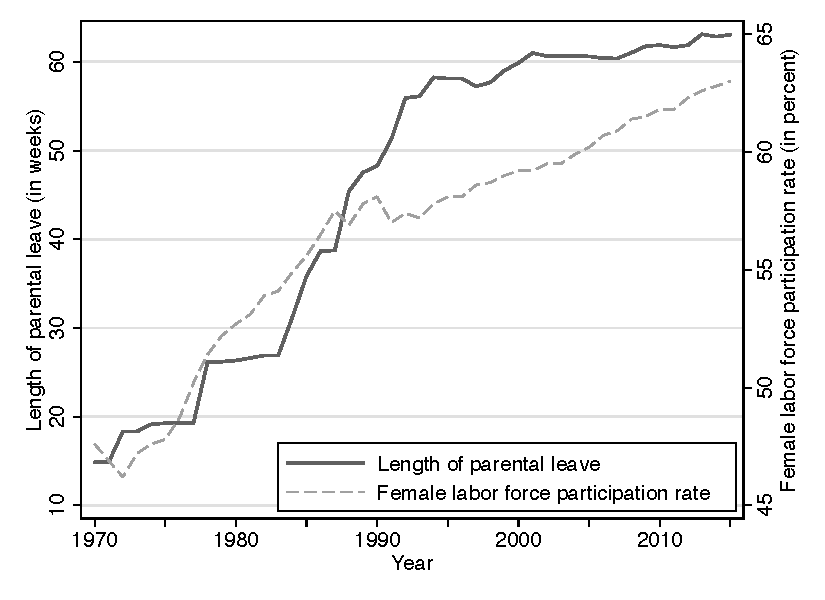
\includegraphics[width=0.9\textwidth]{../../analysis/graphs/SOEP/PL_OECD.pdf}
\caption{Average length of parental leave and female labor force participation rate across OECD countries}
\label{fig:PLOECD}
\begin{minipage}{\textwidth} % choose width suitably
{\footnotesize \textit{Note:} The lines illustrate the average length of parental leave and female labor force participation rate (women aged 15-64) across OECD countries from 1970 until 2015. The data on parental leave considers only the period of job protection, irrespective of payment conditions. \newline \textit{Source: }OECD, 
\href{http://www.oecd.org/gender/data/length-of-maternity-leave-parental-leave-and-paid-father-specific-leave.htm}{http://www.oecd.org/gender/data} and \href{https://stats.oecd.org/Index.aspx?DataSetCode=LFS_SEXAGE_I_R#}{https://stats.oecd.org/Index}\par}
\end{minipage}
\end{figure}



\begin{figure}[p]
\centering 
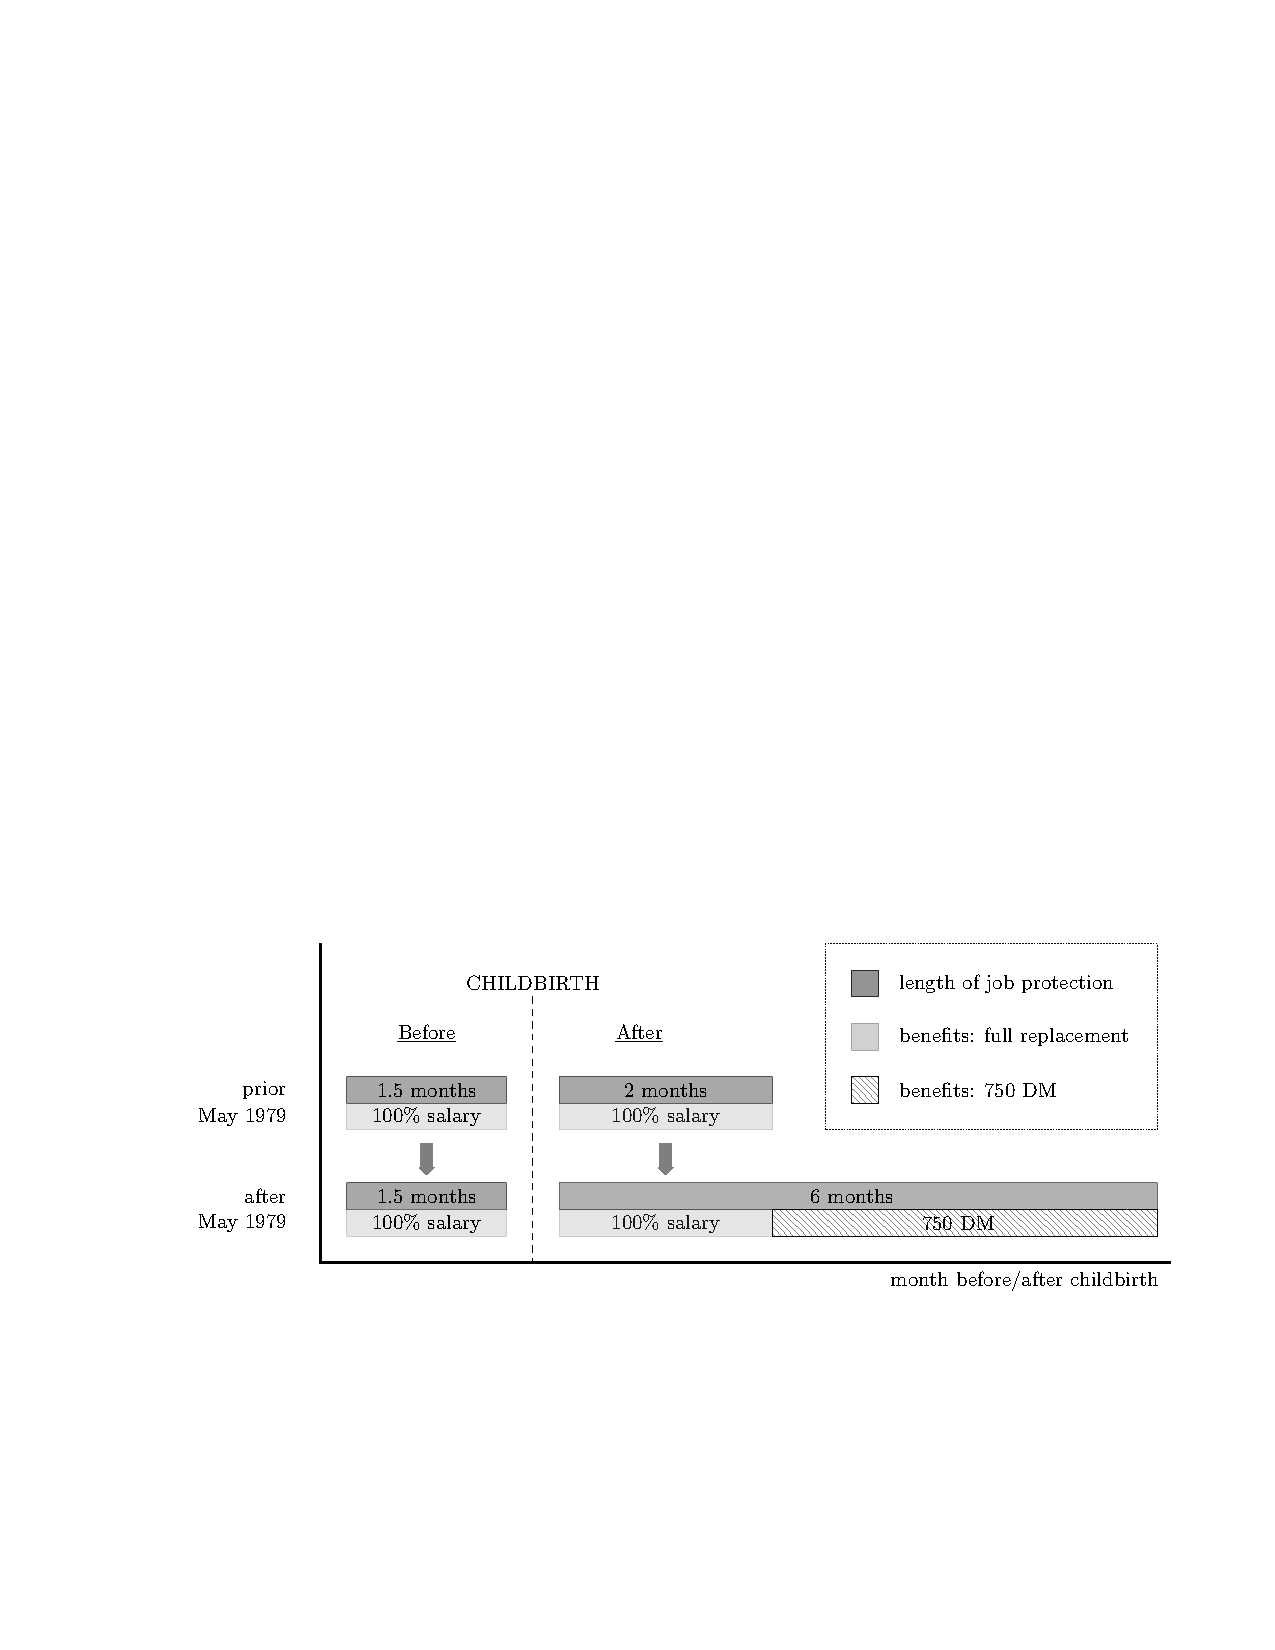
\includegraphics[width=\textwidth]{../../analysis/graphs/SOEP/reform.pdf}
\caption{1979 reform in maternity leave legislation in the Federal Republic of Germany}\label{fig: MLreform}
\begin{minipage}{\textwidth} 
{\footnotesize \textit{Note:} The figure describes a legislative change in the length of job protection and maternity leave, which took place in the Federal Republic of Germany in 1979. The reform increased post-birth maternity leave from eight weeks to six months, while keeping the initial structure of the period from six weeks before until eight weeks after childbirth unchanged.\newline \textit{Source: }The figure is based on information from \cite{dustmann2012expansions}, \cite{DIW2002}, \cite{schonberg2014expansions} as well as \cite{zmarzlik1999mutterschutzgesetz}.\par}
\end{minipage}
\end{figure}



%%%%%%%%%%%%%%%%%%%%%%%%%%%%%%%%%%%%%%%%%%%%%%%%
%		Validity
%%%%%%%%%%%%%%%%%%%%%%%%%%%%%%%%%%%%%%%%%%%%%%%%

% Fertility Histograms	

\begin{landscape} 

\begin{figure}[p]\vspace*{-2cm}
\centering
\begin{subfigure}[h]{0.7\textwidth}\centering
	\caption{Control group 1: November 1976-October 1977}
	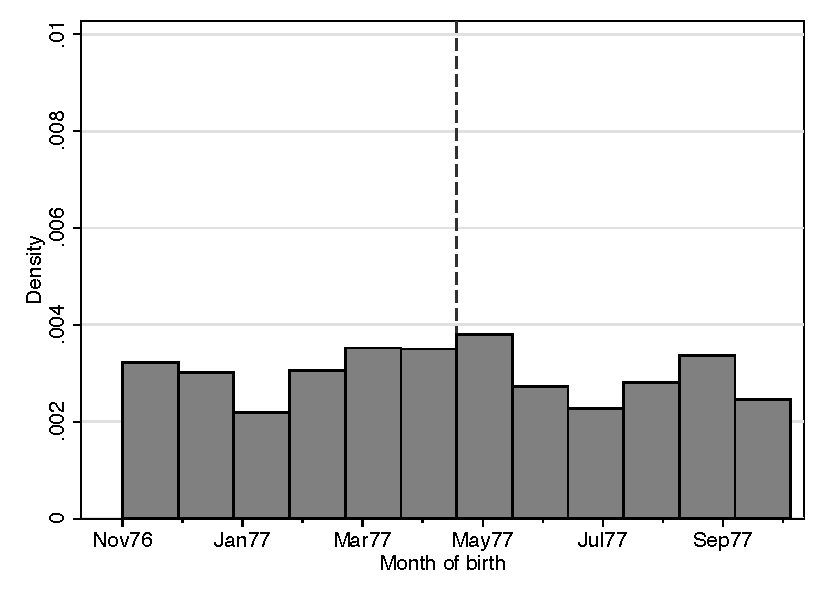
\includegraphics[width=\textwidth]{../../analysis/graphs/SOEP/fertilityhistcntrl1.pdf}
\end{subfigure}
\quad
\begin{subfigure}[h]{0.7\textwidth}\centering
	\caption{Control group 2: November 1977-October 1978}
	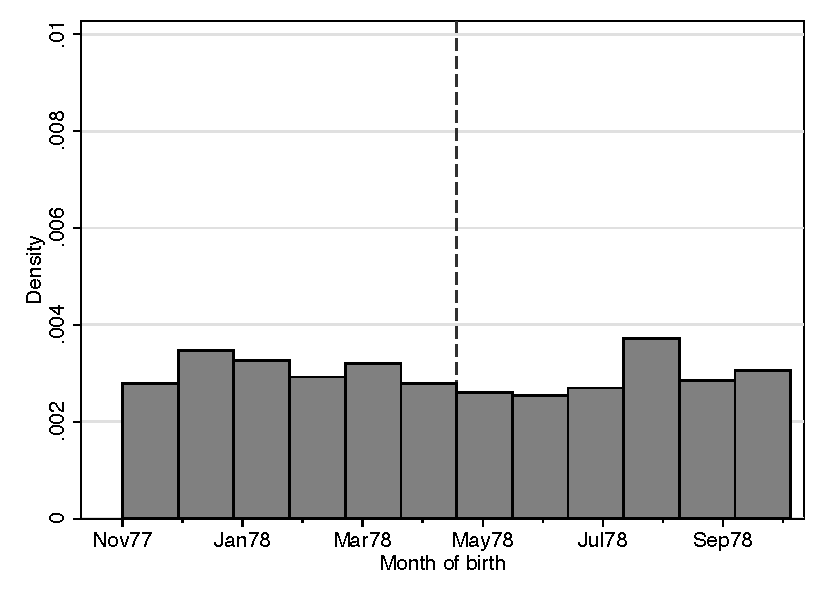
\includegraphics[width=\textwidth]{../../analysis/graphs/SOEP/fertilityhistcntrl2.pdf}
\end{subfigure}

\begin{subfigure}[h]{0.7\textwidth}\centering
	\caption{Treatment group: November 1978-October 1979}
	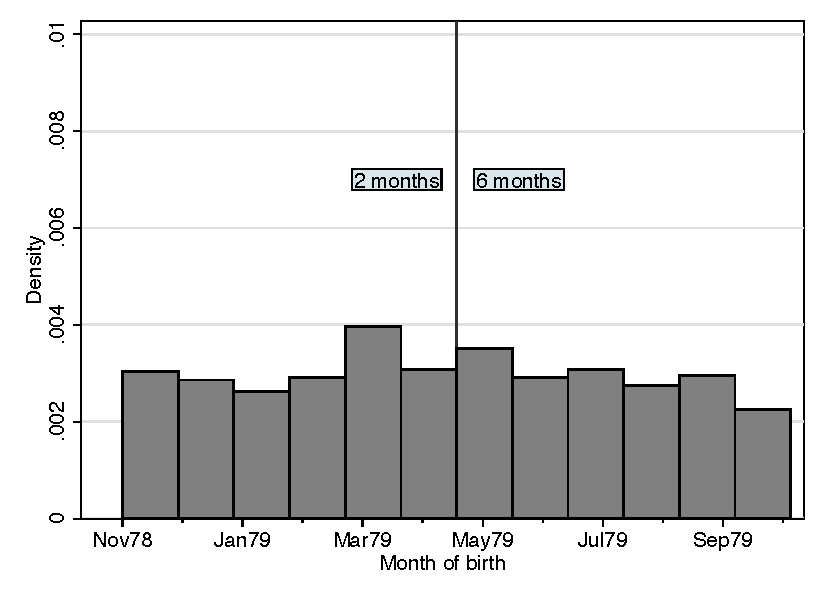
\includegraphics[width=\textwidth]{../../analysis/graphs/SOEP/fertilityhist.pdf}
\end{subfigure}
\quad
\begin{subfigure}[h]{0.7\textwidth}\centering
	\caption{Control group 3: November 1979-October 1980}
	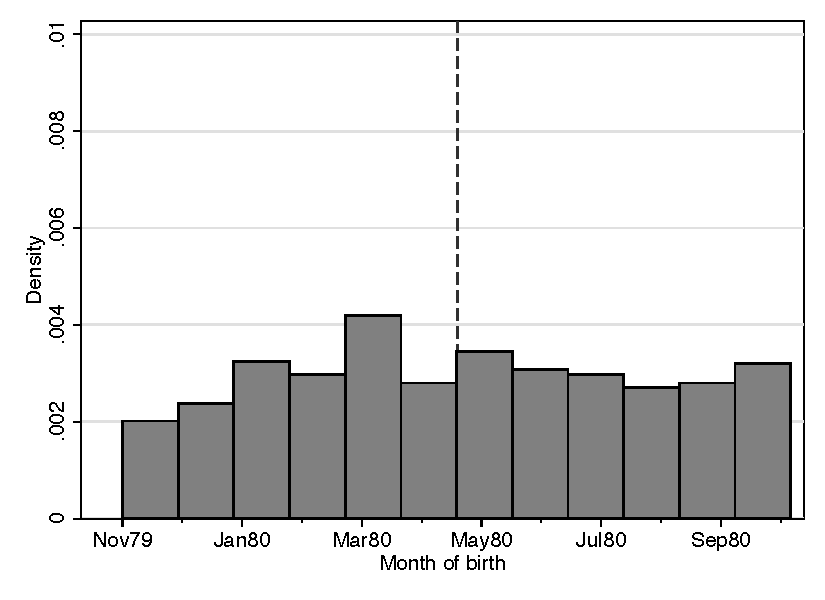
\includegraphics[width=\textwidth]{../../analysis/graphs/SOEP/fertilityhistcntrl3.pdf}
\end{subfigure}

\begin{adjustwidth}{2cm}{}
\caption{Fertility histograms for different years}\label{fig:appdx_hist}
\begin{minipage}{1.35\textwidth} % choose width suitably
{\footnotesize \textit{Note:} The histograms use one month bins. The solid vertical line divides pre- and post-reform time span for the treatment group, i.e. two or six months of job-protected leave after childbirth. The dashed lines illustrates the same cutoff value for the control groups born in other years.\newline \textit{Source: }German Socio-Economic Panel, version 31\par}
\end{minipage}
\end{adjustwidth}

\end{figure}

\end{landscape}



\clearpage
%%%%%%%%%%%%%%%
% Parental Covariate Balance






 \vspace*{\fill}
\begin{figure}[h]
	\centering
	\begin{subfigure}[t]{0.48\textwidth}
		\centering
		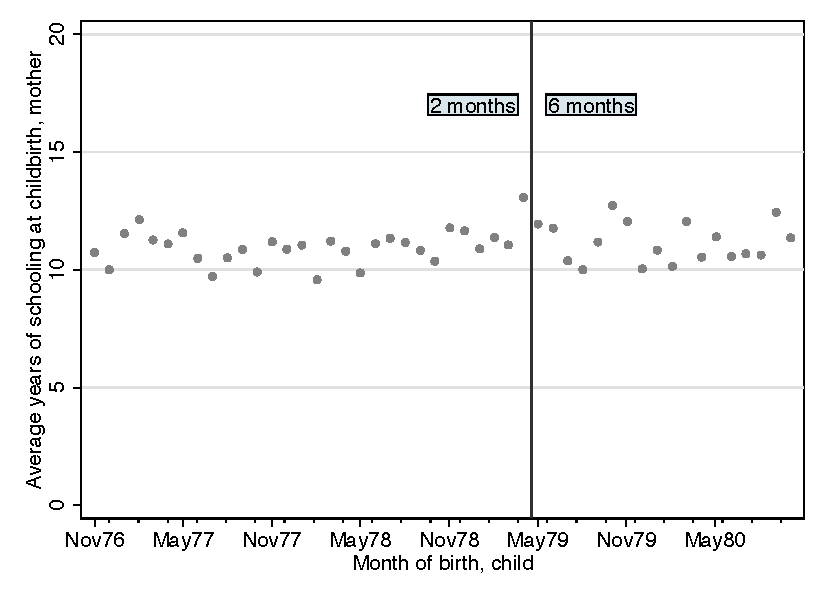
\includegraphics[width=0.99\textwidth]{../../analysis/graphs/SOEP/Meduc}
		\caption{Mothers}		
	\end{subfigure}
	\quad
	\begin{subfigure}[t]{0.48\textwidth}
		\centering
		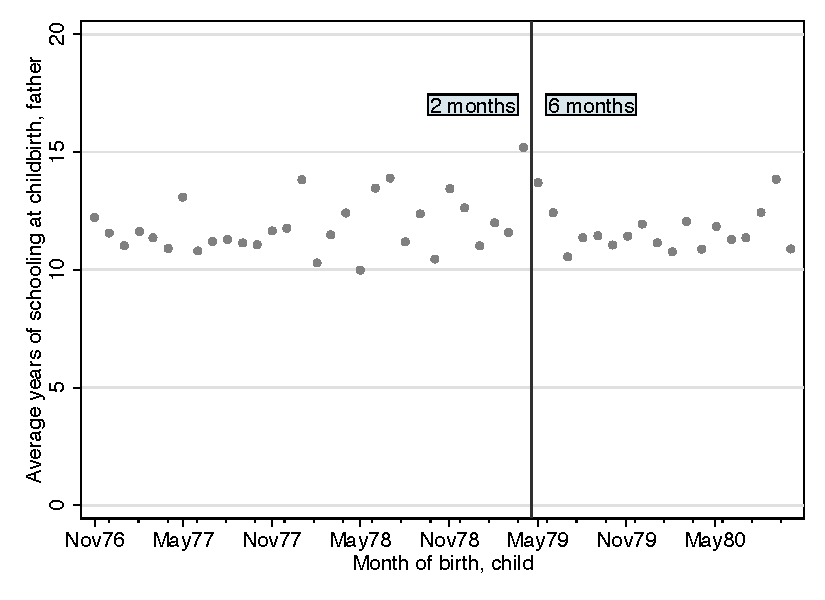
\includegraphics[width=0.99\textwidth]{../../analysis/graphs/SOEP/Feduc}
		\caption{Fathers}
	\end{subfigure}
	\caption{Average years of schooling by date of child's birth}\label{fig:yrschooling_parents_all cohorts}
	\begin{minipage}{\textwidth} % choose width suitably
{\footnotesize \textit{Note:} The averages correspond to one month bins. The solid vertical line divides pre- and post-reform time span, i.e. two or six months of job-protected maternity leave after childbirth. \newline \textit{Source: }German Socio-Economic Panel, version 31\par}
\end{minipage}
\end{figure}

\begin{figure}[h]
	\centering
	\begin{subfigure}[t]{0.48\textwidth}
		\centering
		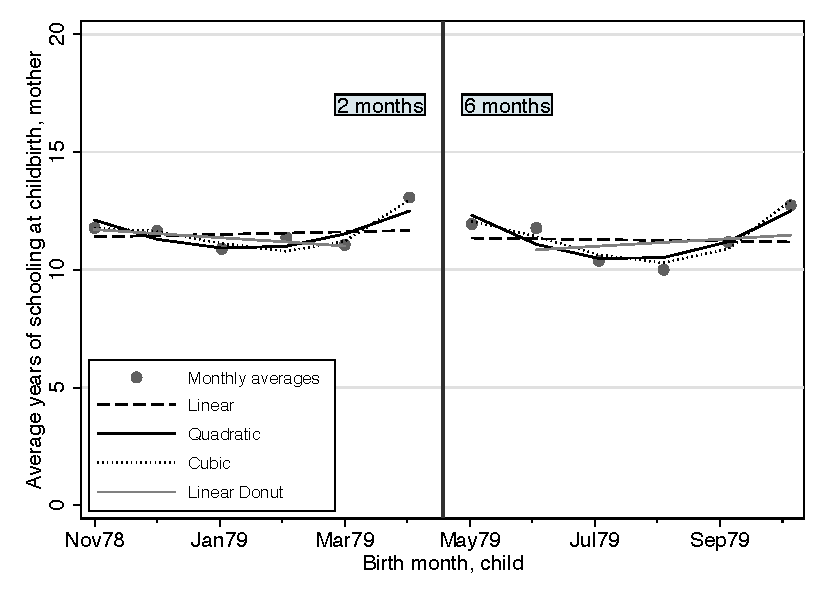
\includegraphics[width=0.99\textwidth]{../../analysis/graphs/SOEP/Meduc2}
		\caption{Mothers}		
	\end{subfigure}
	\quad
	\begin{subfigure}[t]{0.48\textwidth}
		\centering
		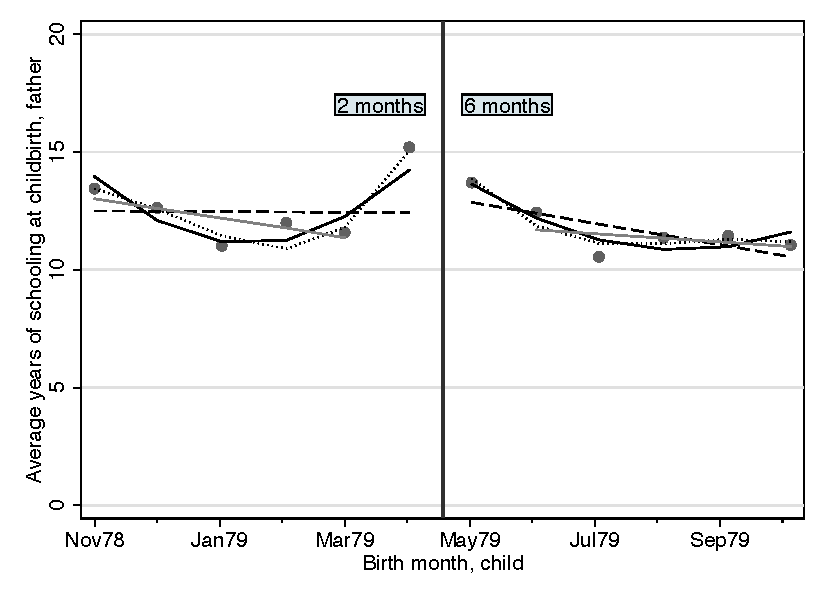
\includegraphics[width=0.99\textwidth]{../../analysis/graphs/SOEP/Feduc2}
		\caption{Fathers}
	\end{subfigure}
	\caption{Average years of schooling by date of child's birth}\label{fig:yrschooling_parents_treated cohorts}
	\begin{minipage}{\textwidth} % choose width suitably
{\footnotesize \textit{Note:} The averages correspond to one month bins. The solid vertical line divides pre- and post-reform time span, i.e. two or six months of job-protected maternity leave after childbirth. Sample only contains individuals born within half a year of the cutoff date. \newline \textit{Source: }German Socio-Economic Panel, version 31\par}
\end{minipage}
\end{figure}
\vspace*{\fill}











\clearpage

\vspace*{\fill}
\begin{figure}[h]
	\centering
	\begin{subfigure}[h]{0.48\textwidth}
		\centering
		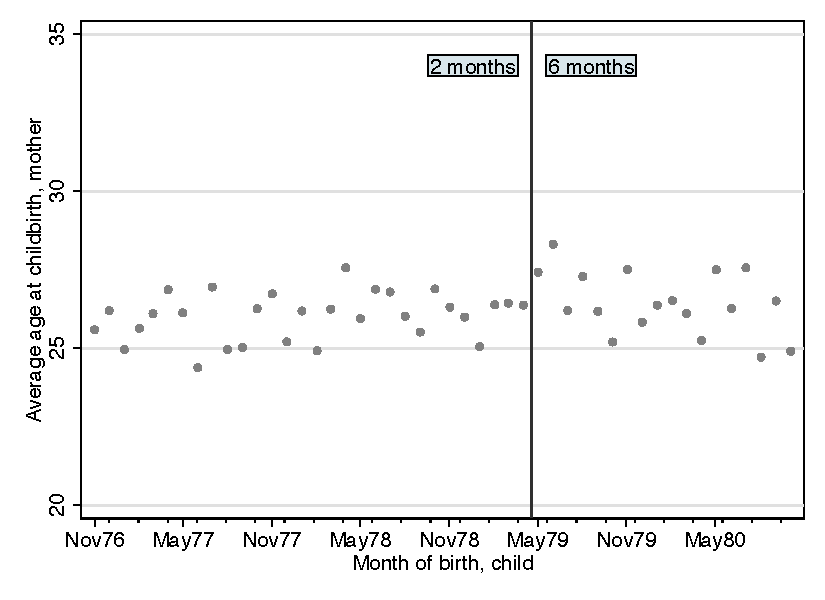
\includegraphics[width=0.99\textwidth]{../../analysis/graphs/SOEP/Magebirth2}
		\caption{Mothers}		
	\end{subfigure}
	\quad
	\begin{subfigure}[h]{0.48\textwidth}
		\centering
		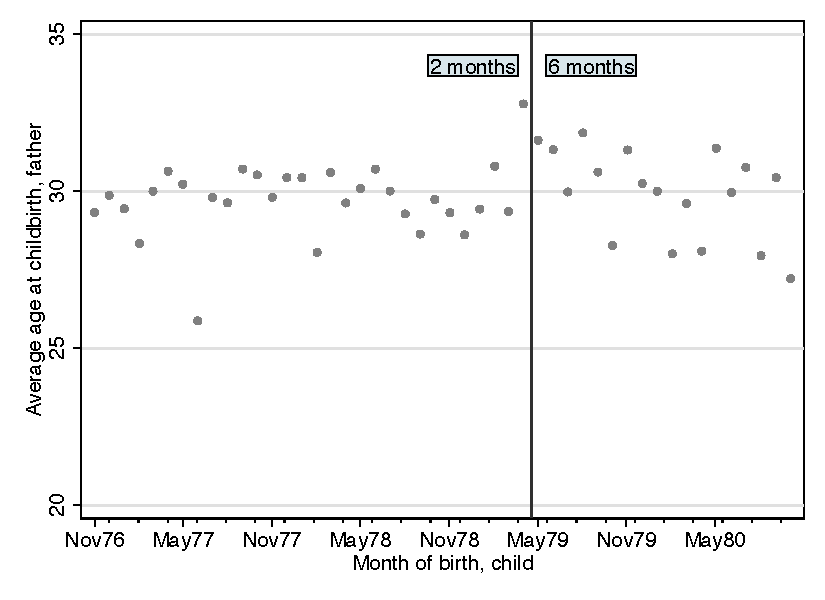
\includegraphics[width=0.99\textwidth]{../../analysis/graphs/SOEP/Fagebirth2}
		\caption{Fathers}
	\end{subfigure}
	\caption{Average age by date of child's birth}\label{fig:age_birth_all cohorts}
	\begin{minipage}{\textwidth} % choose width suitably
{\footnotesize \textit{Note:} The averages correspond to one month bins. The solid vertical line divides pre- and post-reform time span, i.e. two or six months of job-protected maternity leave after childbirth. \newline \textit{Source: }German Socio-Economic Panel, version 31\par}
\end{minipage}
\end{figure}

\begin{figure}[h]
	\centering
	\begin{subfigure}[h]{0.48\textwidth}
		\centering
		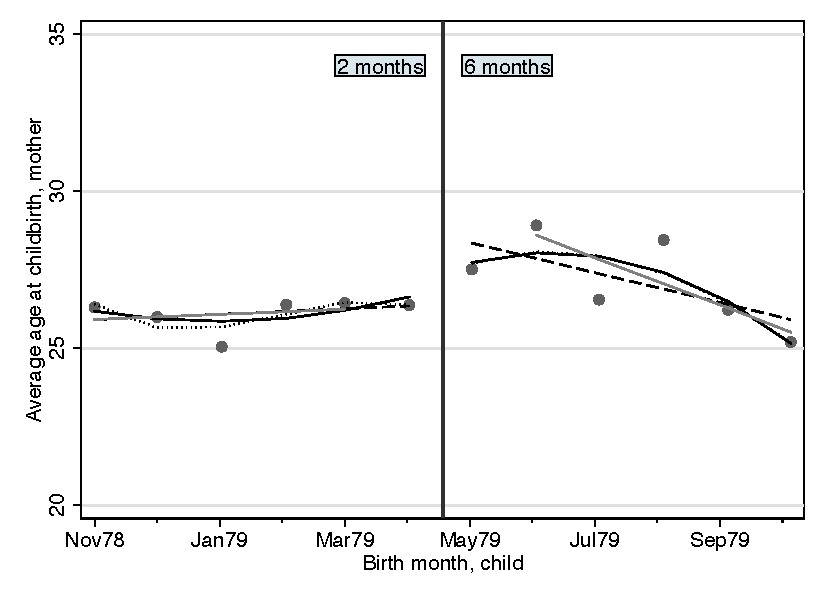
\includegraphics[width=0.99\textwidth]{../../analysis/graphs/SOEP/Magebirth2_treated}
		\caption{Mothers}		
	\end{subfigure}
	\quad
	\begin{subfigure}[h]{0.48\textwidth}
		\centering
		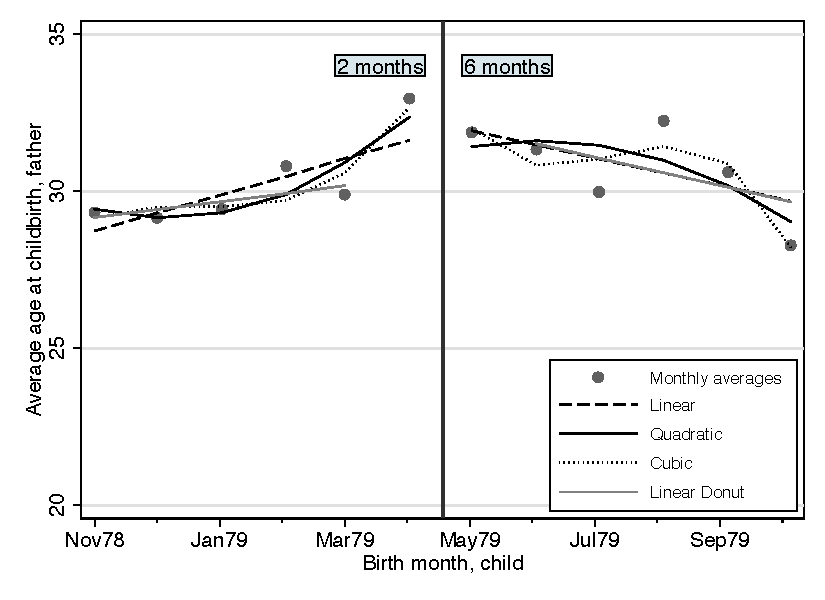
\includegraphics[width=0.99\textwidth]{../../analysis/graphs/SOEP/Fagebirth2_treated}
		\caption{Fathers}
	\end{subfigure}
	\caption{Average age by date of child's birth}\label{fig:age_birth_treatment cohort}
	\begin{minipage}{\textwidth} % choose width suitably
{\footnotesize \textit{Note:} The averages correspond to one month bins. The solid vertical line divides pre- and post-reform time span, i.e. two or six months of job-protected maternity leave after childbirth. Sample only contains individual born within half a year of the cutoff date. \newline \textit{Source: }German Socio-Economic Panel, version 31\par}
\end{minipage}
\end{figure}
\vspace*{\fill}

%%%%%%%%%%%%%%%
% PARENTAL NATIONALITY
\newpage
\vspace*{\fill}
\begin{figure}[h]
	\centering
	\begin{subfigure}[h]{0.48\textwidth}
		\centering
		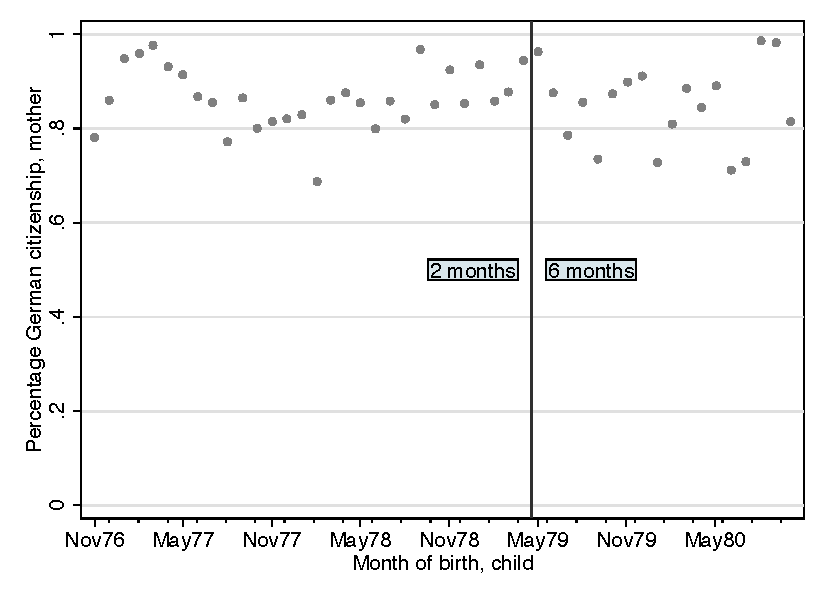
\includegraphics[width=0.99\textwidth]{../../analysis/graphs/SOEP/D_mcitizen.pdf}
		\caption{Mothers}		
	\end{subfigure}
	\quad
	\begin{subfigure}[h]{0.48\textwidth}
		\centering
		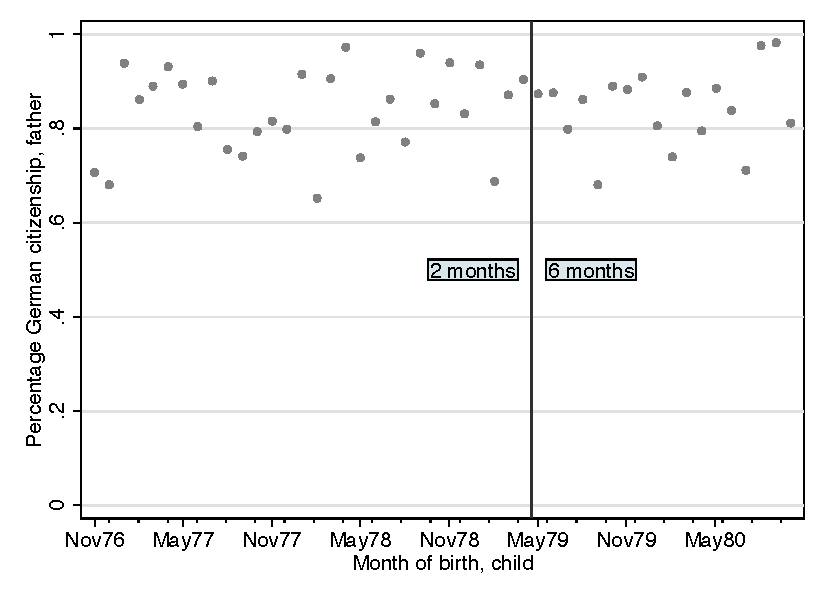
\includegraphics[width=0.99\textwidth]{../../analysis/graphs/SOEP/D_fcitizen.pdf}
		\caption{Fathers}
	\end{subfigure}
	\caption{Percentage German citizenship by date of child's birth}\label{fig:citizen_all cohorts}
	\begin{minipage}{\textwidth} % choose width suitably
{\footnotesize \textit{Note:} The averages correspond to one month bins. The solid vertical line divides pre- and post-reform time span, i.e. two or six months of job-protected maternity leave after childbirth. \newline \textit{Source: }German Socio-Economic Panel, version 31\par}
\end{minipage}
\end{figure}

\begin{figure}[h]
	\centering
	\begin{subfigure}[h]{0.48\textwidth}
		\centering
		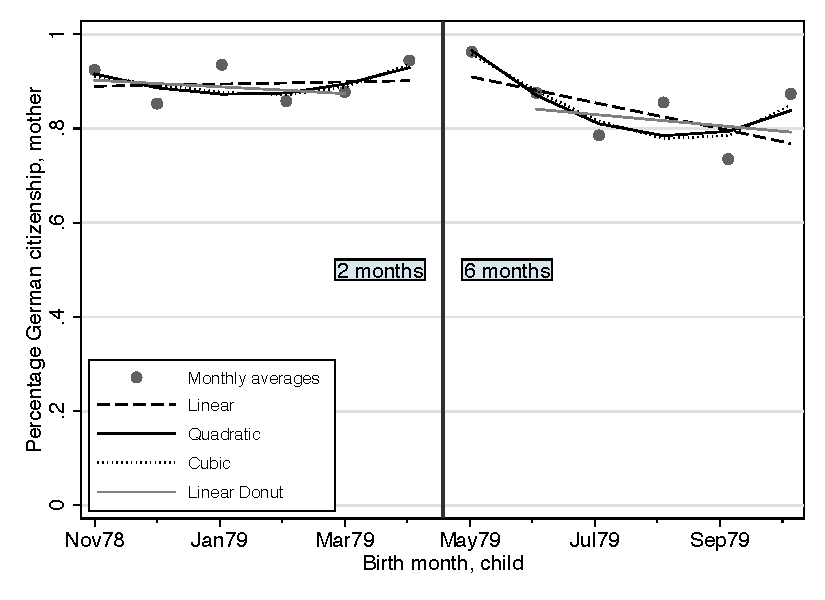
\includegraphics[width=0.99\textwidth]{../../analysis/graphs/SOEP/D_mcitizen_treated}
		\caption{Mothers}		
	\end{subfigure}
	\quad
	\begin{subfigure}[h]{0.48\textwidth}
		\centering
		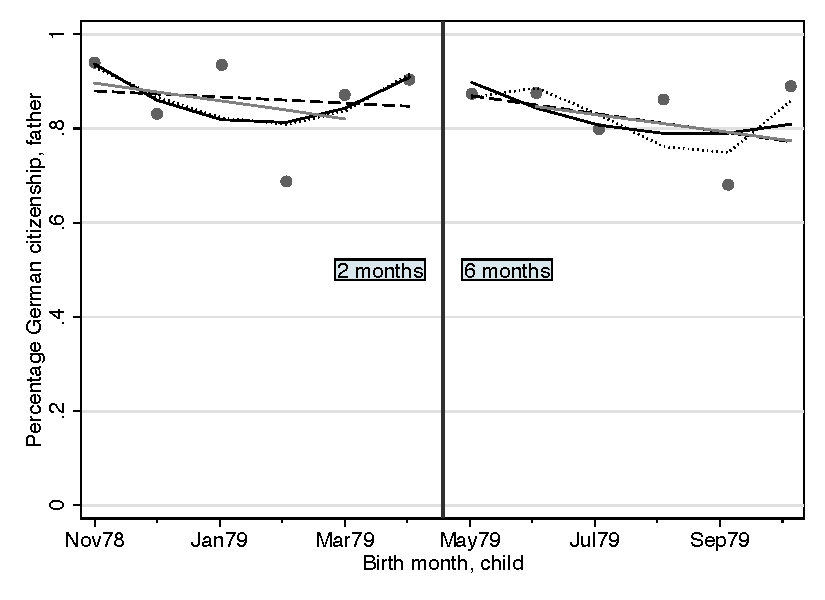
\includegraphics[width=0.99\textwidth]{../../analysis/graphs/SOEP/D_fcitizen_treated}
		\caption{Fathers}
	\end{subfigure}
	\caption{Percentage German citizenship by date of child's birth}\label{fig:citizen_treatment cohort}
	\begin{minipage}{\textwidth} % choose width suitably
{\footnotesize \textit{Note:} The averages correspond to one month bins. The solid vertical line divides pre- and post-reform time span, i.e. two or six months of job-protected maternity leave after childbirth. Sample only contains individual born within half a year of the cutoff date. \newline \textit{Source: }German Socio-Economic Panel, version 31\par}
\end{minipage}
\end{figure}
\vspace*{\fill}




\clearpage
%%%%%%%%%%%%%%%%%%%%%%%%%%%%%%%%%%%%%%%%%%%%%%%%
%		Regression Discontinuity graphs
%%%%%%%%%%%%%%%%%%%%%%%%%%%%%%%%%%%%%%%%%%%%%%%%
%		 BM
\newpage
\begin{figure}[p]
\begin{subfigure}[h]{0.48\textwidth}\centering
	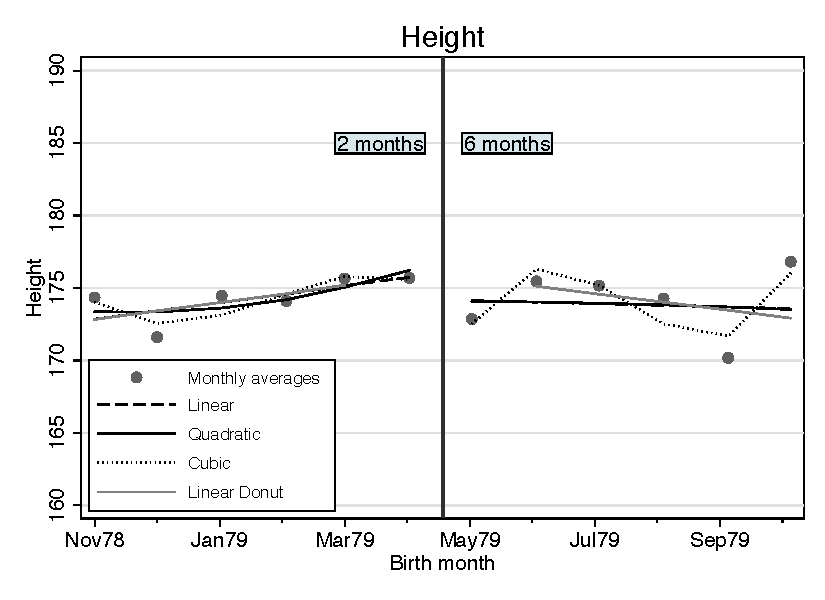
\includegraphics[width=\textwidth]{../../analysis/graphs/SOEP/Height_RD.pdf}
\end{subfigure}
\quad
\begin{subfigure}[h]{0.48\textwidth}\centering
	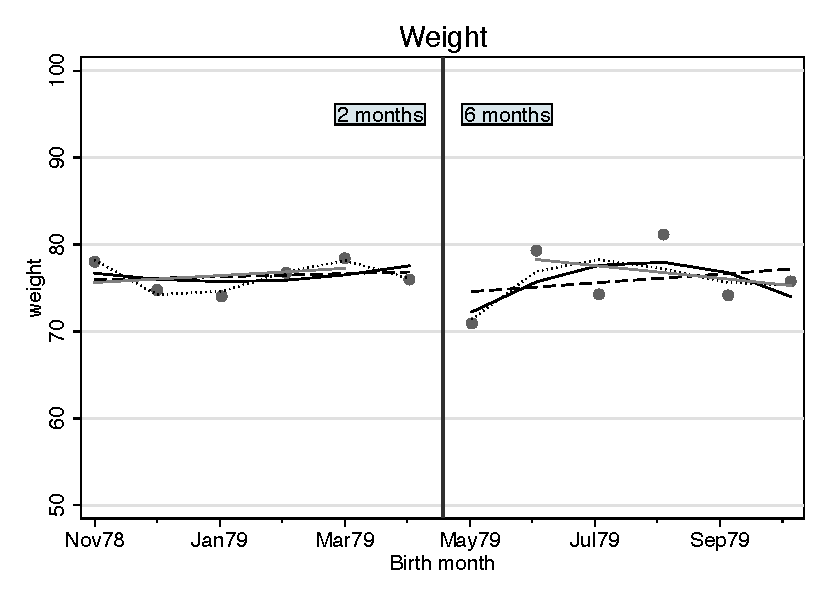
\includegraphics[width=\textwidth]{../../analysis/graphs/SOEP/Weight_RD.pdf}
\end{subfigure}

\begin{subfigure}[h]{0.48\textwidth}\centering
	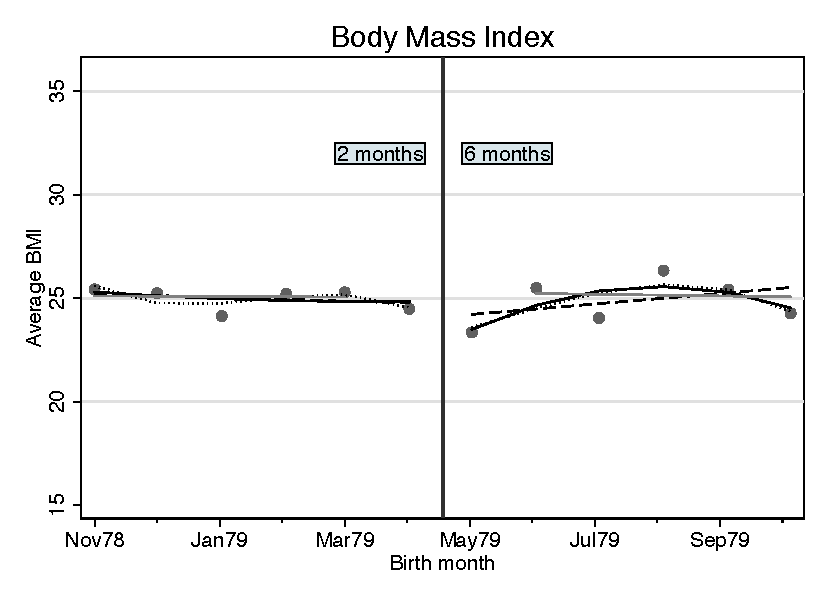
\includegraphics[width=\textwidth]{../../analysis/graphs/SOEP/BMI_RD.pdf}
\end{subfigure}
\quad
\begin{subfigure}[h]{0.48\textwidth}\centering
	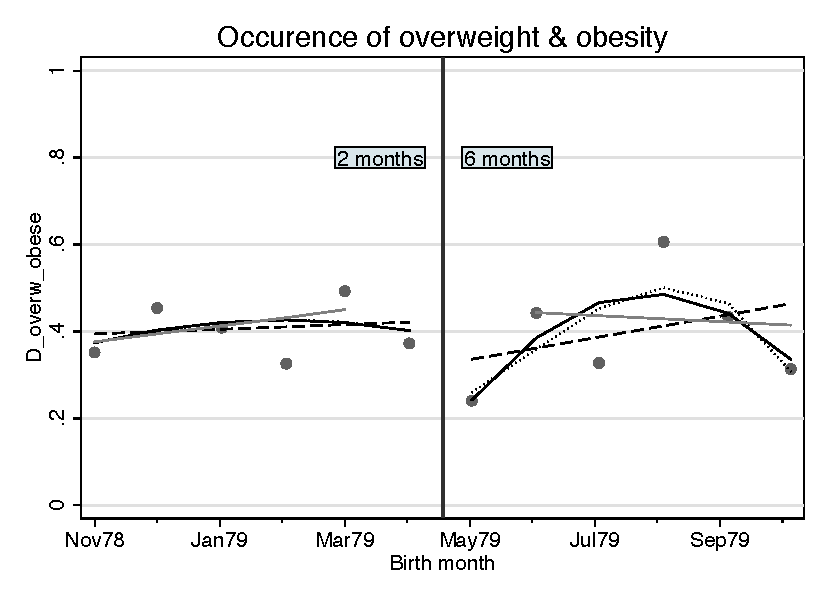
\includegraphics[width=\textwidth]{../../analysis/graphs/SOEP/D_overw_obese_RD.pdf}
\end{subfigure}
\caption{Impact of 1979 maternity leave expansion on biometric outcomes}\label{fig: RD_BM}
\begin{minipage}{\textwidth} % choose width suitably
{\footnotesize \textit{Note:} The averages correspond to one month bins. The solid vertical line divides pre- and post-reform time span, i.e. two or six months of job-protected leave after childbirth. Sample only contains individual born within half a year of the cutoff date. \newline \textit{Source: }German Socio-Economic Panel, version 31\par}
\end{minipage}
\end{figure}
%		 OH
\newpage
\begin{figure}[p]
\begin{subfigure}[h]{0.48\textwidth}\centering
	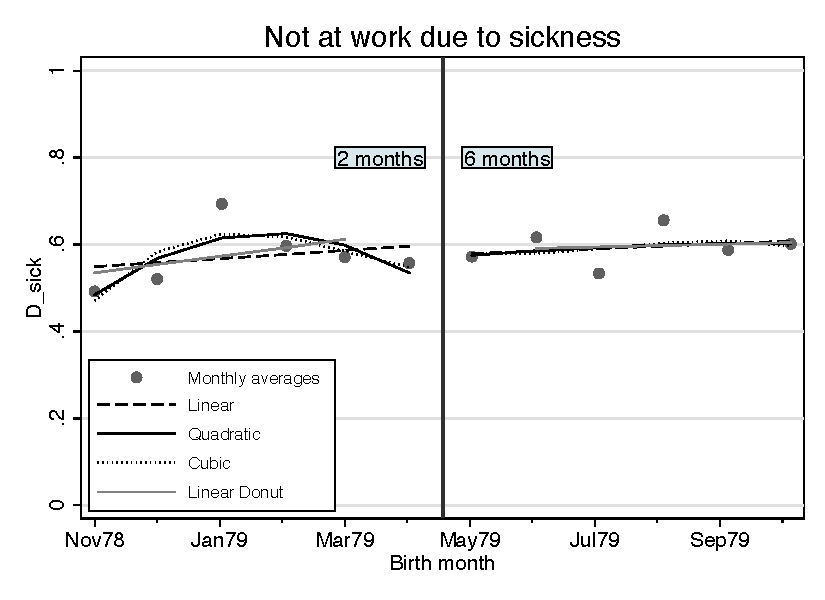
\includegraphics[width=\textwidth]{../../analysis/graphs/SOEP/D_sick_RD.pdf}
\end{subfigure}
\quad
\begin{subfigure}[h]{0.48\textwidth}\centering
	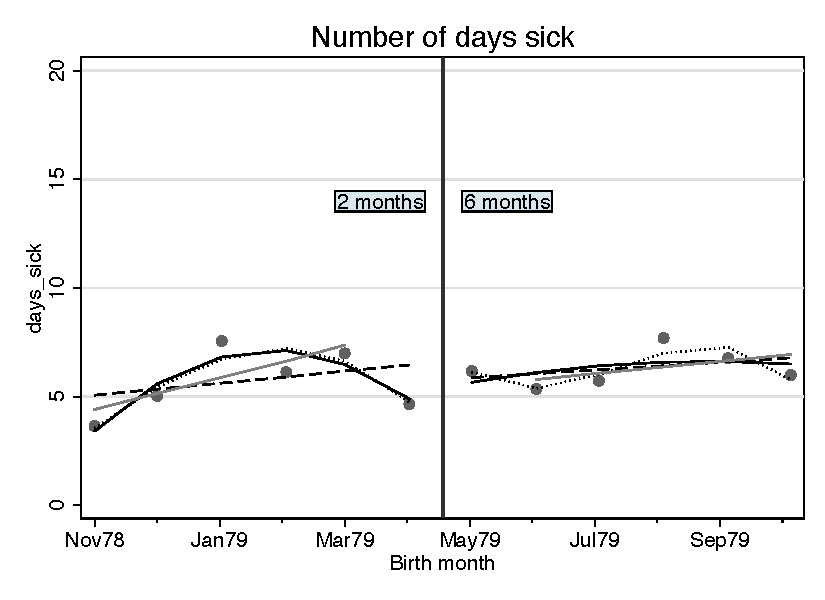
\includegraphics[width=\textwidth]{../../analysis/graphs/SOEP/Days_sick_RD.pdf}
\end{subfigure}

\begin{subfigure}[h]{0.48\textwidth}\centering
	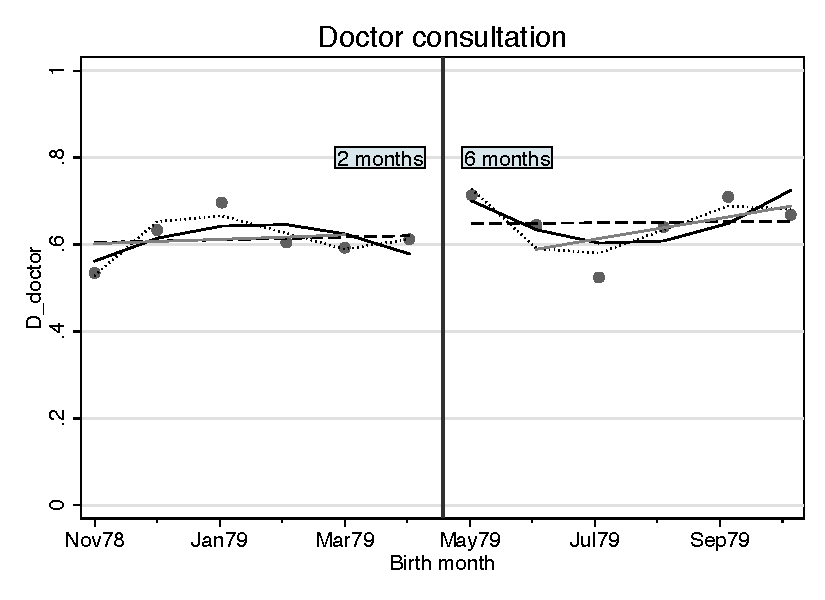
\includegraphics[width=\textwidth]{../../analysis/graphs/SOEP/D_doctor_RD.pdf}
\end{subfigure}
\quad
\begin{subfigure}[h]{0.48\textwidth}\centering
	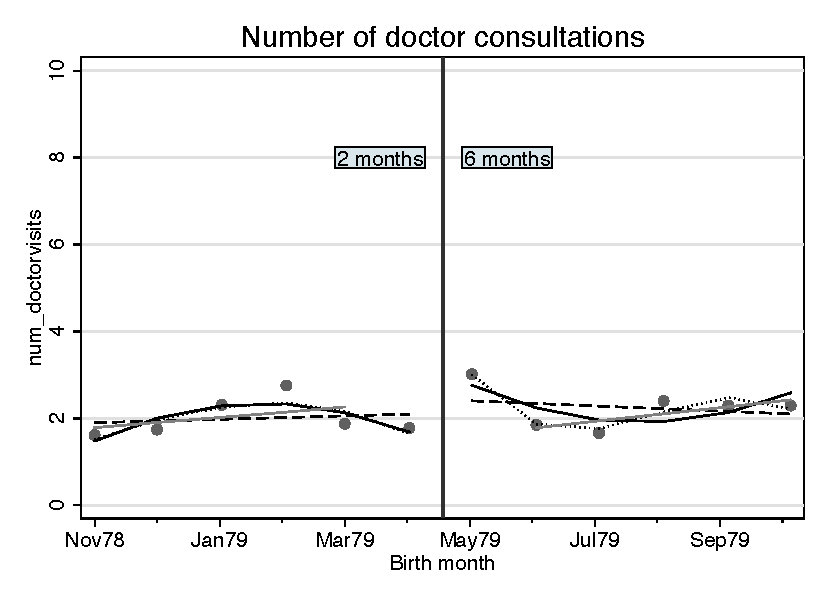
\includegraphics[width=\textwidth]{../../analysis/graphs/SOEP/Docvisits_RD.pdf}
\end{subfigure}



\begin{subfigure}[h]{0.48\textwidth}\centering
	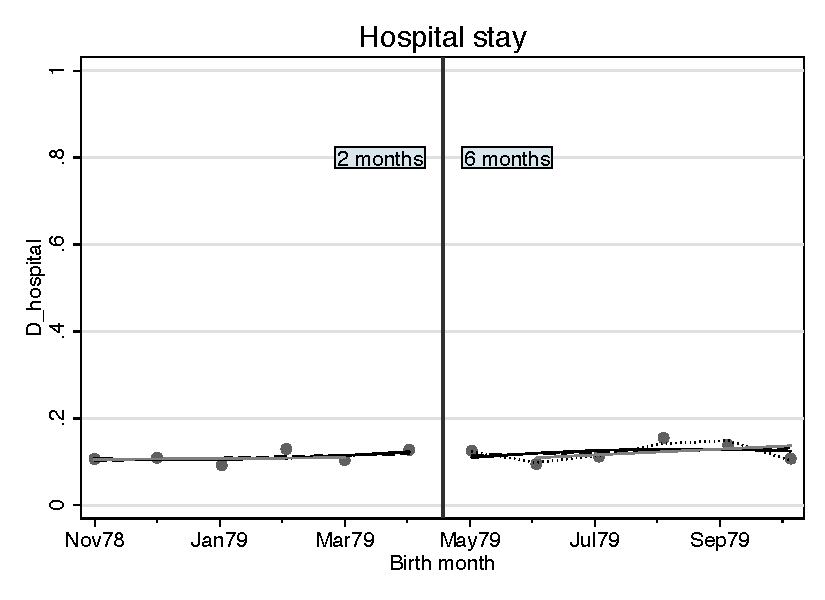
\includegraphics[width=\textwidth]{../../analysis/graphs/SOEP/D_hospital_RD.pdf}
\end{subfigure}
\quad
\begin{subfigure}[h]{0.48\textwidth}\centering
	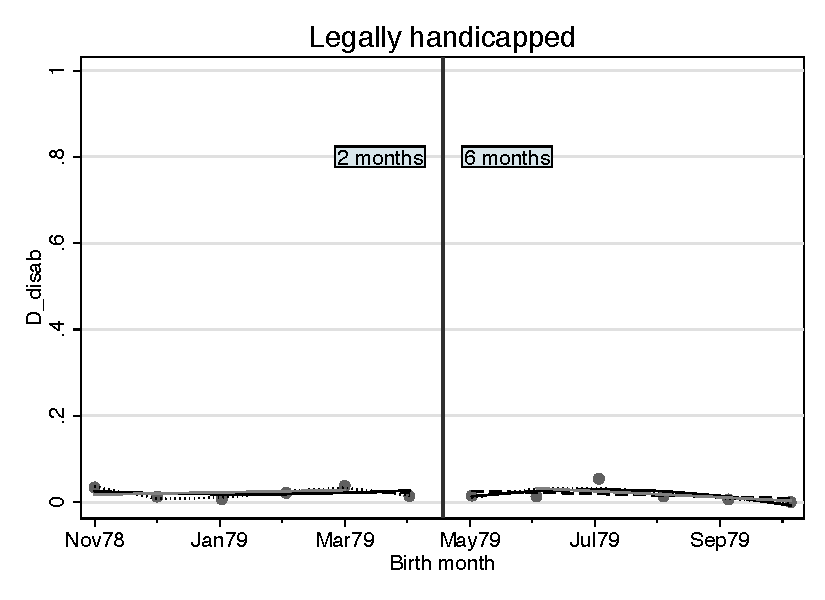
\includegraphics[width=\textwidth]{../../analysis/graphs/SOEP/D_disab_RD.pdf}
\end{subfigure}

\begin{subfigure}[h]{0.48\textwidth}\centering
	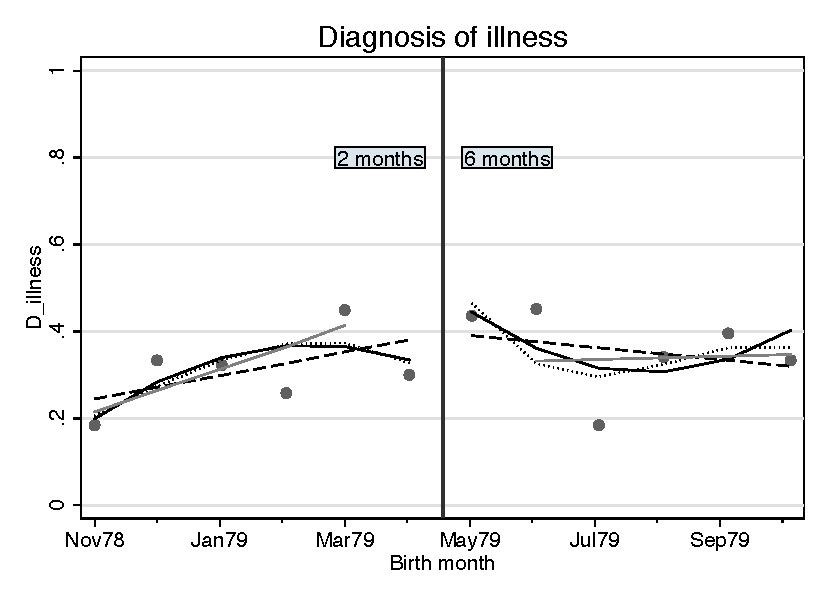
\includegraphics[width=\textwidth]{../../analysis/graphs/SOEP/D_illness_RD.pdf}
\end{subfigure}
\quad
\begin{subfigure}[h]{0.48\textwidth}\centering
	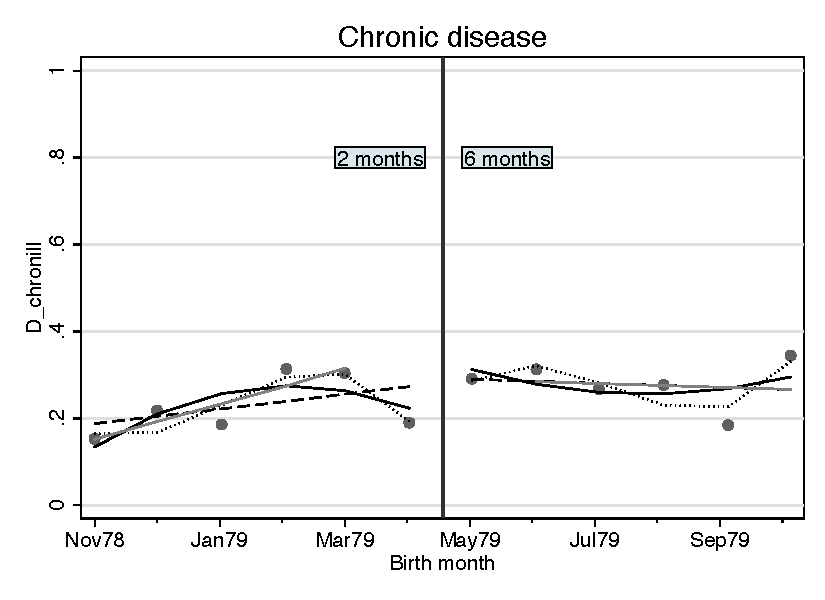
\includegraphics[width=\textwidth]{../../analysis/graphs/SOEP/D_chronill_RD.pdf}
\end{subfigure}

\caption{Impact of 1979 maternity leave expansion on objective health outcomes}\label{fig: RD_OH}
\begin{minipage}{\textwidth} % choose width suitably
{\footnotesize \textit{Note:} The averages correspond to one month bins. The solid vertical line divides pre- and post-reform time span, i.e. two or six months of job-protected leave after childbirth. Sample only contains individual born within half a year of the cutoff date. \newline \textit{Source: }German Socio-Economic Panel, version 31\par}
\end{minipage}
\end{figure}
% 		SH
\newpage
\begin{figure}[p]
\begin{subfigure}[h]{0.48\textwidth}\centering
	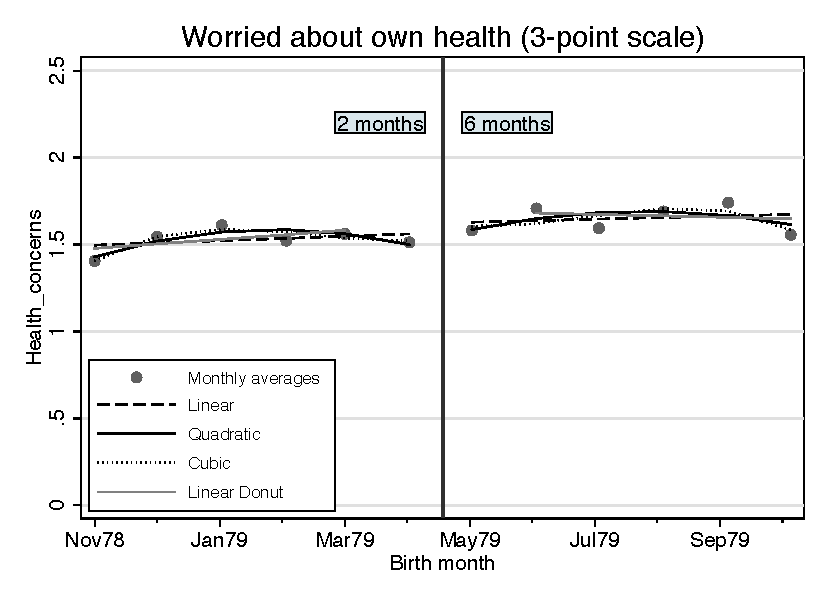
\includegraphics[width=\textwidth]{../../analysis/graphs/SOEP/Health_concerns_RD.pdf}
\end{subfigure}
\quad
\begin{subfigure}[h]{0.48\textwidth}\centering
	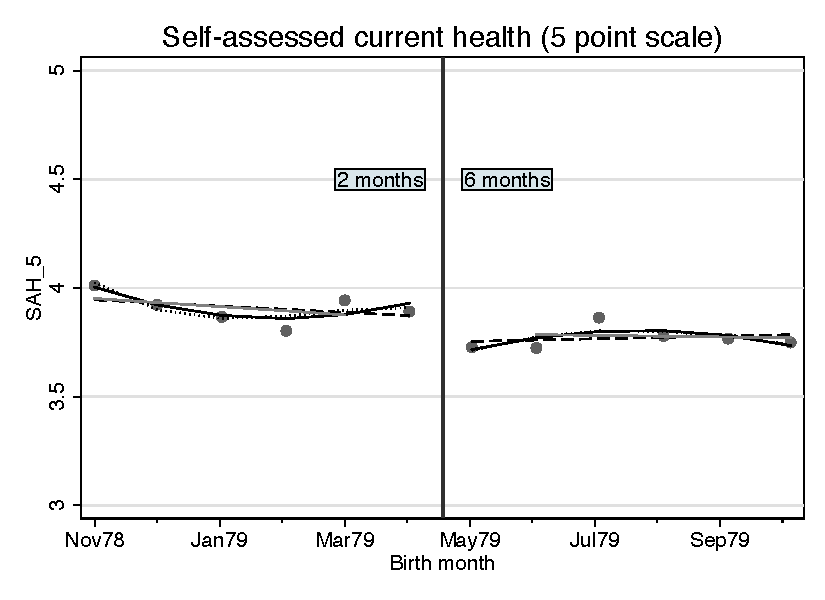
\includegraphics[width=\textwidth]{../../analysis/graphs/SOEP/SAH_5_RD.pdf}
\end{subfigure}

\begin{subfigure}[h]{0.48\textwidth}\centering
	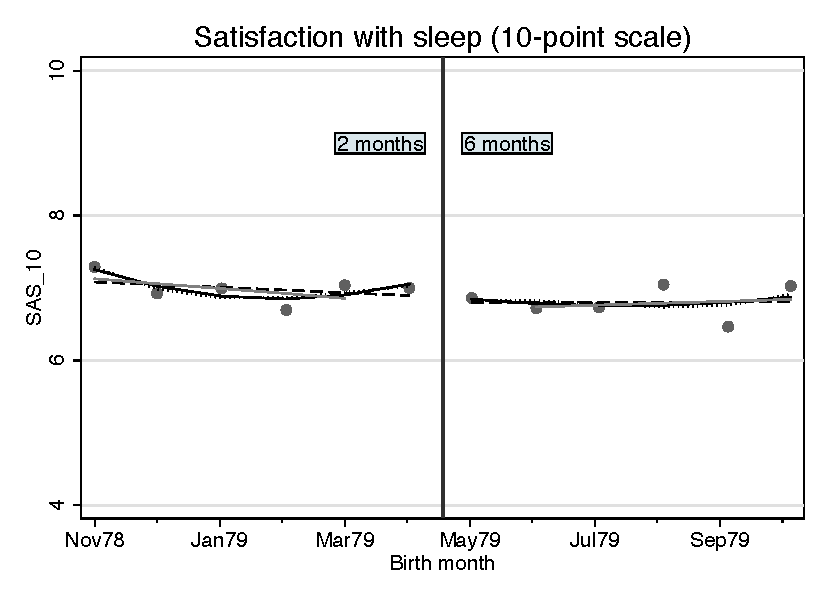
\includegraphics[width=\textwidth]{../../analysis/graphs/SOEP/SAS_10_RD.pdf}
\end{subfigure}
\quad
\begin{subfigure}[h]{0.48\textwidth}\centering
	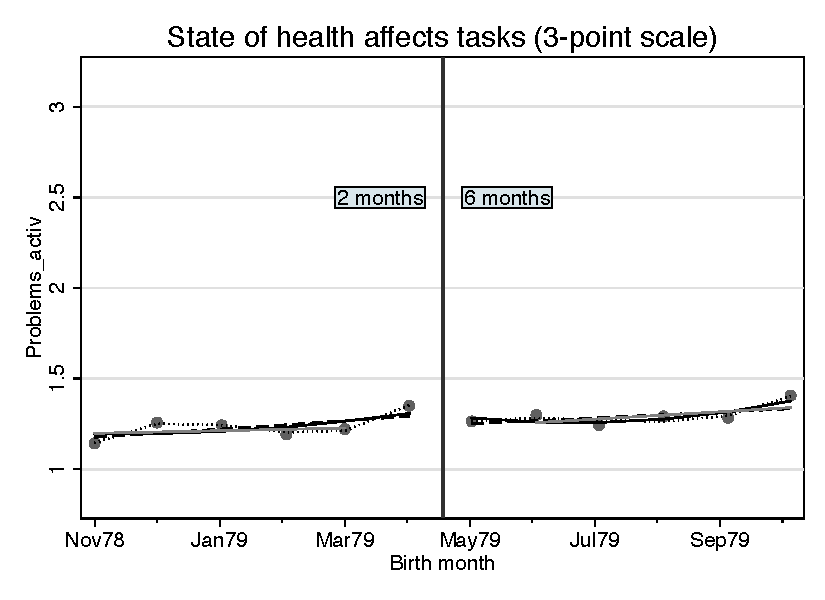
\includegraphics[width=\textwidth]{../../analysis/graphs/SOEP/Problems_activ_RD.pdf}
\end{subfigure}



\begin{subfigure}[h]{0.48\textwidth}\centering
	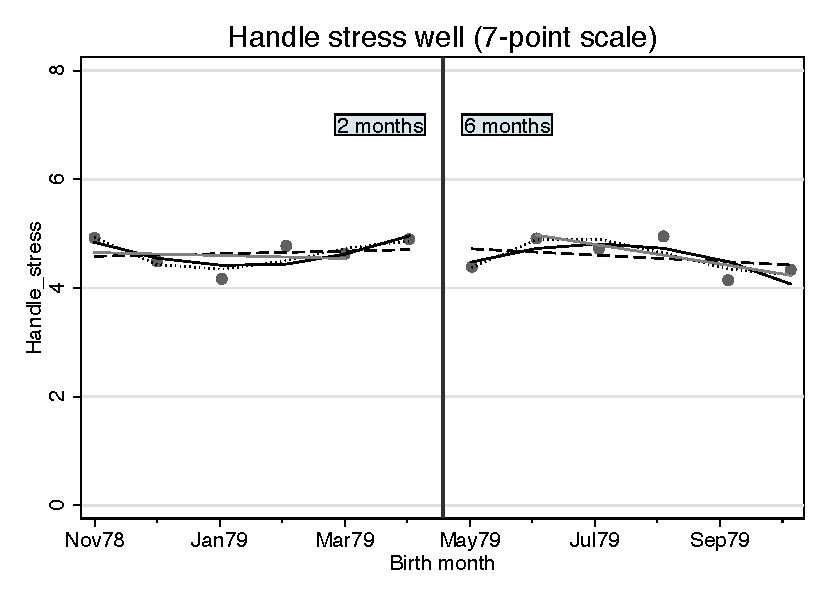
\includegraphics[width=\textwidth]{../../analysis/graphs/SOEP/Handle_stress_RD.pdf}
\end{subfigure}
\quad
\begin{subfigure}[h]{0.48\textwidth}\centering
	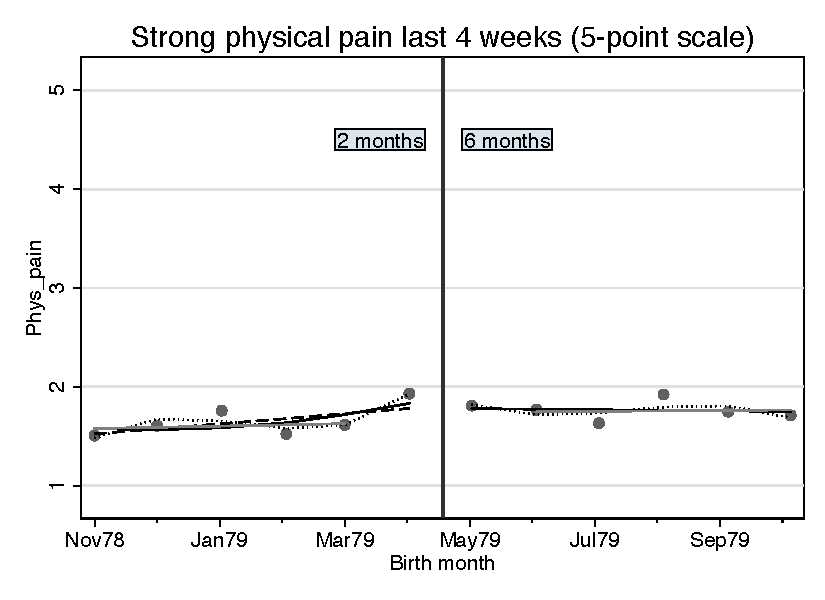
\includegraphics[width=\textwidth]{../../analysis/graphs/SOEP/Phys_pain_RD.pdf}
\end{subfigure}

\begin{subfigure}[h]{0.48\textwidth}\centering
	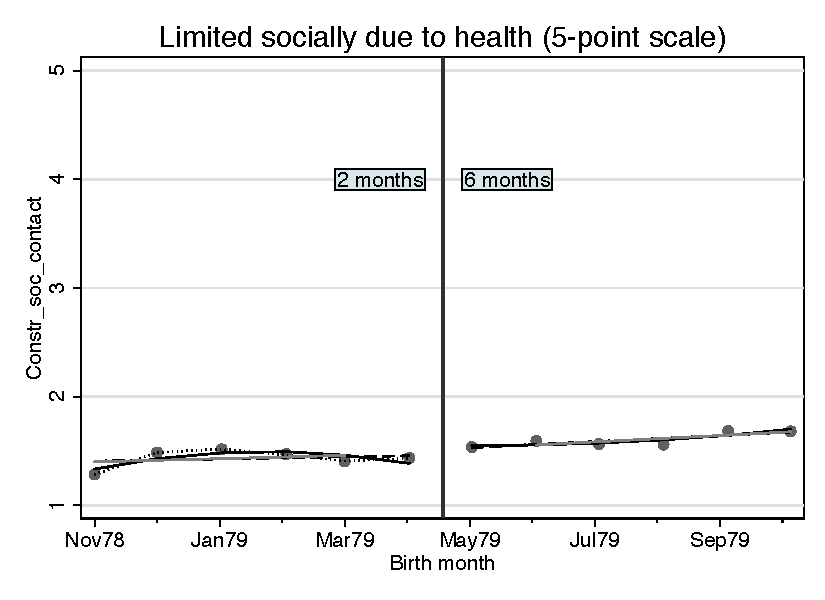
\includegraphics[width=\textwidth]{../../analysis/graphs/SOEP/Constr_soc_contact_RD.pdf}
\end{subfigure}


\caption{Impact of 1979 maternity leave expansion on subjective health outcomes}\label{fig: RD_SH}
\begin{minipage}{\textwidth} % choose width suitably
{\footnotesize \textit{Note:} The averages correspond to one month bins. The solid vertical line divides pre- and post-reform time span, i.e. two or six months of job-protected leave after childbirth. Sample only contains individual born within half a year of the cutoff date. \newline \textit{Source: }German Socio-Economic Panel, version 31\par}
\end{minipage}
\end{figure}

%		 HB
\newpage
\begin{figure}[p]
\begin{subfigure}[h]{0.48\textwidth}\centering
	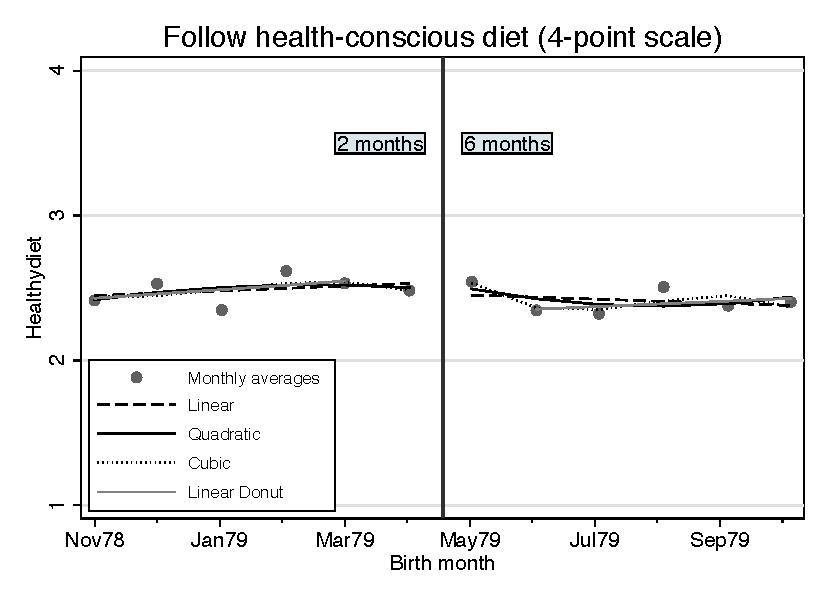
\includegraphics[width=\textwidth]{../../analysis/graphs/SOEP/Healthydiet_RD.pdf}
\end{subfigure}
\quad
\begin{subfigure}[h]{0.48\textwidth}\centering
	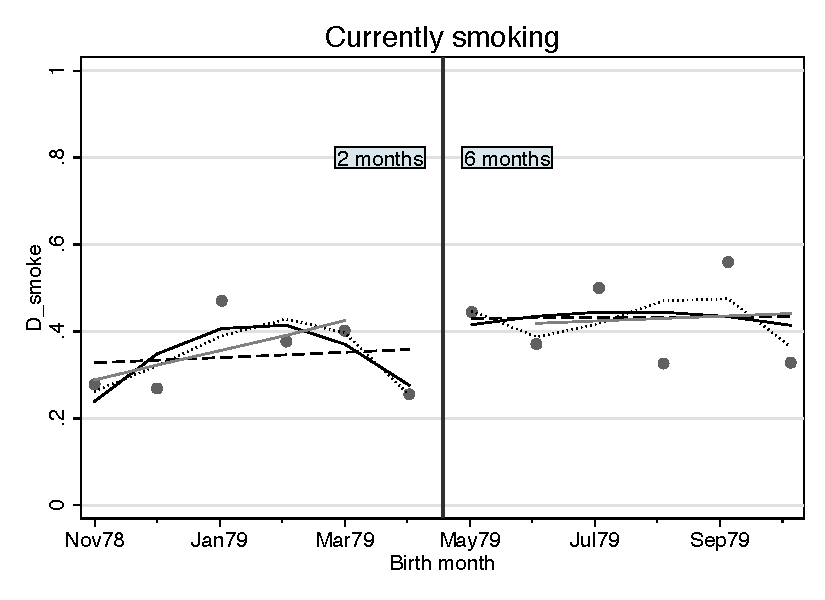
\includegraphics[width=\textwidth]{../../analysis/graphs/SOEP/D_smoke_RD.pdf}
\end{subfigure}

\begin{subfigure}[h]{0.48\textwidth}\centering
	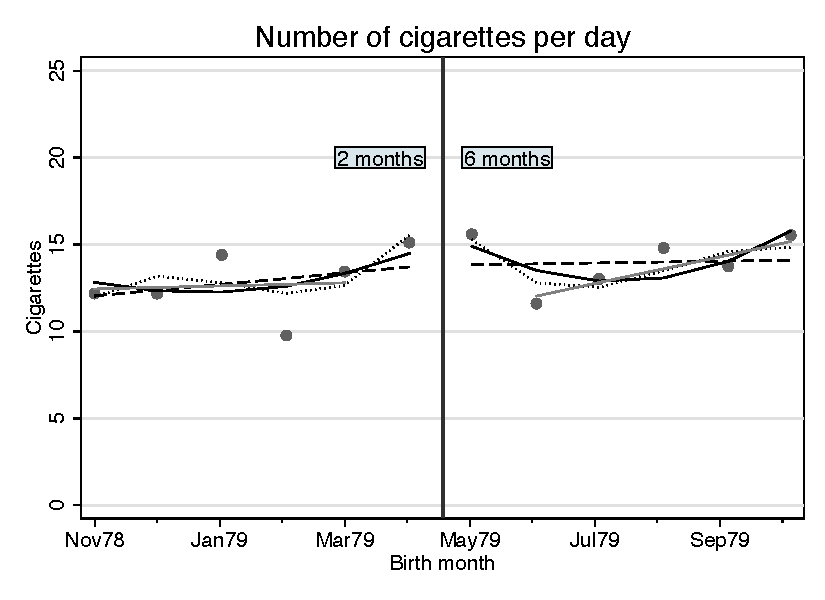
\includegraphics[width=\textwidth]{../../analysis/graphs/SOEP/Cigarettes_RD.pdf}
\end{subfigure}
\quad
\begin{subfigure}[h]{0.48\textwidth}\centering
	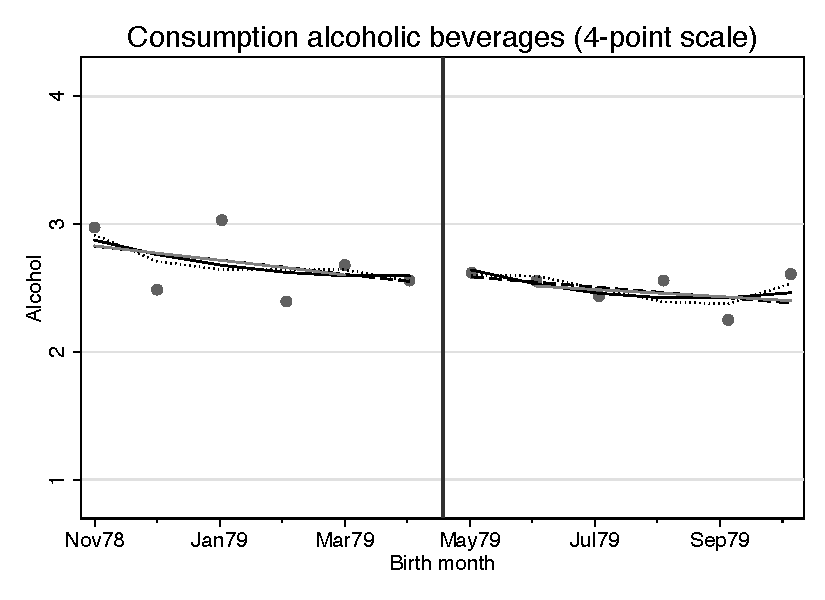
\includegraphics[width=\textwidth]{../../analysis/graphs/SOEP/Alcohol_RD.pdf}
\end{subfigure}



\begin{subfigure}[h]{0.48\textwidth}\centering
	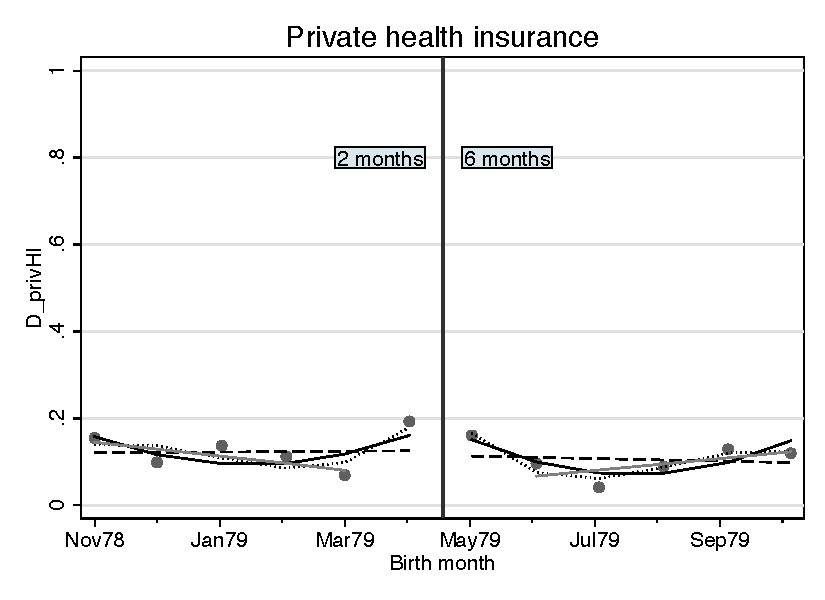
\includegraphics[width=\textwidth]{../../analysis/graphs/SOEP/D_privHI_RD.pdf}
\end{subfigure}
\quad
\begin{subfigure}[h]{0.48\textwidth}\centering
	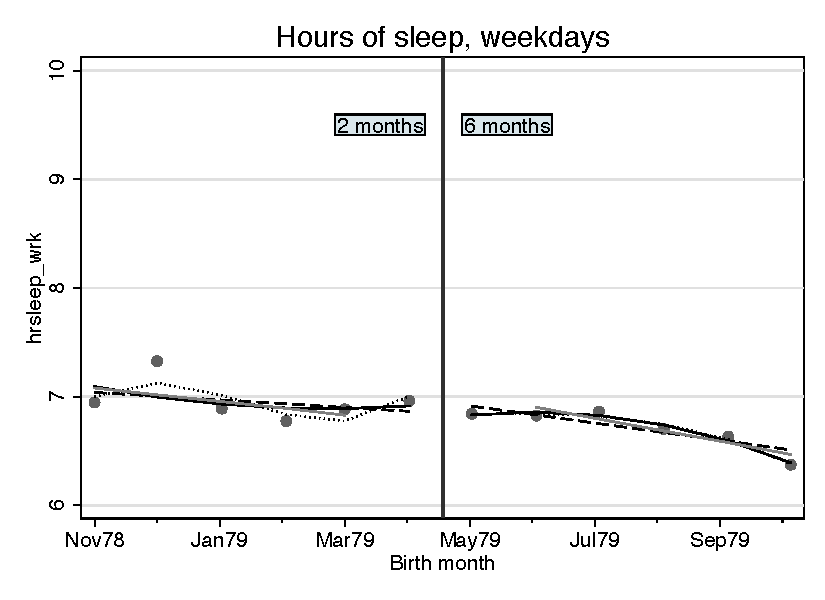
\includegraphics[width=\textwidth]{../../analysis/graphs/SOEP/hrsleep_wrk_RD.pdf}
\end{subfigure}

\begin{subfigure}[h]{0.48\textwidth}\centering
	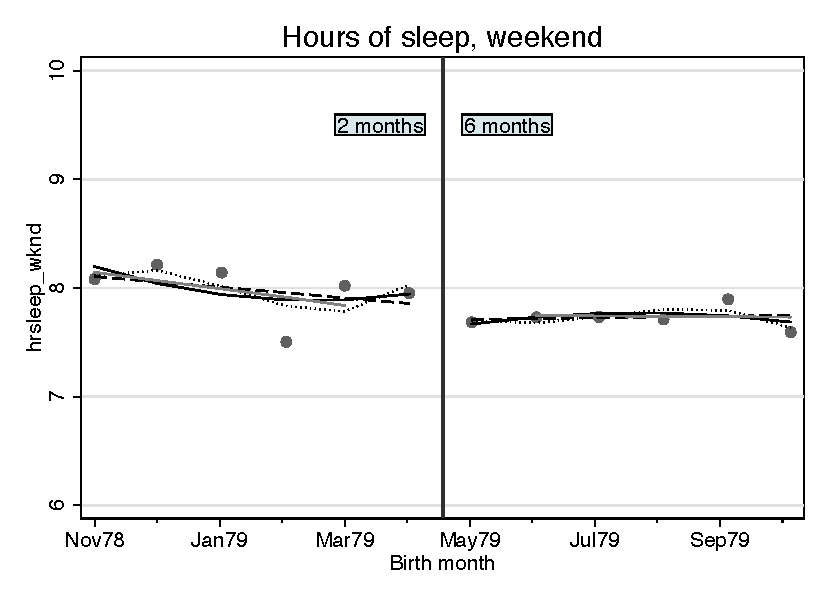
\includegraphics[width=\textwidth]{../../analysis/graphs/SOEP/hrsleep_wknd_RD.pdf}
\end{subfigure}


\caption{Impact of 1979 maternity leave expansion on Health behavior}\label{fig: RD_HB}
\begin{minipage}{\textwidth} % choose width suitably
{\footnotesize \textit{Note:} The averages correspond to one month bins. The solid vertical line divides pre- and post-reform time span, i.e. two or six months of job-protected leave after childbirth. Sample only contains individual born within half a year of the cutoff date. \newline \textit{Source: }German Socio-Economic Panel, version 31\par}
\end{minipage}
\end{figure}





\clearpage
%%%%%%%%%%%%%%%%%%%%%%%%%%%%%%%%%%%%%%%%%%%%%%%%
%		Life course graphs
%%%%%%%%%%%%%%%%%%%%%%%%%%%%%%%%%%%%%%%%%%%%%%%%
%		 BM
\newpage
\begin{figure}[p]
\begin{subfigure}[h]{0.48\textwidth}\centering
	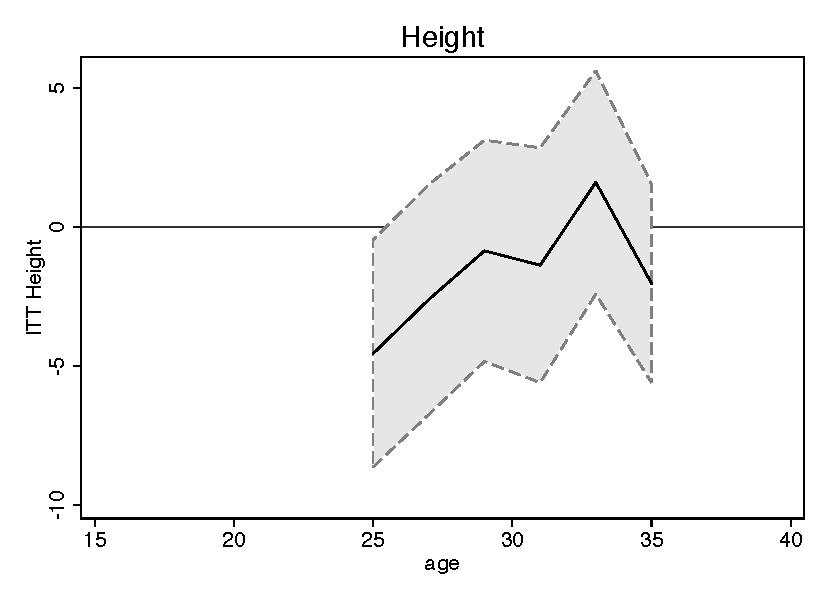
\includegraphics[width=\textwidth]{../../analysis/graphs/SOEP/Height_LC.pdf}
\end{subfigure}
\quad
\begin{subfigure}[h]{0.48\textwidth}\centering
	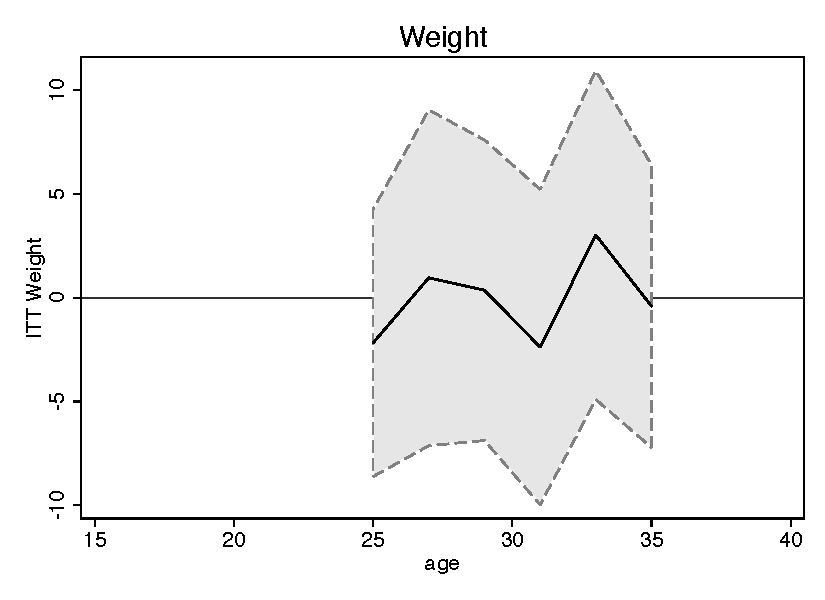
\includegraphics[width=\textwidth]{../../analysis/graphs/SOEP/Weight_LC.pdf}
\end{subfigure}

\begin{subfigure}[h]{0.48\textwidth}\centering
	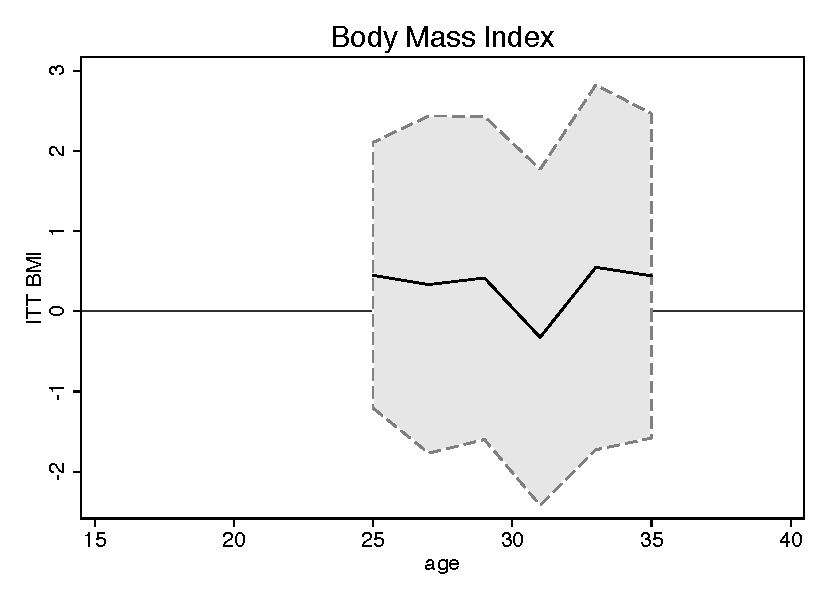
\includegraphics[width=\textwidth]{../../analysis/graphs/SOEP/BMI_LC.pdf}
\end{subfigure}
\quad
\begin{subfigure}[h]{0.48\textwidth}\centering
	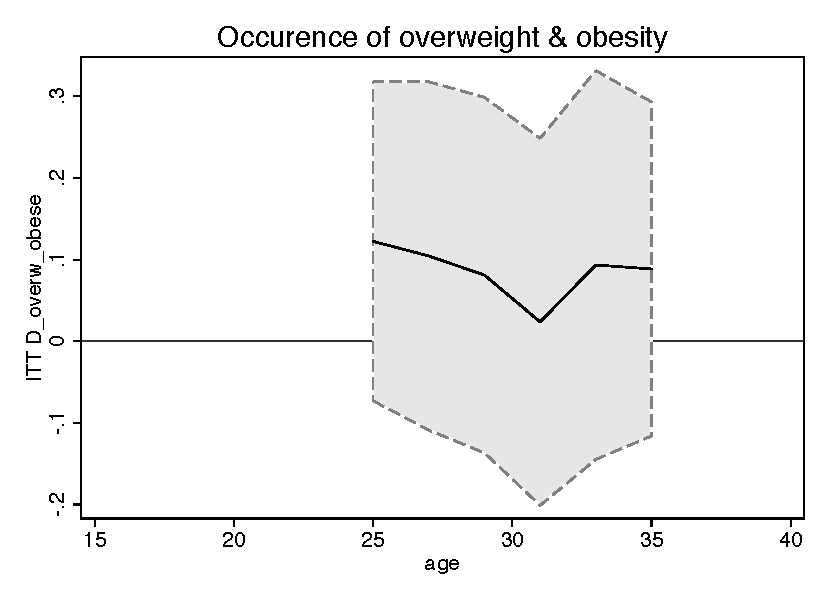
\includegraphics[width=\textwidth]{../../analysis/graphs/SOEP/D_overw_obese_LC.pdf}
\end{subfigure}
\caption{Impact of 1979 maternity leave expansion on biometric outcomes over the life-course}\label{fig: LC_BM}
\begin{minipage}{\textwidth} % choose width suitably
{\footnotesize \textit{Note:} The figures plot DD-RD estimates (along with 90\% confidence intervals) for the impact of the reform on outcomes by the age of the respondent. Estimates come from a regression based on equation \ref{eq:RD+DD}, which are run separately for each age value. Dependent on the frequency of the variable in the survey, the length of the life-course is not the same for all variables. The control group is comprised of children that are born in the same months but two years before and one year after the reform (i.e. children born between November 1976 and October 1977, November 1977 and October 1978, and November 1979 and October 1980).  \newline \textit{Source: }German Socio-Economic Panel, version 31\par}
\end{minipage}
\end{figure}
%		 OH
\newpage
\begin{figure}[p]
\begin{subfigure}[h]{0.48\textwidth}\centering
	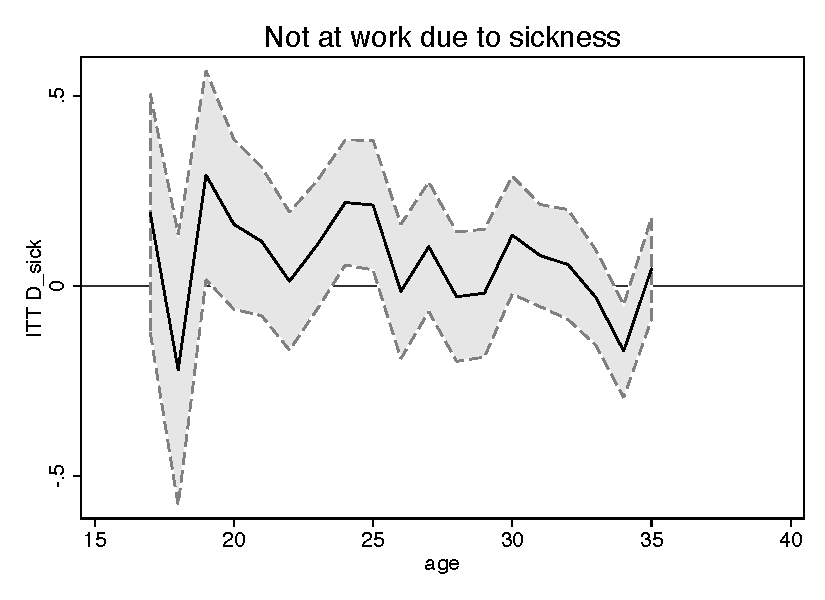
\includegraphics[width=\textwidth]{../../analysis/graphs/SOEP/D_sick_LC.pdf}
\end{subfigure}
\quad
\begin{subfigure}[h]{0.48\textwidth}\centering
	\includegraphics[width=\textwidth]{../../analysis/graphs/SOEP/Days_sick_LC.pdf}
\end{subfigure}

\begin{subfigure}[h]{0.48\textwidth}\centering
	\includegraphics[width=\textwidth]{../../analysis/graphs/SOEP/D_doctor_LC.pdf}
\end{subfigure}
\quad
\begin{subfigure}[h]{0.48\textwidth}\centering
	\includegraphics[width=\textwidth]{../../analysis/graphs/SOEP/Docvisits_LC.pdf}
\end{subfigure}



\begin{subfigure}[h]{0.48\textwidth}\centering
	\includegraphics[width=\textwidth]{../../analysis/graphs/SOEP/D_hospital_LC.pdf}
\end{subfigure}
\quad
\begin{subfigure}[h]{0.48\textwidth}\centering
	\includegraphics[width=\textwidth]{../../analysis/graphs/SOEP/D_disab_LC.pdf}
\end{subfigure}

\begin{subfigure}[h]{0.48\textwidth}\centering
	\includegraphics[width=\textwidth]{../../analysis/graphs/SOEP/D_illness_LC.pdf}
\end{subfigure}
\quad
\begin{subfigure}[h]{0.48\textwidth}\centering
	\includegraphics[width=\textwidth]{../../analysis/graphs/SOEP/D_chronill_LC.pdf}
\end{subfigure}

\caption{Impact of 1979 maternity leave expansion on objective health outcomes over the life-course}\label{fig: LC_OH}
\begin{minipage}{\textwidth} % choose width suitably
{\footnotesize \textit{Note:} The figures plot DD-RD estimates (along with 90\% confidence intervals) for the impact of the reform on outcomes by the age of the respondent. Estimates come from a regression based on equation \ref{eq:RD+DD}, which are run separately for each age value. Dependent on the frequency of the variable in the survey, the length of the life-course is not the same for all variables. The control group is comprised of children that are born in the same months but two years before and one year after the reform (i.e. children born between November 1976 and October 1977, November 1977 and October 1978, and November 1979 and October 1980).\newline \textit{Source: }German Socio-Economic Panel, version 31\par}
\end{minipage}
\end{figure}
% 		SH
\newpage
\begin{figure}[p]
\begin{subfigure}[h]{0.48\textwidth}\centering
	\includegraphics[width=\textwidth]{../../analysis/graphs/SOEP/Health_concerns_LC.pdf}
\end{subfigure}
\quad
\begin{subfigure}[h]{0.48\textwidth}\centering
	\includegraphics[width=\textwidth]{../../analysis/graphs/SOEP/SAH_5_LC.pdf}
\end{subfigure}

\begin{subfigure}[h]{0.48\textwidth}\centering
	\includegraphics[width=\textwidth]{../../analysis/graphs/SOEP/SAS_10_LC.pdf}
\end{subfigure}
\quad
\begin{subfigure}[h]{0.48\textwidth}\centering
	\includegraphics[width=\textwidth]{../../analysis/graphs/SOEP/Problems_activ_LC.pdf}
\end{subfigure}



%\begin{subfigure}[h]{0.48\textwidth}\centering
%	\includegraphics[width=\textwidth]{Handle_stress_LC.pdf}
%\end{subfigure}
%\quad
\begin{subfigure}[h]{0.48\textwidth}\centering
	\includegraphics[width=\textwidth]{../../analysis/graphs/SOEP/Phys_pain_LC.pdf}
\end{subfigure}
\quad
\begin{subfigure}[h]{0.48\textwidth}\centering
	\includegraphics[width=\textwidth]{../../analysis/graphs/SOEP/Constr_soc_contact_LC.pdf}
\end{subfigure}


\caption{Impact of 1979 maternity leave expansion on subjective health outcomes over the life-course}\label{fig: LC_SH}
\begin{minipage}{\textwidth} % choose width suitably
{\footnotesize \textit{Note:} The figures plot DD-RD estimates (along with 90\% confidence intervals) for the impact of the reform on outcomes by the age of the respondent. Estimates come from a regression based on equation \ref{eq:RD+DD}, which are run separately for each age value. Dependent on the frequency of the variable in the survey, the length of the life-course is not the same for all variables. The control group is comprised of children that are born in the same months but two years before and one year after the reform (i.e. children born between November 1976 and October 1977, November 1977 and October 1978, and November 1979 and October 1980). \newline \textit{Source: }German Socio-Economic Panel, version 31\par}
\end{minipage}
\end{figure}

%		 HB
\newpage
\begin{figure}[p]
\begin{subfigure}[h]{0.48\textwidth}\centering
	\includegraphics[width=\textwidth]{../../analysis/graphs/SOEP/Healthydiet_LC.pdf}
\end{subfigure}
\quad
\begin{subfigure}[h]{0.48\textwidth}\centering
	\includegraphics[width=\textwidth]{../../analysis/graphs/SOEP/D_smoke_LC.pdf}
\end{subfigure}

\begin{subfigure}[h]{0.48\textwidth}\centering
	\includegraphics[width=\textwidth]{../../analysis/graphs/SOEP/Cigarettes_LC.pdf}
\end{subfigure}
\quad
\begin{subfigure}[h]{0.48\textwidth}\centering
	\includegraphics[width=\textwidth]{../../analysis/graphs/SOEP/Alcohol_LC.pdf}
\end{subfigure}



\begin{subfigure}[h]{0.48\textwidth}\centering
	\includegraphics[width=\textwidth]{../../analysis/graphs/SOEP/D_privHI_LC.pdf}
\end{subfigure}
\quad
\begin{subfigure}[h]{0.48\textwidth}\centering
	\includegraphics[width=\textwidth]{../../analysis/graphs/SOEP/hrsleep_wrk_LC.pdf}
\end{subfigure}

\begin{subfigure}[h]{0.48\textwidth}\centering
	\includegraphics[width=\textwidth]{../../analysis/graphs/SOEP/hrsleep_wknd_LC.pdf}
\end{subfigure}


\caption{Impact of 1979 maternity leave expansion on Health behavior over the life-course}\label{fig: LC_HB}
\begin{minipage}{\textwidth} % choose width suitably
{\footnotesize \textit{Note:} The figures plot DD-RD estimates (along with 90\% confidence intervals) for the impact of the reform on outcomes by the age of the respondent. Estimates come from a regression based on equation \ref{eq:RD+DD}, which are run separately for each age value. Dependent on the frequency of the variable in the survey, the length of the life-course is not the same for all variables. The control group is comprised of children that are born in the same months but two years before and one year after the reform (i.e. children born between November 1976 and October 1977, November 1977 and October 1978, and November 1979 and October 1980). \newline \textit{Source: }German Socio-Economic Panel, version 31\par}
\end{minipage}
\end{figure}





    
    
    
    
    
    
    
    
    
    
    
    
    
    
    
    
    
    
    
    
    
    
    
    
    
    
\clearpage
%%%%%%%%%%%%%%%%%%%%%%%%%%%%%%%%%%%%%%%%%%%%%%%%
%		LOCATIONS
%%%%%%%%%%%%%%%%%%%%%%%%%%%%%%%%%%%%%%%%%%%%%%%%
%		 BM
\newpage
\begin{figure}[p]
\begin{subfigure}[h]{0.48\textwidth}\centering
	\includegraphics[width=\textwidth]{../../analysis/graphs/SOEP/LOCHeight.pdf}
\end{subfigure}
\quad
\begin{subfigure}[h]{0.48\textwidth}\centering
	\includegraphics[width=\textwidth]{../../analysis/graphs/SOEP/LOCWeight.pdf}
\end{subfigure}
\par\bigskip
\begin{subfigure}[h]{0.48\textwidth}\centering
	\includegraphics[width=\textwidth]{../../analysis/graphs/SOEP/LOCBMI.pdf}
\end{subfigure}
\quad
\begin{subfigure}[h]{0.48\textwidth}\centering
	\includegraphics[width=\textwidth]{../../analysis/graphs/SOEP/LOCD_overw_obese.pdf}
\end{subfigure}
\caption{Impact of 1979 maternity leave expansion on biometric outcomes, by federal state}\label{fig: LOC_BM}
\begin{minipage}{\textwidth} % choose width suitably
{\footnotesize \textit{Note:} The figures plot DD-RD estimates for the impact of the reform on health outcomes by the federal state. Estimates come from a regression based on equation \ref{eq:RD+DD}, which are run separately for each federal state. The control group is comprised of children that are born in the same months but two years before and one year after the reform (i.e. children born between November 1976 and October 1977, November 1977 and October 1978, and November 1979 and October 1980). \newline \textit{Source: }German Socio-Economic Panel, version 31\par}
\end{minipage}
\end{figure}


%
%%		 OH
%\newpage
%\begin{figure}[p]\centering
%\begin{subfigure}[h]{0.4\textwidth}\centering
%	\includegraphics[width=\textwidth]{LOCD_sick.pdf}
%\end{subfigure}
%\quad
%\begin{subfigure}[h]{0.4\textwidth}\centering
%	\includegraphics[width=\textwidth]{LOCDays_sick.pdf}
%\end{subfigure}
%\par\medskip
%\begin{subfigure}[h]{0.4\textwidth}\centering
%	\includegraphics[width=\textwidth]{LOCD_doctor.pdf}
%\end{subfigure}
%\quad
%\begin{subfigure}[h]{0.4\textwidth}\centering
%	\includegraphics[width=\textwidth]{LOCDocvisits.pdf}
%\end{subfigure}
%\par\medskip
%
%
%
%\begin{subfigure}[h]{0.4\textwidth}\centering
%	\includegraphics[width=\textwidth]{LOCD_hospital.pdf}
%\end{subfigure}
%\quad
%\begin{subfigure}[h]{0.4\textwidth}\centering
%	\includegraphics[width=\textwidth]{LOCD_disab.pdf}
%\end{subfigure}
%\par\medskip
%
%\begin{subfigure}[h]{0.4\textwidth}\centering
%	\includegraphics[width=\textwidth]{LOCD_illness.pdf}
%\end{subfigure}
%\quad
%\begin{subfigure}[h]{0.4\textwidth}\centering
%	\includegraphics[width=\textwidth]{LOCD_chronill.pdf}
%\end{subfigure}
%
%\caption{Impact of 1979 maternity leave expansion on objective health outcomes, by federal state}\label{fig: LOC_OH}
%\begin{minipage}{\textwidth} % choose width suitably
%{\footnotesize \textit{Note:} The figures plot DD-RD estimates for the impact of the reform on health outcomes by the federal state. Estimates come from a regression based on equation \ref{eq:RD+DD}, which are run separately for each federal state. The control group is comprised of children that are born in the same months but two years before and one year after the reform (i.e. children born between November 1976 and October 1977, November 1977 and October 1978, and November 1979 and October 1980). \newline \textit{Source: }German Socio-Economic Panel, version 31\par}
%\end{minipage}
%\end{figure}
%% 		SH
%\newpage
%\begin{figure}[p]\centering
%\begin{subfigure}[h]{0.4\textwidth}\centering
%	\includegraphics[width=\textwidth]{LOCHealth_concerns.pdf}
%\end{subfigure}
%\quad
%\begin{subfigure}[h]{0.4\textwidth}\centering
%	\includegraphics[width=\textwidth]{LOCSAH_5.pdf}
%\end{subfigure}
%\par\medskip
%
%\begin{subfigure}[h]{0.4\textwidth}\centering
%	\includegraphics[width=\textwidth]{LOCSAS_10.pdf}
%\end{subfigure}
%\quad
%\begin{subfigure}[h]{0.4\textwidth}\centering
%	\includegraphics[width=\textwidth]{LOCProblems_activ.pdf}
%\end{subfigure}
%
%\par\medskip
%
%
%\begin{subfigure}[h]{0.4\textwidth}\centering
%	\includegraphics[width=\textwidth]{LOCHandle_stress.pdf}
%\end{subfigure}
%\quad
%\begin{subfigure}[h]{0.4\textwidth}\centering
%	\includegraphics[width=\textwidth]{LOCPhys_pain.pdf}
%\end{subfigure}
%\par\medskip
%
%\begin{subfigure}[h]{0.4\textwidth}\centering
%	\includegraphics[width=\textwidth]{LOCConstr_soc_contact.pdf}
%\end{subfigure}
%
%
%\caption{Impact of 1979 maternity leave expansion on subjective health outcomes, by federal state}\label{fig: LOC_SH}
%\begin{minipage}{\textwidth} % choose width suitably
%{\footnotesize \textit{Note:} The figures plot DD-RD estimates for the impact of the reform on health outcomes by the federal state. Estimates come from a regression based on equation \ref{eq:RD+DD}, which are run separately for each federal state. The control group is comprised of children that are born in the same months but two years before and one year after the reform (i.e. children born between November 1976 and October 1977, November 1977 and October 1978, and November 1979 and October 1980). \newline \textit{Source: }German Socio-Economic Panel, version 31\par}
%\end{minipage}
%\end{figure}

%		 HB
\newpage
\begin{figure}[p]\centering
\begin{subfigure}[h]{0.4\textwidth}\centering
	\includegraphics[width=\textwidth]{../../analysis/graphs/SOEP/LOCHealthydiet.pdf}
\end{subfigure}
\quad
\begin{subfigure}[h]{0.4\textwidth}\centering
	\includegraphics[width=\textwidth]{../../analysis/graphs/SOEP/LOCD_smoke.pdf}
\end{subfigure}
\par\medskip
\begin{subfigure}[h]{0.4\textwidth}\centering
	\includegraphics[width=\textwidth]{../../analysis/graphs/SOEP/LOCCigarettes.pdf}
\end{subfigure}
\quad
\begin{subfigure}[h]{0.4\textwidth}\centering
	\includegraphics[width=\textwidth]{../../analysis/graphs/SOEP/LOCAlcohol.pdf}
\end{subfigure}
\par\medskip



\begin{subfigure}[h]{0.4\textwidth}\centering
	\includegraphics[width=\textwidth]{../../analysis/graphs/SOEP/LOCD_privHI.pdf}
\end{subfigure}
\quad
\begin{subfigure}[h]{0.4\textwidth}\centering
	\includegraphics[width=\textwidth]{../../analysis/graphs/SOEP/LOChrsleep_wrk.pdf}
\end{subfigure}
\par\medskip

\begin{subfigure}[h]{0.4\textwidth}\centering
	\includegraphics[width=\textwidth]{../../analysis/graphs/SOEP/LOChrsleep_wknd.pdf}
\end{subfigure}


\caption{Impact of 1979 maternity leave expansion on Health behavior, by federal state}\label{fig: LOC_HB}
\begin{minipage}{\textwidth} % choose width suitably
{\footnotesize \textit{Note:} The figures plot DD-RD estimates for the impact of the reform on health outcomes by the federal state. Estimates come from a regression based on equation \ref{eq:RD+DD}, which are run separately for each federal state. The control group is comprised of children that are born in the same months but two years before and one year after the reform (i.e. children born between November 1976 and October 1977, November 1977 and October 1978, and November 1979 and October 1980). \newline \textit{Source: }German Socio-Economic Panel, version 31\par}
\end{minipage}
\end{figure}    
    
    
    
    
    
    
    
    
    
       



%%%%%%%%%%%%%%%%%%%%%%%%%%%%%%%%%%%%%%%%%%%%%%%%
%%%%%%%%%%%%%%%%%%%%%%%%%%%%%%%%%%%%%%%%%%%%%%%%
%		ADDITIONAL TABLES
%%%%%%%%%%%%%%%%%%%%%%%%%%%%%%%%%%%%%%%%%%%%%%%%
%%%%%%%%%%%%%%%%%%%%%%%%%%%%%%%%%%%%%%%%%%%%%%%%
\clearpage
\newpage
\subsection{Tables}
\renewcommand\thetable{A\arabic{table}}
\setcounter{table}{0} 
%\captionsetup[subfigure]{labelformat=parens}


\begin{table}[p]\centering
\caption{Number of observations, per cohort}\label{tab:observations}
\begin{tabular}{lcc}
\toprule
Cohort & Number of individuals & Number of observations \\ 
\midrule
Control 1 (Nov76 - Oct77) & 570 & 3263 \\ 
Control 2 (Nov77 - Oct78) & 605 & 3610 \\
Control 3 (Nov79 - Oct80) & 612 & 3341 \\
Treatment (Nov78 - Oct79) & 627 & 3647 \\
\midrule
Total & 2414 & 13861 \\
\bottomrule
\end{tabular} 
\begin{minipage}{0.9\textwidth} % choose width suitably
{\footnotesize \textit{Note:} This table reports the number of individuals and observations for different cohorts.\newline \textit{Source: }German Socio-Economic Panel, version 31\par}
\end{minipage}
\end{table}


\clearpage

\newpage
%%%%%%%%%%%%%%%%%%%%%%%%%%%%%%%%%%%%%%%%%%%%%%%%%%%%%%
% SUMMARY STATISTICS EXTENDED, MIT UNTERSCHIED AFTER IN C&T
%%%%%%%%%%%%%%%%%%%%%%%%%%%%%%%%%%%%%%%%%%%%%%%%%%%%%%

\newgeometry{
	top    = 3.5cm,
	bottom = 1.2cm,
	left   = 2.3cm,
	right  = 2.3cm}	
	
	
		\setlength\FHoffset{-1.5cm} %hier müssten es eigentlcih 3cm sein, sieht aber scheise aus
\fancyheadoffset{\FHoffset}



\begin{landscape}
	
\begin{center}
{\renewcommand{\tabcolsep}{2pt}
\begin{longtable}{l*{17}{c}}

\caption{Summary statistics}\label{tab:SummaryStatistics}\\
\toprule
& & \multicolumn{7}{c}{Control (\(N\)=10214)} & & & \multicolumn{7}{c}{Treatment (\(N\)=3647)}\\
\cmidrule{3-9}\cmidrule{12-18}
& & \multicolumn{3}{c}{Pre} & & \multicolumn{3}{c}{Post} & & & \multicolumn{3}{c}{Pre} & & \multicolumn{3}{c}{Post}\\
\cmidrule{3-5}\cmidrule{7-9}\cmidrule{12-14}\cmidrule{16-18}

\textit{Variable} & & \textit{Range} & \textit{mean} & \textit{s.d.}& & \textit{Range} & \textit{mean} & \textit{s.d.} & & & \textit{Range} & \textit{mean} & \textit{s.d.} & &\textit{Range} & \textit{mean} & \textit{s.d.} \\
\midrule\\
\endfirsthead
\multicolumn{18}{c}
{\tablename\ \thetable\ -- \textit{Continued from previous page}} \\
\toprule
& & \multicolumn{7}{c}{Control (\(N\)=10214)} & & & \multicolumn{7}{c}{Treatment (\(N\)=3647)}\\
\cmidrule{3-9}\cmidrule{12-18}
& & \multicolumn{3}{c}{Pre} & & \multicolumn{3}{c}{Post} & & & \multicolumn{3}{c}{Pre} & & \multicolumn{3}{c}{Post}\\
\cmidrule{3-5}\cmidrule{7-9}\cmidrule{12-14}\cmidrule{16-18}

\textit{Variable} & & \textit{Range} & \textit{mean} & \textit{s.d.}& & \textit{Range} & \textit{mean} & \textit{s.d.} & & & \textit{Range} & \textit{mean} & \textit{s.d.} & &\textit{Range} & \textit{mean} & \textit{s.d.} \\
\bottomrule
\endhead
\bottomrule \multicolumn{9}{l}{\textit{Continued on next page}} \\
\endfoot
\bottomrule
\endlastfoot

\underline{A: Background Characteristics} \\
%%%%%%%%%%%%%%%%%%%%%%%%%%%%%%%%%%%%%
	% GENERAL CHARACTERISTICS
%%%%%%%%%%%%%%%%%%%%%%%%%%%%%%%%%%%%%


Sex & & \{0,1\} &0.52 &0.50 &  & \{0,1\} &0.57 &0.50 &  &  & \{0,1\} &0.56 &0.50 &  & \{0,1\} &0.54 &0.50 \\ 
Age & & [16,38] & 28.27 & 5.83 &  & [17,37] & 27.97 & 5.71 &  &  & [17,36] & 27.59 & 5.42 &  & [15,35] & 27.73  & 5.48 \\ 
D\_migback & & \{0,1\} &0.23 &0.42 &  & \{0,1\} &0.22 &0.41 &  &  & \{0,1\} &0.20 &0.40 &  & \{0,1\} &0.22 &0.42 \\ 
D\_married & & \{0,1\} &0.37 &0.48 &  & \{0,1\} &0.35 &0.48 &  &  & \{0,1\} &0.31 &0.46 &  & \{0,1\} &0.36 &0.48 \\ 
D\_child & & \{0,1\} &0.43 &0.49 &  & \{0,1\} &0.40 &0.49 &  &  & \{0,1\} &0.35 &0.48 &  & \{0,1\} &0.40 &0.49 \\ 
Numchild & & [1,7] & 1.84 &0.87 &  & [1,7] & 1.89 &0.91 &  &  & [1,4] & 1.73 &0.72 &  & [1,6] & 1.84 &0.87 \\ 
D\_siblings & & \{0,1\} &0.88 &0.32 &  & \{0,1\} &0.87 &0.34 &  &  & \{0,1\} &0.89 &0.31 &  & \{0,1\} &0.94 &0.24 \\ 
D\_employed & & \{0,1\} &0.83 &0.38 &  & \{0,1\} &0.83 &0.37 &  &  & \{0,1\} &0.84 &0.37 &  & \{0,1\} &0.79 &0.41 \\ 
HHInc & & [0,375021] & 43511 & 32328 &  & [0,581236] & 44728 & 32647 &  &  & [0,289415] & 45530 & 33759 &  & [0,310846] & 42282 & 31115 \\ 
Yrs\_schooling & & [7,18] & 12.28 & 2.88 &  & [7,18] & 12.09 & 2.67 &  &  & [7,18] & 12.58 & 2.77 &  & [7,18] & 12.56 & 2.54 \\ 
\textit{School certificate}\\
\quad \quad Track1 (Hauptschule) & & \{0,1\} &0.20 &0.40 &  & \{0,1\} &0.24 &0.43 &  &  & \{0,1\} &0.18 &0.38 &  & \{0,1\} &0.25 &0.43 \\ 
\quad \quad Track2 (Realschule) & & \{0,1\} &0.32 &0.47 &  & \{0,1\} &0.33 &0.47 &  &  & \{0,1\} &0.29 &0.45 &  & \{0,1\} &0.24 &0.43 \\ 
\quad \quad Track3 (Gymnasium) & & \{0,1\} &0.31 &0.46 &  & \{0,1\} &0.27 &0.45 &  &  & \{0,1\} &0.37 &0.48 &  & \{0,1\} &0.33 &0.47 \\ 

 



%%%%%%%%%%%%%%%%%%%%%%%%%%%%%%%%%%%%%
\\	% BIOMETRIC MEASURES
\underline{B.1: Biometric measures}\\
%%%%%%%%%%%%%%%%%%%%%%%%%%%%%%%%%%%%% 
Height & & [149,199] & 174.41 & 9.11 &  & [117,210] & 173.81 & 9.23 &  &  & [152,203] & 174.36 & 9.25 &  & [149,200] & 173.87 & 9.68 \\ 
Weight & & [40,250] & 76.21 & 17.51 &  & [43,180] & 74.41 & 17.22 &  &  & [48,195] & 76.41 & 17.55 &  & [39,200] & 75.80 & 19.46 \\ 
BMI & & [15.43,73.05] & 24.97 & 5.06 &  & [15.5,55.56] & 24.50 & 4.75 &  &  & [15.73,58.23] & 24.99 & 4.73 &  & [16.44,63.29] & 24.83 & 5.39 \\ 
D\_overw\_obese (BMI$ >$25) & & \{0,1\} &0.41 &0.49 &  & \{0,1\} &0.36 &0.48 &  &  & \{0,1\} &0.41 &0.49 &  & \{0,1\} &0.40 &0.49 \\ 




%%%%%%%%%%%%%%%%%%%%%%%%%%%%%%%%%%%%%
\\	% OBJECTIVE MEASURES
\underline{B.2: Objective measures}\\
%%%%%%%%%%%%%%%%%%%%%%%%%%%%%%%%%%%%%
D\_sick & & \{0,1\} &0.62 &0.49 &  & \{0,1\} &0.58 &0.49 &  &  & \{0,1\} &0.57 &0.49 &  & \{0,1\} &0.59 &0.49 \\ 
Days\_sick & & [1,365] & 8.22 & 20.89 &  & [1,365] & 7.42 & 19.6 &  &  & [1,365] & 7.06 & 19.61 &  & [1,365] & 8.39 & 24.25 \\ 
D\_doctor & & \{0,1\} &0.62 &0.49 &  & \{0,1\} &0.61 &0.49 &  &  & \{0,1\} &0.61 &0.49 &  & \{0,1\} &0.65 &0.48 \\ 
Docvisits & & [1,99] & 2.00 & 3.51 &  & [1,50] & 1.85 & 2.93 &  &  & [1,60] & 2.00 & 3.72 &  & [1,90] & 2.26 & 4.39 \\ 
D\_hospital & & \{0,1\} &0.11 &0.31 &  & \{0,1\} &0.10 &0.30 &  &  & \{0,1\} &0.11 &0.31 &  & \{0,1\} &0.12 &0.33 \\ 
D\_disab & & \{0,1\} &0.03 &0.18 &  & \{0,1\} &0.02 &0.14 &  &  & \{0,1\} &0.02 &0.15 &  & \{0,1\} &0.02 &0.13 \\ 
D\_illness & & \{0,1\} &0.38 &0.49 &  & \{0,1\} &0.35 &0.48 &  &  & \{0,1\} &0.32 &0.47 &  & \{0,1\} &0.36 &0.48 \\ 
D\_chronill & & \{0,1\} &0.27 &0.44 &  & \{0,1\} &0.25 &0.43 &  &  & \{0,1\} &0.23 &0.42 &  & \{0,1\} &0.28 &0.45 \\ 






%%%%%%%%%%%%%%%%%%%%%%%%%%%%%%%%%%%%%
\\	% SUBJECTIVE MEASURES
\underline{B.3: Subjective measures}\\
%%%%%%%%%%%%%%%%%%%%%%%%%%%%%%%%%%%%%
Health\_concerns & & [1,3] & 1.63 &0.67 &  & [1,3] & 1.59 &0.65 &  &  & [1,3] & 1.53 &0.64 &  & [1,3] & 1.65 &0.67 \\ 
SAH\_5 & & [1,5] & 3.81 &0.86 &  & [1,5] & 3.87 &0.85 &  &  & [1,5] & 3.91 &0.86 &  & [1,5] & 3.77 &0.90 \\ 
SAS\_10 & & [0,10] & 6.72 & 2.19 &  & [0,10] & 6.87 & 2.24 &  &  & [0,10] & 6.98 & 2.27 &  & [0,10] & 6.8 & 2.16 \\ 
Problems\_activ & & [1,3] & 1.29 &0.53 &  & [1,3] & 1.26 &0.50 &  &  & [1,3] & 1.24 &0.49 &  & [1,3] & 1.29 &0.52 \\ 
Handle\_stress & & [1,7] & 4.42 & 1.57 &  & [1,7] & 4.55 & 1.44 &  &  & [1,7] & 4.65 & 1.46 &  & [1,7] & 4.58 & 1.48 \\ 
Phys\_pain & & [1,5] & 1.78 &0.95 &  & [1,5] & 1.79 &0.95 &  &  & [1,5] & 1.66 &0.90 &  & [1,5] & 1.77 &0.98 \\ 
Constr\_soc\_contact & & [1,5] & 4.48 &0.84 &  & [1,5] & 4.44 &0.90 &  &  & [1,5] & 4.57 &0.81 &  & [1,5] & 4.40 &0.94 \\ 





%%%%%%%%%%%%%%%%%%%%%%%%%%%%%%%%%%%%%
\\	% HEALTH BEHAVIOR
\underline{B.4: Health behavior}\\
%%%%%%%%%%%%%%%%%%%%%%%%%%%%%%%%%%%%%
Healthydiet & & [1,4] & 2.41 &0.73 &  & [1,4] & 2.44 &0.73 &  &  & [1,4] & 2.49 &0.75 &  & [1,4] & 2.42 &0.72 \\ 
D\_smoke & & \{0,1\} &0.39 &0.49 &  & \{0,1\} &0.39 &0.49 &  &  & \{0,1\} &0.34 &0.48 &  & \{0,1\} &0.43 &0.50 \\ 
Cigarettes & & [1,60] & 15.24 & 8.65 &  & [1,50] & 14.01 & 7.20 &  &  & [1,30] & 12.93 & 6.69 &  & [1,40] & 13.96 & 7.15 \\ 
Alcohol & & [1,4] & 2.63 &0.90 &  & [1,4] & 2.51 &0.85 &  &  & [1,4] & 2.68 &0.79 &  & [1,4] & 2.49 & 1.00 \\ 
D\_privHI & & \{0,1\} &0.09 &0.29 &  & \{0,1\} &0.08 &0.28 &  &  & \{0,1\} &0.12 &0.33 &  & \{0,1\} &0.11 &0.31 \\ 
Hrsleep\_wrk & & [2,12] & 6.80 & 1.09 &  & [3,12] & 6.82 & 1.09 &  &  & [2,10] & 6.95 & 1.01 &  & [3,10] & 6.73 & 1.05 \\ 
Hrsleep\_wknd & & [1,12] & 7.77 & 1.35 &  & [3,14] & 7.84 & 1.36 &  &  & [4,20] & 7.97 & 1.41 &  & [3,20] & 7.73 & 1.37 
%%%%%%%%%%%%%%%%%%%%%%%%%%%%%%%%%%%%%
\end{longtable}}
\end{center}
\vspace{-1cm}\hspace{1.5cm}
\begin{minipage}{1.35\textwidth} % choose width suitably
{\footnotesize \textit{Note:} This table reports summary statistics for treatment and control group separately. Panel A presents individual background characteristics, panel B1 biometric indicators, panel B2 shows objective - and panel B3 subjective health measures. Panel B4 covers health behavior. The sample contains outcomes over the period 1993-2014.\newline \textit{Source: }German Socio-Economic Panel, version 31\par}
\end{minipage}

\end{landscape}
\restoregeometry




%%%%%%%%%%%%%%%%%%%%%%%%%%%%%%%%%%%%%%%%%%%%%%%%%%%%%%
%	REGRESSION DISCONTINUITY TABLES
%%%%%%%%%%%%%%%%%%%%%%%%%%%%%%%%%%%%%%%%%%%%%%%%%%%%%%
%%%%%%%
% BIOMETRIC - RD
\newgeometry{
	top    = 3.5cm,
	bottom = 1.2cm,
	left   = 2.8cm,
	right  = 2.8cm}	
	

		\setlength\FHoffset{-0.5cm} 
		\fancyheadoffset{\FHoffset}


\bigskip \bigskip

\begin{table}[p] \centering
\def\sym#1{\ifmmode^{#1}\else\(^{#1}\)\fi}
\caption{Regression Discontinuity Analysis for Biometric Outcomes}\label{tab:RD_BM}
\begin{tabular}{l*{10}{c}}
\toprule
  &\multicolumn{1}{c}{(1)}&\multicolumn{1}{c}{(2)}&\multicolumn{1}{c}{(3)}&\multicolumn{1}{c}{(4)} \\ 
\midrule\\
	             &\multicolumn{1}{c}{Height}&\multicolumn{1}{c}{Weight}&\multicolumn{1}{c}{BMI}&\multicolumn{1}{c}{D\_overw\_obese}\\
\midrule
Linear      &      -2.076         &      -2.948         &      -0.717         &      -0.116         \\
            &     (2.679)         &     (4.371)         &     (1.159)         &     (0.108)         \\
Quadratic   &      -3.562         &      -11.79         &      -3.050         &      -0.335\sym{*}  \\
            &     (5.086)         &     (8.199)         &     (2.116)         &     (0.203)         \\
Cubic       &      -12.29         &      -8.115         &     0.00395         &      -0.174         \\
            &     (10.09)         &     (16.09)         &     (4.320)         &     (0.415)         \\
Donut       &      -0.159         &       1.686         &       0.282         &     -0.0294         \\
            &     (3.885)         &     (6.839)         &     (1.851)         &     (0.162)         \\

 \bottomrule
\end{tabular}
\begin{minipage}{0.6\textwidth} % choose width suitably
{\footnotesize \textit{Note:} This table reports for different functional forms of $f(\cdot)$ RD estimates of the impact of the expansion in maternity leave from two to six months on different biometric health outcomes over the period 1993-2014. The estimates are based on equation \ref{eq:RD}. \newline
Clustered standard errors are reported in parentheses. Significance levels:+ \(p<0.15\), * \(p<0.10\), ** \(p<0.05\), *** \(p<0.01\). \newline \textit{Source: }German Socio-Economic Panel, version 31\par}
\end{minipage}
\end{table}
%%%%%%%
% OBJECTIVE HEALTH
\bigskip \bigskip \bigskip
\begin{table}[p] \centering
\def\sym#1{\ifmmode^{#1}\else\(^{#1}\)\fi}
\caption{Regression Discontinuity Analysis for Objective Health Outcomes}\label{tab:RD_OH}
\scalebox{0.9}{
\begin{tabular}{l*{10}{c}}
\toprule
 &\multicolumn{1}{c}{(1)}&\multicolumn{1}{c}{(2)}&\multicolumn{1}{c}{(3)}&\multicolumn{1}{c}{(4)}&\multicolumn{1}{c}{(5)}&\multicolumn{1}{c}{(6)}&\multicolumn{1}{c}{(7)}&\multicolumn{1}{c}{(8)} \\

\midrule\\
	             &\multicolumn{1}{c}{D\_sick}&\multicolumn{1}{c}{Days\_sick}&\multicolumn{1}{c}{D\_doctor}&\multicolumn{1}{c}{Docvisits}&\multicolumn{1}{c}{D\_hospital}&\multicolumn{1}{c}{D\_disab}&\multicolumn{1}{c}{D\_illness}&\multicolumn{1}{c}{D\_chronill}\\
\midrule
Linear      &     -0.0321         &      -0.829         &      0.0232         &       0.327         &    -0.00987         &     0.00609         &    -0.00293         &     0.00502         \\
            &    (0.0730)         &     (2.863)         &    (0.0569)         &     (0.550)         &    (0.0334)         &    (0.0227)         &     (0.134)         &    (0.0813)         \\
Quadratic   &       0.127         &       6.345         &       0.294\sym{***}&       2.529\sym{**} &     -0.0390         &     -0.0416         &       0.290         &       0.207         \\
            &     (0.146)         &     (5.561)         &     (0.105)         &     (1.137)         &    (0.0694)         &    (0.0326)         &     (0.251)         &     (0.145)         \\
Cubic       &      0.0717         &       19.38\sym{*}  &       0.303         &       4.965\sym{**} &      0.0828         &      0.0104         &       0.537         &       0.210         \\
            &     (0.283)         &     (10.29)         &     (0.216)         &     (2.115)         &     (0.136)         &    (0.0817)         &     (0.517)         &     (0.310)         \\
Donut       &     -0.0663         &      -7.137\sym{**} &     -0.0933         &      -1.038\sym{*}  &     -0.0160         &      0.0136         &      -0.189         &      -0.103         \\
            &    (0.0941)         &     (3.386)         &    (0.0855)         &     (0.535)         &    (0.0411)         &    (0.0434)         &     (0.201)         &     (0.131)         \\

 \bottomrule
\end{tabular}
}
\begin{minipage}{0.95\textwidth} % choose width suitably
{\footnotesize \textit{Note:} This table reports for different functional forms of $f(\cdot)$ RD estimates of the impact of the expansion in maternity leave from two to six months on different objective health outcomes over the period 1993-2014. The estimates are based on equation \ref{eq:RD}.\newline
Clustered standard errors are reported in parentheses. Significance levels:+ \(p<0.15\), * \(p<0.10\), ** \(p<0.05\), *** \(p<0.01\). \newline \textit{Source: }German Socio-Economic Panel, version 31\par}
\end{minipage}
\end{table}

%%%%%%%
% SUBJECTIVE HEALTh
\clearpage
\begin{table}[p] \centering
\def\sym#1{\ifmmode^{#1}\else\(^{#1}\)\fi}
\caption{Regression Discontinuity Analsis for Subjective Health Outcomes}\label{tab:RD_SH}
{\renewcommand{\tabcolsep}{2pt}
\begin{tabular}{l*{10}{c}}
\toprule
 &\multicolumn{1}{c}{(1)}&\multicolumn{1}{c}{(2)}&\multicolumn{1}{c}{(3)}&\multicolumn{1}{c}{(4)}&\multicolumn{1}{c}{(5)} &\multicolumn{1}{c}{(6)}&\multicolumn{1}{c}{(7)}\\

\midrule\\
	             &\multicolumn{1}{c}{Health\_concerns}&\multicolumn{1}{c}{SAH\_5}&\multicolumn{1}{c}{SAS\_10}&\multicolumn{1}{c}{Problems\_activ}&\multicolumn{1}{c}{Handle\_stress}&\multicolumn{1}{c}{Phys\_pain}&\multicolumn{1}{c}{Constr\_soc}\\
\midrule
Linear      &      0.0456         &      -0.110         &     -0.0651         &     -0.0795         &      0.0515         &     -0.0479         &      0.0371         \\
            &     (0.106)         &     (0.130)         &     (0.376)         &    (0.0841)         &     (0.367)         &     (0.187)         &     (0.133)         \\
Quadratic   &      0.0951         &      -0.377\sym{+}  &      -0.359         &     -0.0340         &      -1.391\sym{*}  &      -0.193         &       0.288         \\
            &     (0.206)         &     (0.245)         &     (0.693)         &     (0.171)         &     (0.710)         &     (0.385)         &     (0.252)         \\
Cubic       &       0.104         &      -0.263         &      -0.374         &      -0.520\sym{+}  &      -1.577         &      -0.542         &     -0.0913         \\
            &     (0.413)         &     (0.497)         &     (1.462)         &     (0.330)         &     (1.411)         &     (0.740)         &     (0.521)         \\
Donut       &      0.0629         &     -0.0450         &     -0.0348         &     -0.0267         &       0.857\sym{+}  &      0.0852         &     0.00455         \\
            &     (0.146)         &     (0.191)         &     (0.598)         &     (0.121)         &     (0.555)         &     (0.239)         &     (0.219)         \\

 \bottomrule
\end{tabular}}

\begin{minipage}{0.95\textwidth} % choose width suitably
{\footnotesize \textit{Note:} This table reports for different functional forms of $f(\cdot)$ RD estimates of the impact of the expansion in maternity leave from two to six months on different subjective health outcomes over the period 1993-2014. The estimates are based on equation \ref{eq:RD}.\newline
Clustered standard errors are reported in parentheses. Significance levels:+ \(p<0.15\), * \(p<0.10\), ** \(p<0.05\), *** \(p<0.01\). \newline \textit{Source: }German Socio-Economic Panel, version 31\par}
\end{minipage}
\end{table}

%%%%%%%
%  HEALTH BEHAVOR
\begin{table}[p] \centering
\def\sym#1{\ifmmode^{#1}\else\(^{#1}\)\fi}
\caption{Regression Discontinuity Analysis for Health Behavior}\label{tab:RD_HB}
\begin{tabular}{l*{10}{c}}
\toprule
 &\multicolumn{1}{c}{(1)}&\multicolumn{1}{c}{(2)}&\multicolumn{1}{c}{(3)}&\multicolumn{1}{c}{(4)}&\multicolumn{1}{c}{(5)}&\multicolumn{1}{c}{(6)}&\multicolumn{1}{c}{(7)}\\

\midrule\\
	             &\multicolumn{1}{c}{Healthydiet}&\multicolumn{1}{c}{D\_smoke}&\multicolumn{1}{c}{Cigarettes}&\multicolumn{1}{c}{Alcohol}&\multicolumn{1}{c}{D\_privHI}&\multicolumn{1}{c}{hrsleep\_wrk}&\multicolumn{1}{c}{hrsleep\_wknd}\\
\midrule
Linear      &     -0.0822         &      0.0652         &      -0.261         &       0.131         &    -0.00999         &       0.163         &      -0.103         \\
            &     (0.154)         &     (0.106)         &     (2.311)         &     (0.285)         &    (0.0617)         &     (0.180)         &     (0.235)         \\
Quadratic   &       0.121         &       0.256         &       1.030         &       0.161         &     0.00206         &      -0.222         &      -0.476         \\
            &     (0.296)         &     (0.200)         &     (4.788)         &     (0.572)         &     (0.131)         &     (0.336)         &     (0.480)         \\
Cubic       &       0.635         &       0.704\sym{*}  &      -1.081         &       0.115         &     0.00725         &      -0.879         &      -0.842         \\
            &     (0.595)         &     (0.407)         &     (8.997)         &     (1.100)         &     (0.244)         &     (0.697)         &     (0.919)         \\
Donut       &      -0.291         &     -0.0860         &      -2.515         &      0.0844         &    -0.00903         &       0.415\sym{+}  &      0.0688         \\
            &     (0.238)         &     (0.156)         &     (2.749)         &     (0.349)         &    (0.0620)         &     (0.275)         &     (0.312)         \\

 \bottomrule
\end{tabular}
\begin{minipage}{0.95\textwidth} % choose width suitably
{\footnotesize \textit{Note:} This table reports for different functional forms of $f(\cdot)$ RD estimates of the impact of the expansion in maternity leave from two to six months on different health behavior outcomes over the period 1993-2014. The estimates are based on equation \ref{eq:RD}.\newline
Clustered standard errors are reported in parentheses. Significance levels:+ \(p<0.15\), * \(p<0.10\), ** \(p<0.05\), *** \(p<0.01\). \newline \textit{Source: }German Socio-Economic Panel, version 31\par}
\end{minipage}
\end{table}




%%%%%%%%%%%%%%%%%%%%%%%%%%%%%%%%%%%%%%%%%%%%%%%%%%%%%%
%	Heterogeneity TABLES DD-RD
%%%%%%%%%%%%%%%%%%%%%%%%%%%%%%%%%%%%%%%%%%%%%%%%%%%%%%
\newgeometry{
	top    = 3.5cm,
	bottom = 1.2cm,
	left   = 3.8cm,
	right  = 3.8cm}
	
	\setlength\FHoffset{0cm} 
		\fancyheadoffset{\FHoffset}

%	HETEROGENEITY FOR BIOMETRIC OUTCOMES
\newpage
\begin{table}[htp] \centering
\def\sym#1{\ifmmode^{#1}\else\(^{#1}\)\fi}
\caption{Heterogenity Analysis for Biometric Outcomes, DD-RD Estimates}\label{tab:Heterog_BM}
\begin{tabular}{l*{10}{c}}
\toprule
&  &\multicolumn{1}{c}{(1)}&\multicolumn{1}{c}{(2)}&\multicolumn{1}{c}{(3)}&\multicolumn{1}{c}{(4)} \\ 
\midrule\\
	 &            											&\multicolumn{1}{c}{Height}&\multicolumn{1}{c}{Weight}&\multicolumn{1}{c}{BMI}&\multicolumn{1}{c}{D\_overw\_obese}\\					
\midrule & \multirow{2}{*}{\textit{Total}} 							&       0.159         &       1.192         &       0.306         &      0.0391         \\
&            											&     (1.261)         &     (2.354)         &     (0.636)         &    (0.0581)         \\
\midrule \multirow{4}{*}{\textit{Gender}} & \multirow{2}{*}{Male}        			&       0.220         &      -1.493         &      -0.523         &      0.0278         \\
&            											&     (1.360)         &     (3.292)         &     (0.921)         &    (0.0846)         \\
& \multirow{2}{*}{Female}									&      -2.049\sym{*}  &       0.839         &       0.777         &      0.0181         \\
&            											&     (1.210)         &     (2.548)         &     (0.855)         &    (0.0780)         \\
\midrule \multirow{4}{*}{\textit{Migration background}} & \multirow{2}{*}{No}			&       0.967         &       0.956         &      0.0208         &      0.0257         \\
&            											&     (1.422)         &     (2.610)         &     (0.696)         &    (0.0645)         \\
& \multirow{2}{*}{Yes}										&      -2.571         &       1.401         &       0.928         &      0.0579         \\
&            											&     (2.406)         &     (4.851)         &     (1.333)         &     (0.127)         \\
\midrule \multirow{4}{*}{\textit{Married}} & \multirow{2}{*}{No}				&      0.0440         &       2.382         &       0.769         &       0.112\sym{*}  \\
&            											&     (1.478)         &     (2.672)         &     (0.728)         &    (0.0666)         \\
& \multirow{2}{*}{Yes}										&       0.939         &      -0.634         &      -0.578         &      -0.102         \\
&            											&     (1.811)         &     (3.565)         &     (0.946)         &    (0.0822)         \\
\midrule \multirow{4}{*}{\textit{Children}} & \multirow{2}{*}{No}				&      -0.681         &      -0.533         &      0.0665         &      0.0674         \\
&            											&     (1.569)         &     (2.822)         &     (0.760)         &    (0.0717)         \\
& \multirow{2}{*}{Yes}										&       2.820\sym{*}  &       4.882         &       0.603         &     -0.0267         \\
&            											&     (1.668)         &     (3.719)         &     (1.001)         &    (0.0864)         \\
\midrule \multirow{4}{*}{\textit{Median HH Income}} & \multirow{2}{*}{Below}			&      -0.334         &       1.032         &       0.292         &      0.0467         \\
&            											&     (1.771)         &     (3.208)         &     (0.889)         &    (0.0813)         \\
& \multirow{2}{*}{Above}									&       0.602         &       1.172         &       0.239         &      0.0383         \\
&            											&     (1.811)         &     (3.331)         &     (0.861)         &    (0.0795)         \\
\midrule \multirow{6}{*}{\textit{School Certificate (Child)}} & \multirow{2}{*}{Track 1}	&      -0.980         &      -7.201         &      -2.070         &      -0.153         \\
&            											&     (2.863)         &     (5.013)         &     (1.481)         &     (0.124)         \\
& \multirow{2}{*}{Track 2}									&      -1.702         &       10.75\sym{**} &       3.672\sym{***}&       0.278\sym{**} \\
&            											&     (2.211)         &     (4.915)         &     (1.299)         &     (0.115)         \\
& \multirow{2}{*}{Track 3}									&       3.548\sym{*}  &       4.097         &       0.327         &      0.0557         \\
&            											&     (1.985)         &     (3.177)         &     (0.776)         &    (0.0876)         \\
\midrule \multirow{6}{*}{\textit{School Certificate (Par.)}} & \multirow{2}{*}{Track 1}		&      -2.287         &      -0.628         &       0.467         &      0.0392         \\
&            											&     (2.204)         &     (4.469)         &     (1.292)         &     (0.101)         \\
& \multirow{2}{*}{Track 2}									&       4.834\sym{*}  &       2.484         &      -0.537         &     -0.0416         \\
&            											&     (2.492)         &     (4.431)         &     (1.089)         &     (0.112)         \\
& \multirow{2}{*}{Track 3}									&       2.165         &       1.908         &      -0.106         &      0.0816         \\
&            											&     (3.106)         &     (4.882)         &     (1.086)         &     (0.126)         \\




 \bottomrule
\end{tabular}
\begin{minipage}{\textwidth} % choose width suitably
{\footnotesize \textit{Note:} This table reports for various subgroups DD-RD estimates of the impact of the expansion in maternity leave from two to six months on different biometric health outcomes over the period from 1993-2014. The estimates are based on equation \ref{eq:RD+DD}. The control group is comprised of children that are born in the same months but two years before and one year after the reform (i.e. children born between November 1976 and October 1977, November 1977 and October 1978, and November 1979 and October 1980).\newline
Clustered standard errors are reported in parentheses. Significance levels:+ \(p<0.15\), * \(p<0.10\), ** \(p<0.05\), *** \(p<0.01\). \newline \textit{Source: }German Socio-Economic Panel, version 31\par}
\end{minipage}
\end{table}


%	HETEROGENEITY FOR OBJECTIVE HEALTH MEASURES
\newgeometry{
	top    = 4cm,
	bottom = 4cm,
	left   = 1.25cm,
	right  = 1.25cm}	
	
	\setlength\FHoffset{-2.5cm} 
		\fancyheadoffset{\FHoffset}
\newpage
\begin{table}[htp] \centering
\def\sym#1{\ifmmode^{#1}\else\(^{#1}\)\fi}
\caption{Heterogenity Analysis for Objective Health Outcomes, DD-RD Estimates}\label{tab:Heterog_OH}
\scalebox{0.9}{
\begin{tabular}{l*{10}{c}}
\toprule
&  &\multicolumn{1}{c}{(1)}&\multicolumn{1}{c}{(2)}&\multicolumn{1}{c}{(3)}&\multicolumn{1}{c}{(4)}&\multicolumn{1}{c}{(5)}&\multicolumn{1}{c}{(6)}&\multicolumn{1}{c}{(7)}&\multicolumn{1}{c}{(8)} \\

\midrule\\
	 &            											&\multicolumn{1}{c}{D\_sick}&\multicolumn{1}{c}{Days\_sick}&\multicolumn{1}{c}{D\_doctor}&\multicolumn{1}{c}{Docvisits}&\multicolumn{1}{c}{D\_hospital}&\multicolumn{1}{c}{D\_disab}&\multicolumn{1}{c}{D\_illness}&\multicolumn{1}{c}{D\_chronill}\\
\midrule & \multirow{2}{*}{\textit{Total}} 							&      0.0506         &       2.259\sym{*}  &      0.0437         &       0.432\sym{*}  &      0.0213         &     0.00941         &      0.0771         &      0.0655\sym{+}  \\
&            											&    (0.0366)         &     (1.271)         &    (0.0308)         &     (0.236)         &    (0.0164)         &    (0.0139)         &    (0.0687)         &    (0.0442)         \\
\midrule \multirow{4}{*}{\textit{Gender}} & \multirow{2}{*}{Male}        			&      0.0980\sym{*}  &       3.440\sym{*}  &       0.104\sym{**} &       0.916\sym{***}&      0.0172         &      0.0179         &     -0.0163         &       0.107\sym{+}  \\
&            											&    (0.0511)         &     (1.896)         &    (0.0454)         &     (0.353)         &    (0.0168)         &    (0.0249)         &    (0.0992)         &    (0.0698)         \\
& \multirow{2}{*}{Female}									&     0.00383         &       1.122         &      0.0219         &       0.176         &      0.0358         &    -0.00590         &       0.166\sym{*}  &      0.0486         \\
&            											&    (0.0505)         &     (1.727)         &    (0.0357)         &     (0.314)         &    (0.0259)         &    (0.0133)         &    (0.0961)         &    (0.0569)         \\
\midrule \multirow{4}{*}{\textit{Migration background}} & \multirow{2}{*}{No}			&      0.0442         &       2.642\sym{*}  &      0.0422         &       0.396\sym{+}  &      0.0132         &      0.0120         &      0.0659         &      0.0475         \\
&            											&    (0.0420)         &     (1.479)         &    (0.0341)         &     (0.269)         &    (0.0185)         &    (0.0173)         &    (0.0761)         &    (0.0486)         \\
& \multirow{2}{*}{Yes}										&      0.0654         &       0.192         &      0.0410         &       0.584         &      0.0471         &     0.00120         &       0.207         &       0.116         \\
&            											&    (0.0768)         &     (2.497)         &    (0.0703)         &     (0.479)         &    (0.0348)         &    (0.0133)         &     (0.168)         &     (0.111)         \\
\midrule \multirow{4}{*}{\textit{Married}} & \multirow{2}{*}{No}				&      0.0397         &       0.452         &      0.0648\sym{*}  &       0.406\sym{+}  &      0.0186         &      0.0207         &       0.110         &      0.0559         \\
&            											&    (0.0465)         &     (1.482)         &    (0.0387)         &     (0.265)         &    (0.0164)         &    (0.0185)         &    (0.0906)         &    (0.0725)         \\
& \multirow{2}{*}{Yes}										&      0.0537         &       5.018\sym{**} &    -0.00650         &       0.432         &     0.00867         &     -0.0109         &      0.0444         &      0.0849\sym{+}  \\
&            											&    (0.0513)         &     (2.135)         &    (0.0435)         &     (0.414)         &    (0.0300)         &    (0.0150)         &    (0.0955)         &    (0.0540)         \\
\midrule \multirow{4}{*}{\textit{Children}} & \multirow{2}{*}{No}				&      0.0714\sym{+}  &       1.501         &      0.0524         &       0.442\sym{*}  &      0.0296\sym{*}  &      0.0232         &       0.151\sym{*}  &       0.207\sym{**} \\
&            											&    (0.0480)         &     (1.146)         &    (0.0410)         &     (0.235)         &    (0.0152)         &    (0.0201)         &    (0.0890)         &    (0.0849)         \\
& \multirow{2}{*}{Yes}										&     0.00834         &       2.169         &      0.0128         &       0.268         &     -0.0171         &    -0.00854         &     -0.0119         &      0.0172         \\
&            											&    (0.0500)         &     (2.529)         &    (0.0392)         &     (0.445)         &    (0.0293)         &    (0.0146)         &    (0.0991)         &    (0.0513)         \\
\midrule \multirow{4}{*}{\textit{Median HH Income}} & \multirow{2}{*}{Below}			&     0.00975         &       1.343         &      0.0760\sym{*}  &       0.774\sym{**} &      0.0224         &    -0.00637         &      0.0302         &     -0.0163         \\
&            											&    (0.0493)         &     (2.182)         &    (0.0440)         &     (0.394)         &    (0.0262)         &    (0.0219)         &     (0.107)         &    (0.0695)         \\
& \multirow{2}{*}{Above}									&      0.0760\sym{+}  &       2.291\sym{+}  &     0.00234         &     -0.0634         &      0.0201         &      0.0208         &      0.0578         &       0.125\sym{**} \\
&            											&    (0.0525)         &     (1.394)         &    (0.0422)         &     (0.237)         &    (0.0209)         &    (0.0181)         &    (0.0883)         &    (0.0577)         \\
\midrule \multirow{6}{*}{\textit{School Certificate (Child)}} & \multirow{2}{*}{Track 1}	&       0.105\sym{+}  &       5.477\sym{*}  &      0.0988\sym{+}  &       0.409         &      0.0228         &    -0.00629         &      -0.186         &     -0.0538         \\
&            											&    (0.0720)         &     (3.028)         &    (0.0639)         &     (0.481)         &    (0.0369)         &    (0.0462)         &     (0.147)         &    (0.0984)         \\
& \multirow{2}{*}{Track 2}									&      0.0998\sym{+}  &       2.690         &    -0.00147         &       0.246         &      0.0569\sym{*}  &    -0.00284         &       0.289\sym{*}  &      0.0427         \\
&            											&    (0.0680)         &     (3.155)         &    (0.0542)         &     (0.650)         &    (0.0305)         &    (0.0153)         &     (0.148)         &    (0.0816)         \\
& \multirow{2}{*}{Track 3}									&      0.0369         &       2.048         &      0.0467         &       0.527\sym{+}  &      0.0106         &     0.00731         &      0.0822         &       0.143\sym{*}  \\
&            											&    (0.0626)         &     (1.660)         &    (0.0533)         &     (0.333)         &    (0.0250)         &    (0.0152)         &     (0.105)         &    (0.0748)         \\
\midrule \multirow{6}{*}{\textit{School Certificate (Par.)}} & \multirow{2}{*}{Track 1}		&       0.148\sym{**} &       4.449\sym{**} &      0.0658         &       0.810\sym{**} &      0.0127         &     0.00117         &       0.145         &      0.0661         \\
&            											&    (0.0593)         &     (1.962)         &    (0.0563)         &     (0.369)         &    (0.0318)         &    (0.0276)         &     (0.113)         &    (0.0956)         \\
& \multirow{2}{*}{Track 2}									&      0.0146         &      -1.514         &      0.0946         &       0.217         &    -0.00390         &      0.0212         &     -0.0406         &       0.118         \\
&            											&    (0.0901)         &     (2.264)         &    (0.0691)         &     (0.391)         &    (0.0277)         &    (0.0352)         &     (0.129)         &     (0.115)         \\
& \multirow{2}{*}{Track 3}									&      0.0593         &       2.085         &     0.00150         &      0.0747         &     -0.0205         &      0.0111         &       0.113         &      0.0982         \\
&            											&    (0.0976)         &     (2.202)         &    (0.0766)         &     (0.456)         &    (0.0358)         &    (0.0254)         &     (0.129)         &     (0.136)         \\

 \bottomrule
\end{tabular}
}
\begin{minipage}{0.98\textwidth} % choose width suitably
{\footnotesize \textit{Note:} This table reports for various subgroups DD-RD estimates of the impact of the expansion in maternity leave from two to six months on different objective health outcomes over the period from 1993-2014. The estimates are based on equation \ref{eq:RD+DD}. The control group is comprised of children that are born in the same months but two years before and one year after the reform (i.e. children born between November 1976 and October 1977, November 1977 and October 1978, and November 1979 and October 1980).\newline
Clustered standard errors are reported in parentheses. Significance levels:+ \(p<0.15\), * \(p<0.10\), ** \(p<0.05\), *** \(p<0.01\). \newline \textit{Source: }German Socio-Economic Panel, version 31\par}
\end{minipage}
\end{table}
\restoregeometry

%	HETEROGENEITY FOR SUBJECTIVE HEALTH MEASURES
\newpage
\newgeometry{
	top    = 4cm,
	bottom = 4cm,
	left   = 1.25cm,
	right  = 1.25cm}	
\setlength\FHoffset{-2.5cm} 
		\fancyheadoffset{\FHoffset}

\begin{table}[p] \centering
\def\sym#1{\ifmmode^{#1}\else\(^{#1}\)\fi}
\caption{Heterogenity Analysis for Subjective Health Outcomes, DD-RD Estimates}\label{tab:Heterog_SH}
\scalebox{0.8}{
\begin{tabular}{l*{10}{c}}
\toprule
& &\multicolumn{1}{c}{(1)}&\multicolumn{1}{c}{(2)}&\multicolumn{1}{c}{(3)}&\multicolumn{1}{c}{(4)}&\multicolumn{1}{c}{(5)} &\multicolumn{1}{c}{(6)}&\multicolumn{1}{c}{(7)}\\

\midrule\\
	 &            											&\multicolumn{1}{c}{Health\_concerns}&\multicolumn{1}{c}{SAH\_5}&\multicolumn{1}{c}{SAS\_10}&\multicolumn{1}{c}{Problems\_activ}&\multicolumn{1}{c}{Handle\_stress}&\multicolumn{1}{c}{Phys\_pain}&\multicolumn{1}{c}{Constr\_soc\_contact}\\
\midrule & \multirow{2}{*}{\textit{Total}} 							&       0.162\sym{***}&      -0.208\sym{***}&      -0.339\sym{+}  &      0.0895\sym{*}  &      -0.178         &       0.111         &       0.140\sym{*}  \\
&            											&    (0.0547)         &    (0.0662)         &     (0.211)         &    (0.0467)         &     (0.205)         &    (0.0885)         &    (0.0780)         \\
\midrule \multirow{4}{*}{\textit{Gender}} & \multirow{2}{*}{Male}        			&       0.153\sym{**} &      -0.341\sym{***}&      -0.504\sym{+}  &      0.0936         &    -0.00810         &      0.0843         &       0.193\sym{**} \\
&            											&    (0.0766)         &    (0.0951)         &     (0.311)         &    (0.0674)         &     (0.282)         &     (0.120)         &    (0.0980)         \\
& \multirow{2}{*}{Female}									&       0.169\sym{**} &     -0.0990         &      -0.235         &      0.0974\sym{+}  &      -0.289         &       0.150         &      0.0991         \\
&            											&    (0.0773)         &    (0.0903)         &     (0.284)         &    (0.0646)         &     (0.281)         &     (0.129)         &     (0.117)         \\
\midrule \multirow{4}{*}{\textit{Migration background}} & \multirow{2}{*}{No}			&       0.119\sym{*}  &      -0.169\sym{**} &      -0.269         &      0.0845\sym{+}  &      -0.133         &      0.0968         &       0.136\sym{+}  \\
&            											&    (0.0608)         &    (0.0766)         &     (0.236)         &    (0.0537)         &     (0.231)         &    (0.0982)         &    (0.0869)         \\
& \multirow{2}{*}{Yes}										&       0.302\sym{**} &      -0.304\sym{**} &      -0.692\sym{+}  &       0.106         &      -0.358         &      0.0551         &       0.110         \\
&            											&     (0.128)         &     (0.125)         &     (0.435)         &    (0.0890)         &     (0.433)         &     (0.200)         &     (0.176)         \\
\midrule \multirow{4}{*}{\textit{Married}} & \multirow{2}{*}{No}				&       0.160\sym{**} &      -0.244\sym{***}&      -0.495\sym{+}  &       0.118\sym{**} &      -0.128         &      0.0895         &       0.142         \\
&            											&    (0.0633)         &    (0.0841)         &     (0.318)         &    (0.0562)         &     (0.252)         &     (0.101)         &    (0.0997)         \\
& \multirow{2}{*}{Yes}										&       0.153\sym{*}  &      -0.122         &      -0.243         &      0.0204         &      -0.281         &       0.104         &       0.144         \\
&            											&    (0.0831)         &    (0.0901)         &     (0.262)         &    (0.0727)         &     (0.290)         &     (0.141)         &     (0.102)         \\
\midrule \multirow{4}{*}{\textit{Children}} & \multirow{2}{*}{No}				&       0.171\sym{**} &      -0.245\sym{***}&      -0.848\sym{***}&       0.113\sym{**} &      -0.223         &      0.0809         &       0.192\sym{**} \\
&            											&    (0.0678)         &    (0.0853)         &     (0.324)         &    (0.0559)         &     (0.247)         &     (0.105)         &    (0.0965)         \\
& \multirow{2}{*}{Yes}										&       0.123\sym{+}  &      -0.100         &      0.0826         &      0.0276         &      -0.118         &      0.0792         &      0.0171         \\
&            											&    (0.0791)         &    (0.0935)         &     (0.258)         &    (0.0797)         &     (0.309)         &     (0.139)         &     (0.118)         \\
\midrule \multirow{4}{*}{\textit{Median HH Income}} & \multirow{2}{*}{Below}			&       0.231\sym{***}&      -0.278\sym{***}&      -0.386         &      0.0487         &      -0.476\sym{*}  &       0.199\sym{+}  &       0.218\sym{*}  \\
&            											&    (0.0769)         &    (0.0954)         &     (0.332)         &    (0.0689)         &     (0.284)         &     (0.131)         &     (0.116)         \\
& \multirow{2}{*}{Above}									&      0.0448         &     -0.0901         &      -0.256         &       0.108\sym{+}  &       0.177         &     -0.0277         &    -0.00842         \\
&            											&    (0.0765)         &    (0.0914)         &     (0.268)         &    (0.0658)         &     (0.290)         &     (0.122)         &     (0.103)         \\
\midrule \multirow{6}{*}{\textit{School Certificate (Child)}} & \multirow{2}{*}{Track 1}	&      0.0606         &      -0.177         &      -0.532         &      0.0380         &       0.707\sym{*}  &     -0.0826         &       0.174         \\
&            											&     (0.121)         &     (0.135)         &     (0.476)         &     (0.119)         &     (0.413)         &     (0.205)         &     (0.177)         \\
& \multirow{2}{*}{Track 2}									&       0.102         &      -0.121         &       0.209         &       0.104         &       0.198         &       0.159         &     -0.0264         \\
&            											&     (0.109)         &     (0.118)         &     (0.392)         &     (0.102)         &     (0.398)         &     (0.178)         &     (0.174)         \\
& \multirow{2}{*}{Track 3}									&       0.131\sym{+}  &      -0.278\sym{**} &      -0.801\sym{**} &       0.134\sym{**} &      -0.213         &      0.0565         &       0.216\sym{*}  \\
&            											&    (0.0845)         &     (0.119)         &     (0.361)         &    (0.0585)         &     (0.314)         &     (0.129)         &     (0.116)         \\
\midrule \multirow{6}{*}{\textit{School Certificate (Par.)}} & \multirow{2}{*}{Track 1}		&       0.144         &      -0.321\sym{***}&      -0.280         &       0.130\sym{+}  &      -0.121         &       0.377\sym{**} &       0.181         \\
&            											&     (0.102)         &     (0.120)         &     (0.463)         &    (0.0857)         &     (0.318)         &     (0.166)         &     (0.133)         \\
& \multirow{2}{*}{Track 2}									&      0.0318         &     -0.0978         &      -0.594         &      0.0357         &       0.137         &      -0.251\sym{+}  &     -0.0216         \\
&            											&     (0.103)         &     (0.151)         &     (0.461)         &    (0.0951)         &     (0.390)         &     (0.155)         &     (0.148)         \\
& \multirow{2}{*}{Track 3}									&       0.220\sym{+}  &      -0.215         &      -0.745         &      0.0826         &      -0.543         &     -0.0143         &       0.265\sym{+}  \\
&            											&     (0.139)         &     (0.176)         &     (0.558)         &    (0.0892)         &     (0.450)         &     (0.207)         &     (0.168)         \\

 \bottomrule
\end{tabular}
}
\begin{minipage}{0.98\textwidth} % choose width suitably
{\footnotesize \textit{Note:} This table reports for various subgroups DD-RD estimates of the impact of the expansion in maternity leave from two to six months on different subjective health outcomes over the period from 1993-2014. The estimates are based on equation \ref{eq:RD+DD}. The control group is comprised of children that are born in the same months but two years before and one year after the reform (i.e. children born between November 1976 and October 1977, November 1977 and October 1978, and November 1979 and October 1980).\newline
Clustered standard errors are reported in parentheses. Significance levels:+ \(p<0.15\), * \(p<0.10\), ** \(p<0.05\), *** \(p<0.01\). \newline \textit{Source: }German Socio-Economic Panel, version 31\par}
\end{minipage}
\end{table}
\restoregeometry

%	HETEROGENEITY FOR HEALTH BEHAVIOR
\newpage
\newgeometry{
	top    = 4cm,
	bottom = 4cm,
	left   = 1.25cm,
	right  = 1.25cm}	
	\setlength\FHoffset{-2.5cm} 
		\fancyheadoffset{\FHoffset}

\begin{table}[htp] \centering
\def\sym#1{\ifmmode^{#1}\else\(^{#1}\)\fi}
\caption{Heterogenity Analysis for Health Behavior, DD-RD Estimates}\label{tab:Heterog_HB}
\scalebox{0.9}{
\begin{tabular}{l*{10}{c}}
\toprule
& &\multicolumn{1}{c}{(1)}&\multicolumn{1}{c}{(2)}&\multicolumn{1}{c}{(3)}&\multicolumn{1}{c}{(4)}&\multicolumn{1}{c}{(5)}&\multicolumn{1}{c}{(6)}&\multicolumn{1}{c}{(7)}\\

\midrule\\
	 &            											&\multicolumn{1}{c}{Healthydiet}&\multicolumn{1}{c}{D\_smoke}&\multicolumn{1}{c}{Cigarettes}&\multicolumn{1}{c}{Alcohol}&\multicolumn{1}{c}{D\_privHI}&\multicolumn{1}{c}{hrsleep\_wrk}&\multicolumn{1}{c}{hrsleep\_wknd}\\
\midrule & \multirow{2}{*}{\textit{Total}} 							&      -0.108         &      0.0950\sym{*}  &       2.209\sym{*}  &     -0.0574         &    -0.00584         &      -0.242\sym{**} &      -0.326\sym{**} \\
&            											&    (0.0849)         &    (0.0561)         &     (1.195)         &     (0.137)         &    (0.0279)         &     (0.100)         &     (0.127)         \\
\midrule \multirow{4}{*}{\textit{Gender}} & \multirow{2}{*}{Male}        			&     -0.0825         &       0.127\sym{+}  &       3.296\sym{*}  &      0.0106         &     -0.0679\sym{+}  &     -0.0976         &      -0.125         \\
&            											&     (0.114)         &    (0.0801)         &     (1.739)         &     (0.196)         &    (0.0422)         &     (0.142)         &     (0.176)         \\
& \multirow{2}{*}{Female}									&     -0.0380         &      0.0336         &      -0.341         &      -0.156         &      0.0392         &      -0.344\sym{**} &      -0.509\sym{***}\\
&            											&     (0.107)         &    (0.0773)         &     (1.593)         &     (0.165)         &    (0.0369)         &     (0.137)         &     (0.176)         \\
\midrule \multirow{4}{*}{\textit{Migration background}} & \multirow{2}{*}{No}			&      -0.107         &      0.0918\sym{+}  &       2.075\sym{+}  &     -0.0638         &     -0.0107         &      -0.217\sym{*}  &      -0.349\sym{**} \\
&            											&    (0.0934)         &    (0.0617)         &     (1.367)         &     (0.146)         &    (0.0327)         &     (0.112)         &     (0.140)         \\
& \multirow{2}{*}{Yes}										&     -0.0747         &      0.0894         &       2.997         &       0.130         &      0.0305         &      -0.368\sym{+}  &      -0.138         \\
&            											&     (0.196)         &     (0.133)         &     (2.397)         &     (0.425)         &    (0.0480)         &     (0.234)         &     (0.291)         \\
\midrule \multirow{4}{*}{\textit{Married}} & \multirow{2}{*}{No}				&     -0.0664         &       0.132\sym{*}  &       3.356\sym{**} &      0.0520         &    -0.00469         &      -0.198         &      -0.375\sym{*}  \\
&            											&     (0.106)         &    (0.0684)         &     (1.305)         &     (0.148)         &    (0.0351)         &     (0.138)         &     (0.195)         \\
& \multirow{2}{*}{Yes}										&      -0.175\sym{+}  &      0.0605         &     -0.0266         &      -0.270         &    -0.00781         &      -0.277\sym{**} &      -0.214\sym{+}  \\
&            											&     (0.121)         &    (0.0749)         &     (2.496)         &     (0.229)         &    (0.0403)         &     (0.135)         &     (0.148)         \\
\midrule \multirow{4}{*}{\textit{Children}} & \multirow{2}{*}{No}				&     -0.0525         &       0.149\sym{**} &       3.439\sym{**} &     -0.0383         &    -0.00962         &      -0.223\sym{+}  &      -0.299\sym{+}  \\
&            											&     (0.108)         &    (0.0729)         &     (1.382)         &     (0.151)         &    (0.0379)         &     (0.147)         &     (0.195)         \\
& \multirow{2}{*}{Yes}										&      -0.222\sym{*}  &     0.00702         &       0.963         &     -0.0297         &     0.00818         &      -0.206\sym{+}  &      -0.192         \\
&            											&     (0.118)         &    (0.0735)         &     (2.028)         &     (0.242)         &    (0.0334)         &     (0.128)         &     (0.140)         \\
\midrule \multirow{4}{*}{\textit{Median HH Income}} & \multirow{2}{*}{Below}			&      -0.160         &     -0.0266         &       2.829\sym{*}  &      -0.167         &      0.0187         &      -0.289\sym{*}  &      -0.352\sym{*}  \\
&            											&     (0.127)         &    (0.0811)         &     (1.452)         &     (0.196)         &    (0.0304)         &     (0.148)         &     (0.194)         \\
& \multirow{2}{*}{Above}									&     -0.0682         &       0.159\sym{**} &       0.571         &       0.180         &    -0.00491         &      -0.173         &      -0.274\sym{*}  \\
&            											&     (0.110)         &    (0.0712)         &     (1.915)         &     (0.189)         &    (0.0448)         &     (0.134)         &     (0.166)         \\
\midrule \multirow{6}{*}{\textit{School Certificate (Child)}} & \multirow{2}{*}{Track 1}	&      0.0352         &       0.157         &       1.892         &      -0.622\sym{**} &     -0.0189         &      -0.243         &      -0.261         \\
&            											&     (0.160)         &     (0.123)         &     (2.107)         &     (0.303)         &    (0.0185)         &     (0.241)         &     (0.293)         \\
& \multirow{2}{*}{Track 2}									&      -0.334\sym{**} &      -0.149\sym{+}  &       1.919         &       0.148         &      0.0178         &     -0.0647         &      -0.249         \\
&            											&     (0.141)         &     (0.101)         &     (2.012)         &     (0.281)         &    (0.0332)         &     (0.174)         &     (0.213)         \\
& \multirow{2}{*}{Track 3}									&     -0.0822         &       0.153\sym{*}  &       2.316         &       0.191         &     -0.0173         &      -0.314\sym{**} &      -0.450\sym{**} \\
&            											&     (0.142)         &    (0.0883)         &     (2.408)         &     (0.197)         &    (0.0669)         &     (0.159)         &     (0.204)         \\
\midrule \multirow{6}{*}{\textit{School Certificate (Par.)}} & \multirow{2}{*}{Track 1}		&      0.0724         &       0.188\sym{**} &       3.547\sym{*}  &      -0.156         &     -0.0116         &     -0.0282         &       0.143         \\
&            											&     (0.139)         &    (0.0939)         &     (1.817)         &     (0.216)         &    (0.0276)         &     (0.227)         &     (0.252)         \\
& \multirow{2}{*}{Track 2}									&     -0.0688         &       0.113         &       0.707         &       0.334         &      0.0463         &      -0.292         &      -0.826\sym{**} \\
&            											&     (0.178)         &     (0.119)         &     (2.570)         &     (0.264)         &    (0.0707)         &     (0.255)         &     (0.321)         \\
& \multirow{2}{*}{Track 3}									&     -0.0857         &     -0.0981         &       3.243         &       0.250         &     -0.0185         &      -0.327         &      -0.707\sym{**} \\
&            											&     (0.187)         &     (0.133)         &     (2.881)         &     (0.259)         &    (0.0914)         &     (0.237)         &     (0.309)         \\

 \bottomrule
\end{tabular}
}
\begin{minipage}{0.98\textwidth} % choose width suitably
{\footnotesize \textit{Note:} This table reports for various subgroups DD-RD estimates of the impact of the expansion in maternity leave from two to six months on different health behavior outcomes over the period from 1993-2014. The estimates are based on equation \ref{eq:RD+DD}. The control group is comprised of children that are born in the same months but two years before and one year after the reform (i.e. children born between November 1976 and October 1977, November 1977 and October 1978, and November 1979 and October 1980).\newline
Clustered standard errors are reported in parentheses. Significance levels:+ \(p<0.15\), * \(p<0.10\), ** \(p<0.05\), *** \(p<0.01\). \newline \textit{Source: }German Socio-Economic Panel, version 31\par}
\end{minipage}
\end{table}
\restoregeometry

\clearpage




%%%%%%%%%%%%%%%%%%%%%%%%%%%%%%%%%%%%%%%%%%%%%%%%%%%%%%
%%%%%%%%%%%%%%%%%%%%%%%%%%%%%%%%%%%%%%%%%%%%%%%%%%%%%%
%	WITH CONTROL VARIABLES
%%%%%%%%%%%%%%%%%%%%%%%%%%%%%%%%%%%%%%%%%%%%%%%%%%%%%%
%%%%%%%%%%%%%%%%%%%%%%%%%%%%%%%%%%%%%%%%%%%%%%%%%%%%%%


\newpage
\newgeometry{
	top    = 3.5cm,
	bottom = 1.2cm,
	left   = 3.8cm,
	right  = 3.8cm}	
	
	
		\setlength\FHoffset{0cm} %hier müssten es eigentlcih 3cm sein, sieht aber scheise aus
\fancyheadoffset{\FHoffset}



%%%%%%%%%%%%%%%%%%%%%%%%%%%%%%%%%%%%%%%%%%%%%%%%%%%%%%
%	Heterogeneity TABLES DD-RD
%%%%%%%%%%%%%%%%%%%%%%%%%%%%%%%%%%%%%%%%%%%%%%%%%%%%%%


%	HETEROGENEITY FOR BIOMETRIC OUTCOMES
\newpage



\begin{table}[p] \centering
\def\sym#1{\ifmmode^{#1}\else\(^{#1}\)\fi}
\caption{Heterogenity Analysis for Biometric Outcomes, DD-RD Estimates with Covariates}\label{tab:Heterog_BMCV}
\begin{tabular}{l*{10}{c}}
\toprule
&  &\multicolumn{1}{c}{(1)}&\multicolumn{1}{c}{(2)}&\multicolumn{1}{c}{(3)}&\multicolumn{1}{c}{(4)} \\ 
\midrule\\
	 &            											&\multicolumn{1}{c}{Height}&\multicolumn{1}{c}{Weight}&\multicolumn{1}{c}{BMI}&\multicolumn{1}{c}{D\_overw\_obese}\\
\midrule & \multirow{2}{*}{\textit{Total}} 							&      -0.837         &      -0.491         &      0.0200         &     0.00840         \\
&            											&     (1.066)         &     (2.413)         &     (0.731)         &    (0.0694)         \\
\midrule \multirow{4}{*}{\textit{Gender}} & \multirow{2}{*}{Male}        			&       0.867         &      -1.554         &      -0.707         &     0.00501         \\
&            											&     (1.477)         &     (3.347)         &     (0.967)         &    (0.0983)         \\
& \multirow{2}{*}{Female}									&      -2.559\sym{*}  &      -0.372         &       0.461         &     0.00448         \\
&            											&     (1.500)         &     (2.962)         &     (0.969)         &    (0.0924)         \\
\midrule \multirow{4}{*}{\textit{Migration background}} & \multirow{2}{*}{No}			&      -0.646         &      -0.774         &     -0.0583         &      0.0217         \\
&            											&     (1.208)         &     (2.754)         &     (0.834)         &    (0.0786)         \\
& \multirow{2}{*}{Yes}										&      -1.780         &      -0.453         &      0.0293         &     -0.0606         \\
&            											&     (1.864)         &     (4.517)         &     (1.295)         &     (0.144)         \\
\midrule \multirow{4}{*}{\textit{Married}} & \multirow{2}{*}{No}				&      -0.287         &       1.251         &       0.413         &      0.0705         \\
&            											&     (1.179)         &     (2.620)         &     (0.784)         &    (0.0754)         \\
& \multirow{2}{*}{Yes}										&      -2.142         &      -4.927         &      -1.037         &      -0.170\sym{+}  \\
&            											&     (1.748)         &     (3.815)         &     (1.194)         &     (0.108)         \\
\midrule \multirow{4}{*}{\textit{Children}} & \multirow{2}{*}{No}				&      -1.657         &      -2.143         &      -0.219         &      0.0253         \\
&            											&     (1.215)         &     (2.772)         &     (0.838)         &    (0.0796)         \\
& \multirow{2}{*}{Yes}										&       1.640         &       4.728         &       0.911         &     -0.0340         \\
&            											&     (1.727)         &     (3.965)         &     (1.204)         &     (0.107)         \\
\midrule \multirow{4}{*}{\textit{Median HH Income}} & \multirow{2}{*}{Below}			&     -0.0106         &       2.442         &       0.686         &      0.0231         \\
&            											&     (1.487)         &     (2.936)         &     (0.912)         &    (0.0936)         \\
& \multirow{2}{*}{Above}									&      -3.125\sym{**} &      -3.563         &      -0.216         &      0.0243         \\
&            											&     (1.501)         &     (3.629)         &     (1.078)         &    (0.0973)         \\
\midrule \multirow{6}{*}{\textit{School Certificate (Child)}} & \multirow{2}{*}{Track 1}	&      -0.361         &      -7.312\sym{+}  &      -2.365         &      -0.180         \\
&            											&     (2.409)         &     (4.822)         &     (1.755)         &     (0.171)         \\
& \multirow{2}{*}{Track 2}									&      -4.034\sym{**} &       10.33\sym{*}  &       4.099\sym{**} &       0.344\sym{**} \\
&            											&     (1.847)         &     (5.326)         &     (1.633)         &     (0.137)         \\
& \multirow{2}{*}{Track 3}									&       0.959         &     -0.0290         &      -0.239         &     0.00129         \\
&            											&     (1.628)         &     (2.814)         &     (0.747)         &    (0.0953)         \\
\midrule \multirow{6}{*}{\textit{School Certificate (Par.)}} & \multirow{2}{*}{Track 1}		&      -1.393         &       1.469         &       0.955         &      0.0721         \\
&            											&     (1.619)         &     (4.610)         &     (1.507)         &     (0.110)         \\
& \multirow{2}{*}{Track 2}									&      0.0183         &      -1.888         &      -0.534         &     -0.0871         \\
&            											&     (2.143)         &     (3.655)         &     (0.999)         &     (0.119)         \\
& \multirow{2}{*}{Track 3}									&      0.0574         &       0.411         &      0.0343         &       0.130         \\
&            											&     (1.770)         &     (3.663)         &     (0.986)         &     (0.122)         \\

 \bottomrule
\end{tabular}
\begin{minipage}{\textwidth} % choose width suitably
{\footnotesize \textit{Note:} This table reports for various subgroups DD-RD estimates of the impact of the expansion in maternity leave from two to six months on different biometric health outcomes over the period from 1993-2014. The estimates are based on equation \ref{eq:RD+DD}. The control group is comprised of children that are born in the same months but two years before and one year after the reform (i.e. children born between November 1976 and October 1977, November 1977 and October 1978, and November 1979 and October 1980). The covariate vector includes sex, migration background, age, squared age, parental type of school, parental citizenship and age at childbirth.\newline
Clustered standard errors are reported in parentheses. Significance levels:+ \(p<0.15\), * \(p<0.10\), ** \(p<0.05\), *** \(p<0.01\). \newline \textit{Source: }German Socio-Economic Panel, version 31\par}
\end{minipage}
\end{table}


%	HETEROGENEITY FOR OBJECTIVE HEALTH MEASURES
\newgeometry{
	top    = 4cm,
	bottom = 4cm,
	left   = 1.25cm,
	right  = 1.25cm}	
	

	
		\setlength\FHoffset{-2.5cm} 
\fancyheadoffset{\FHoffset}

\newpage
\begin{table}[p] \centering
\def\sym#1{\ifmmode^{#1}\else\(^{#1}\)\fi}
\caption{Heterogenity Analysis for Objective Health Outcomes, DD-RD Estimates with Covariates}\label{tab:Heterog_OHCV}
\scalebox{0.9}{
\begin{tabular}{l*{10}{c}}
\toprule
&  &\multicolumn{1}{c}{(1)}&\multicolumn{1}{c}{(2)}&\multicolumn{1}{c}{(3)}&\multicolumn{1}{c}{(4)}&\multicolumn{1}{c}{(5)}&\multicolumn{1}{c}{(6)}&\multicolumn{1}{c}{(7)}&\multicolumn{1}{c}{(8)} \\

\midrule\\
	 &            											&\multicolumn{1}{c}{D\_sick}&\multicolumn{1}{c}{Days\_sick}&\multicolumn{1}{c}{D\_doctor}&\multicolumn{1}{c}{Docvisits}&\multicolumn{1}{c}{D\_hospital}&\multicolumn{1}{c}{D\_disab}&\multicolumn{1}{c}{D\_illness}&\multicolumn{1}{c}{D\_chronill}\\
\midrule & \multirow{2}{*}{\textit{Total}} 							&       0.109\sym{**} &       1.870         &      0.0746\sym{**} &       0.450\sym{*}  &     0.00929         &      0.0183         &      0.0623         &      0.0484         \\
&            											&    (0.0451)         &     (1.331)         &    (0.0376)         &     (0.246)         &    (0.0157)         &    (0.0208)         &    (0.0719)         &    (0.0643)         \\
\midrule \multirow{4}{*}{\textit{Gender}} & \multirow{2}{*}{Male}        			&       0.141\sym{**} &       2.394         &       0.113\sym{**} &       0.509\sym{*}  &      0.0377\sym{**} &      0.0131         &      0.0306         &      0.0859         \\
&            											&    (0.0601)         &     (1.715)         &    (0.0553)         &     (0.277)         &    (0.0182)         &    (0.0358)         &     (0.101)         &    (0.0905)         \\
& \multirow{2}{*}{Female}									&      0.0433         &       0.597         &      0.0259         &       0.361         &    -0.00142         &     0.00974         &       0.124         &     -0.0210         \\
&            											&    (0.0628)         &     (1.701)         &    (0.0500)         &     (0.400)         &    (0.0255)         &    (0.0188)         &     (0.109)         &    (0.0903)         \\
\midrule \multirow{4}{*}{\textit{Migration background}} & \multirow{2}{*}{No}			&       0.105\sym{**} &       2.317\sym{+}  &      0.0606         &       0.420\sym{+}  &     0.00168         &      0.0173         &      0.0332         &     0.00181         \\
&            											&    (0.0522)         &     (1.583)         &    (0.0423)         &     (0.277)         &    (0.0177)         &    (0.0257)         &    (0.0800)         &    (0.0690)         \\
& \multirow{2}{*}{Yes}										&       0.135\sym{+}  &      -0.874         &      0.0962         &       0.511         &      0.0157         &     0.00934         &       0.403\sym{**} &       0.342\sym{**} \\
&            											&    (0.0899)         &     (2.225)         &    (0.0839)         &     (0.528)         &    (0.0356)         &    (0.0191)         &     (0.175)         &     (0.159)         \\
\midrule \multirow{4}{*}{\textit{Married}} & \multirow{2}{*}{No}				&      0.0668         &       0.568         &      0.0614\sym{+}  &       0.542\sym{**} &     0.00990         &      0.0283         &      0.0628         &      0.0681         \\
&            											&    (0.0483)         &     (1.377)         &    (0.0423)         &     (0.270)         &    (0.0165)         &    (0.0229)         &    (0.0992)         &    (0.0912)         \\
& \multirow{2}{*}{Yes}										&       0.187\sym{**} &       5.168\sym{**} &       0.109\sym{+}  &       0.167         &      0.0109         &     -0.0539\sym{*}  &      0.0552         &      0.0212         \\
&            											&    (0.0817)         &     (2.447)         &    (0.0713)         &     (0.449)         &    (0.0355)         &    (0.0314)         &     (0.100)         &    (0.0794)         \\
\midrule \multirow{4}{*}{\textit{Children}} & \multirow{2}{*}{No}				&      0.0647         &       1.165         &      0.0534         &       0.454\sym{*}  &      0.0198         &      0.0275         &       0.127         &       0.129\sym{+}  \\
&            											&    (0.0490)         &     (1.249)         &    (0.0430)         &     (0.257)         &    (0.0151)         &    (0.0235)         &    (0.0917)         &    (0.0871)         \\
& \multirow{2}{*}{Yes}										&       0.249\sym{***}&       3.564         &       0.110\sym{*}  &       0.486         &     -0.0275         &     -0.0132         &      0.0183         &     -0.0813         \\
&            											&    (0.0865)         &     (3.292)         &    (0.0600)         &     (0.572)         &    (0.0475)         &    (0.0333)         &     (0.115)         &    (0.0840)         \\
\midrule \multirow{4}{*}{\textit{Median HH Income}} & \multirow{2}{*}{Below}			&      0.0722         &       0.838         &      0.0807\sym{+}  &       0.716\sym{*}  &      0.0180         &    -0.00976         &      0.0373         &      0.0253         \\
&            											&    (0.0571)         &     (1.947)         &    (0.0504)         &     (0.371)         &    (0.0250)         &    (0.0290)         &     (0.116)         &     (0.108)         \\
& \multirow{2}{*}{Above}									&       0.111\sym{+}  &       2.900\sym{+}  &      0.0661         &       0.272         &     0.00108         &      0.0455         &      0.0976         &       0.116\sym{+}  \\
&            											&    (0.0687)         &     (1.864)         &    (0.0527)         &     (0.285)         &    (0.0201)         &    (0.0343)         &    (0.0901)         &    (0.0759)         \\
\midrule \multirow{6}{*}{\textit{School Certificate (Child)}} & \multirow{2}{*}{Track 1}	&       0.220\sym{**} &       7.230\sym{**} &       0.242\sym{***}&       0.960\sym{*}  &      0.0982\sym{**} &    -0.00756         &      -0.259         &     -0.0559         \\
&            											&    (0.0911)         &     (3.212)         &    (0.0797)         &     (0.491)         &    (0.0458)         &    (0.0756)         &     (0.183)         &     (0.176)         \\
& \multirow{2}{*}{Track 2}									&       0.141\sym{*}  &      -0.469         &    -0.00840         &      -0.683         &    -0.00832         &     -0.0117         &       0.316\sym{*}  &       0.122         \\
&            											&    (0.0800)         &     (2.799)         &    (0.0680)         &     (0.497)         &    (0.0304)         &    (0.0256)         &     (0.170)         &     (0.165)         \\
& \multirow{2}{*}{Track 3}									&      0.0942         &       1.967         &      0.0514         &       0.524\sym{+}  &     -0.0199         &     0.00825         &      0.0815         &       0.129         \\
&            											&    (0.0734)         &     (1.683)         &    (0.0592)         &     (0.326)         &    (0.0208)         &    (0.0169)         &     (0.107)         &    (0.0984)         \\
\midrule \multirow{6}{*}{\textit{School Certificate (Par.)}} & \multirow{2}{*}{Track 1}		&       0.143\sym{**} &       3.792\sym{**} &      0.0780         &       0.679\sym{+}  &      0.0114         &     -0.0133         &       0.171         &      0.0668         \\
&            											&    (0.0646)         &     (1.884)         &    (0.0589)         &     (0.419)         &    (0.0283)         &    (0.0308)         &     (0.122)         &    (0.0928)         \\
& \multirow{2}{*}{Track 2}									&       0.124         &      -2.131         &       0.126\sym{*}  &       0.150         &    -0.00528         &      0.0556         &      -0.145         &       0.106         \\
&            											&    (0.0966)         &     (2.699)         &    (0.0716)         &     (0.394)         &    (0.0275)         &    (0.0451)         &     (0.133)         &     (0.115)         \\
& \multirow{2}{*}{Track 3}									&      0.0125         &       2.392         &      0.0241         &       0.276         &     -0.0166         &      0.0244         &       0.118         &      0.0974         \\
&            											&    (0.0983)         &     (2.319)         &    (0.0730)         &     (0.426)         &    (0.0270)         &    (0.0292)         &     (0.126)         &     (0.136)         \\

 \bottomrule
\end{tabular}
}
\begin{minipage}{0.98\textwidth} % choose width suitably
{\footnotesize \textit{Note:} This table reports for various subgroups DD-RD estimates of the impact of the expansion in maternity leave from two to six months on different objective health outcomes over the period from 1993-2014. The estimates are based on equation \ref{eq:RD+DD}. The control group is comprised of children that are born in the same months but two years before and one year after the reform (i.e. children born between November 1976 and October 1977, November 1977 and October 1978, and November 1979 and October 1980).The covariate vector includes sex, migration background, age, squared age, parental type of school, parental citizenship and age at childbirth.\newline
Clustered standard errors are reported in parentheses. Significance levels:+ \(p<0.15\), * \(p<0.10\), ** \(p<0.05\), *** \(p<0.01\). \newline \textit{Source: }German Socio-Economic Panel, version 31\par}
\end{minipage}
\end{table}
\restoregeometry

%	HETEROGENEITY FOR SUBJECTIVE HEALTH MEASURES
\newpage
\newgeometry{
	top    = 4cm,
	bottom = 4cm,
	left   = 1.25cm,
	right  = 1.25cm}	
	

	
		\setlength\FHoffset{-2.5cm} 
\fancyheadoffset{\FHoffset}	

\begin{table}[p] \centering
\def\sym#1{\ifmmode^{#1}\else\(^{#1}\)\fi}
\caption{Heterogenity Analysis for Subjective Health Outcomes, DD-RD Estimates with Covariates}\label{tab:Heterog_SHCV}
\scalebox{0.8}{
\begin{tabular}{l*{10}{c}}
\toprule
& &\multicolumn{1}{c}{(1)}&\multicolumn{1}{c}{(2)}&\multicolumn{1}{c}{(3)}&\multicolumn{1}{c}{(4)}&\multicolumn{1}{c}{(5)} &\multicolumn{1}{c}{(6)}&\multicolumn{1}{c}{(7)}\\

\midrule\\
	 &            											&\multicolumn{1}{c}{Health\_concerns}&\multicolumn{1}{c}{SAH\_5}&\multicolumn{1}{c}{SAS\_10}&\multicolumn{1}{c}{Problems\_activ}&\multicolumn{1}{c}{Handle\_stress}&\multicolumn{1}{c}{Phys\_pain}&\multicolumn{1}{c}{Constr\_soc\_contact}\\
\midrule & \multirow{2}{*}{\textit{Total}} 							&       0.105\sym{+}  &      -0.239\sym{***}&      -0.618\sym{**} &       0.155\sym{***}&     -0.0201         &      0.0561         &      0.0991         \\
&            											&    (0.0650)         &    (0.0823)         &     (0.279)         &    (0.0541)         &     (0.221)         &     (0.110)         &    (0.0920)         \\
\midrule \multirow{4}{*}{\textit{Gender}} & \multirow{2}{*}{Male}        			&       0.154\sym{*}  &      -0.332\sym{***}&      -0.833\sym{**} &       0.161\sym{**} &       0.109         &       0.158         &       0.223\sym{**} \\
&            											&    (0.0910)         &     (0.115)         &     (0.398)         &    (0.0743)         &     (0.314)         &     (0.154)         &     (0.111)         \\
& \multirow{2}{*}{Female}									&      0.0685         &      -0.105         &      -0.265         &       0.134\sym{*}  &     -0.0235         &     -0.0762         &      -0.104         \\
&            											&    (0.0909)         &     (0.115)         &     (0.404)         &    (0.0793)         &     (0.308)         &     (0.163)         &     (0.145)         \\
\midrule \multirow{4}{*}{\textit{Migration background}} & \multirow{2}{*}{No}			&      0.0894         &      -0.200\sym{**} &      -0.549\sym{*}  &       0.146\sym{**} &     -0.0113         &      0.0585         &       0.129         \\
&            											&    (0.0717)         &    (0.0945)         &     (0.311)         &    (0.0628)         &     (0.250)         &     (0.122)         &     (0.101)         \\
& \multirow{2}{*}{Yes}										&       0.190         &      -0.334\sym{**} &      -1.086\sym{+}  &       0.100         &      -0.497         &     -0.0818         &     -0.0849         \\
&            											&     (0.147)         &     (0.160)         &     (0.665)         &     (0.101)         &     (0.456)         &     (0.274)         &     (0.225)         \\
\midrule \multirow{4}{*}{\textit{Married}} & \multirow{2}{*}{No}				&       0.155\sym{**} &      -0.260\sym{***}&      -0.671\sym{*}  &       0.163\sym{***}&      0.0275         &      0.0868         &      0.0668         \\
&            											&    (0.0701)         &    (0.0930)         &     (0.345)         &    (0.0596)         &     (0.271)         &     (0.119)         &     (0.109)         \\
& \multirow{2}{*}{Yes}										&     -0.0713         &      -0.136         &      -0.654\sym{+}  &      0.0732         &      -0.350         &      -0.134         &       0.161         \\
&            											&     (0.108)         &     (0.126)         &     (0.409)         &    (0.0934)         &     (0.309)         &     (0.198)         &     (0.141)         \\
\midrule \multirow{4}{*}{\textit{Children}} & \multirow{2}{*}{No}				&       0.132\sym{*}  &      -0.229\sym{**} &      -0.923\sym{***}&       0.177\sym{***}&      -0.103         &      0.0960         &       0.160\sym{+}  \\
&            											&    (0.0716)         &    (0.0918)         &     (0.341)         &    (0.0601)         &     (0.257)         &     (0.119)         &     (0.105)         \\
& \multirow{2}{*}{Yes}										&      0.0183         &      -0.222\sym{+}  &      -0.141         &      0.0546         &      0.0490         &      -0.213         &     -0.0944         \\
&            											&     (0.118)         &     (0.139)         &     (0.422)         &     (0.101)         &     (0.350)         &     (0.192)         &     (0.168)         \\
\midrule \multirow{4}{*}{\textit{Median HH Income}} & \multirow{2}{*}{Below}			&       0.191\sym{**} &      -0.390\sym{***}&      -1.063\sym{**} &       0.130\sym{*}  &      -0.329         &       0.259\sym{+}  &       0.174         \\
&            											&    (0.0940)         &     (0.123)         &     (0.437)         &    (0.0764)         &     (0.319)         &     (0.161)         &     (0.138)         \\
& \multirow{2}{*}{Above}									&      0.0395         &     -0.0755         &      -0.402         &       0.228\sym{***}&       0.131         &     -0.0810         &      0.0553         \\
&            											&    (0.0869)         &     (0.111)         &     (0.341)         &    (0.0826)         &     (0.310)         &     (0.147)         &     (0.127)         \\
\midrule \multirow{6}{*}{\textit{School Certificate (Child)}} & \multirow{2}{*}{Track 1}	&     -0.0511         &      -0.203         &      -0.453         &       0.152         &       0.367         &      -0.176         &       0.331\sym{*}  \\
&            											&     (0.146)         &     (0.160)         &     (0.927)         &     (0.128)         &     (0.564)         &     (0.318)         &     (0.195)         \\
& \multirow{2}{*}{Track 2}									&     -0.0116         &     -0.0769         &       0.220         &       0.103         &       0.304         &      -0.183         &      -0.244         \\
&            											&     (0.127)         &     (0.147)         &     (0.499)         &     (0.140)         &     (0.426)         &     (0.201)         &     (0.189)         \\
& \multirow{2}{*}{Track 3}									&      0.0814         &      -0.289\sym{**} &      -0.983\sym{**} &       0.138\sym{**} &      -0.325         &      0.0435         &       0.186\sym{+}  \\
&            											&    (0.0948)         &     (0.134)         &     (0.425)         &    (0.0658)         &     (0.349)         &     (0.143)         &     (0.126)         \\
\midrule \multirow{6}{*}{\textit{School Certificate (Par.)}} & \multirow{2}{*}{Track 1}		&       0.110         &      -0.276\sym{**} &      -0.330         &       0.172\sym{*}  &      0.0568         &       0.333\sym{*}  &      0.0999         \\
&            											&    (0.0995)         &     (0.135)         &     (0.462)         &    (0.0915)         &     (0.345)         &     (0.195)         &     (0.150)         \\
& \multirow{2}{*}{Track 2}									&      0.0541         &      -0.156         &      -0.733\sym{+}  &       0.208\sym{**} &      0.0804         &      -0.137         &      0.0983         \\
&            											&     (0.107)         &     (0.135)         &     (0.494)         &    (0.0986)         &     (0.425)         &     (0.167)         &     (0.166)         \\
& \multirow{2}{*}{Track 3}									&       0.113         &      -0.231         &      -0.686         &       0.103         &      -0.274         &      0.0430         &       0.274\sym{*}  \\
&            											&     (0.128)         &     (0.172)         &     (0.544)         &    (0.0894)         &     (0.515)         &     (0.206)         &     (0.159)         \\

 \bottomrule
\end{tabular}
}
\begin{minipage}{0.98\textwidth} % choose width suitably
{\footnotesize \textit{Note:} This table reports for various subgroups DD-RD estimates of the impact of the expansion in maternity leave from two to six months on different subjective health outcomes over the period from 1993-2014. The estimates are based on equation \ref{eq:RD+DD}. The control group is comprised of children that are born in the same months but two years before and one year after the reform (i.e. children born between November 1976 and October 1977, November 1977 and October 1978, and November 1979 and October 1980). The covariate vector includes sex, migration background, age, squared age, parental type of school, parental citizenship and age at childbirth.\newline
Clustered standard errors are reported in parentheses. Significance levels:+ \(p<0.15\), * \(p<0.10\), ** \(p<0.05\), *** \(p<0.01\). \newline \textit{Source: }German Socio-Economic Panel, version 31\par}
\end{minipage}
\end{table}
\restoregeometry

%	HETEROGENEITY FOR HEALTH BEHAVIOR
\newpage
\newgeometry{
	top    = 4cm,
	bottom = 4cm,
	left   = 1.25cm,
	right  = 1.25cm}	
	

	
		\setlength\FHoffset{-2.5cm} 
\fancyheadoffset{\FHoffset}

\begin{table}[p] \centering
\def\sym#1{\ifmmode^{#1}\else\(^{#1}\)\fi}
\caption{Heterogenity Analysis for Health Behavior, DD-RD Estimates with Covariates}\label{tab:Heterog_HBCV}
\scalebox{0.9}{
\begin{tabular}{l*{10}{c}}
\toprule
& &\multicolumn{1}{c}{(1)}&\multicolumn{1}{c}{(2)}&\multicolumn{1}{c}{(3)}&\multicolumn{1}{c}{(4)}&\multicolumn{1}{c}{(5)}&\multicolumn{1}{c}{(6)}&\multicolumn{1}{c}{(7)}\\

\midrule\\
	 &            											&\multicolumn{1}{c}{Healthydiet}&\multicolumn{1}{c}{D\_smoke}&\multicolumn{1}{c}{Cigarettes}&\multicolumn{1}{c}{Alcohol}&\multicolumn{1}{c}{D\_privHI}&\multicolumn{1}{c}{hrsleep\_wrk}&\multicolumn{1}{c}{hrsleep\_wknd}\\
\midrule & \multirow{2}{*}{\textit{Total}} 							&     -0.0560         &       0.104\sym{+}  &       2.427\sym{*}  &     -0.0393         &      0.0127         &     -0.0818         &      -0.196         \\
&            											&    (0.0898)         &    (0.0641)         &     (1.430)         &     (0.129)         &    (0.0339)         &     (0.136)         &     (0.159)         \\
\midrule \multirow{4}{*}{\textit{Gender}} & \multirow{2}{*}{Male}        			&     -0.0721         &       0.168\sym{*}  &       1.935         &      0.0510         &    -0.00567         &     -0.0368         &      0.0804         \\
&            											&     (0.130)         &    (0.0915)         &     (2.115)         &     (0.196)         &    (0.0497)         &     (0.177)         &     (0.209)         \\
& \multirow{2}{*}{Female}									&      0.0349         &      0.0208         &       2.916\sym{+}  &     -0.0108         &      0.0444         &     -0.0478         &      -0.428\sym{*}  \\
&            											&     (0.129)         &    (0.0909)         &     (2.013)         &     (0.163)         &    (0.0474)         &     (0.199)         &     (0.232)         \\
\midrule \multirow{4}{*}{\textit{Migration background}} & \multirow{2}{*}{No}			&     -0.0220         &       0.106\sym{+}  &       2.294\sym{+}  &     -0.0627         &    -0.00498         &      0.0192         &      -0.207         \\
&            											&    (0.0969)         &    (0.0707)         &     (1.586)         &     (0.139)         &    (0.0380)         &     (0.153)         &     (0.181)         \\
& \multirow{2}{*}{Yes}										&     -0.0109         &    -0.00611         &       4.294         &       0.252         &      0.0987\sym{+}  &      -0.298         &     -0.0918         \\
&            											&     (0.185)         &     (0.160)         &     (3.083)         &     (0.349)         &    (0.0631)         &     (0.288)         &     (0.351)         \\
\midrule \multirow{4}{*}{\textit{Married}} & \multirow{2}{*}{No}				&     -0.0237         &       0.159\sym{**} &       3.531\sym{**} &     -0.0249         &      0.0200         &      0.0865         &      -0.298         \\
&            											&     (0.110)         &    (0.0730)         &     (1.469)         &     (0.148)         &    (0.0378)         &     (0.163)         &     (0.210)         \\
& \multirow{2}{*}{Yes}										&      -0.156         &     0.00140         &       0.361         &      -0.147         &     -0.0125         &      -0.274         &      0.0270         \\
&            											&     (0.134)         &    (0.0961)         &     (3.558)         &     (0.250)         &    (0.0632)         &     (0.223)         &     (0.238)         \\
\midrule \multirow{4}{*}{\textit{Children}} & \multirow{2}{*}{No}				&     -0.0379         &       0.193\sym{**} &       3.756\sym{**} &     0.00245         &      0.0251         &     -0.0733         &      -0.200         \\
&            											&     (0.110)         &    (0.0755)         &     (1.490)         &     (0.146)         &    (0.0382)         &     (0.149)         &     (0.185)         \\
& \multirow{2}{*}{Yes}										&     -0.0684         &     -0.0616         &      -0.629         &      -0.354         &     -0.0747         &     -0.0233         &      -0.210         \\
&            											&     (0.129)         &     (0.104)         &     (2.838)         &     (0.250)         &    (0.0519)         &     (0.250)         &     (0.276)         \\
\midrule \multirow{4}{*}{\textit{Median HH Income}} & \multirow{2}{*}{Below}			&      -0.111         &     -0.0677         &       4.052\sym{**} &      0.0990         &      0.0393         &     -0.0223         &      -0.255         \\
&            											&     (0.138)         &    (0.0928)         &     (1.800)         &     (0.176)         &    (0.0403)         &     (0.207)         &     (0.273)         \\
& \multirow{2}{*}{Above}									&      0.0138         &       0.166\sym{**} &      -1.391         &   -0.000569         &     -0.0194         &     -0.0435         &      -0.102         \\
&            											&     (0.112)         &    (0.0809)         &     (1.815)         &     (0.190)         &    (0.0506)         &     (0.177)         &     (0.203)         \\
\midrule \multirow{6}{*}{\textit{School Certificate (Child)}} & \multirow{2}{*}{Track 1}	&   -0.000236         &       0.269\sym{+}  &       0.716         &      -0.401         &      0.0161         &       0.218         &       0.272         \\
&            											&     (0.179)         &     (0.173)         &     (2.635)         &     (0.358)         &    (0.0233)         &     (0.350)         &     (0.525)         \\
& \multirow{2}{*}{Track 2}									&      -0.219         &      -0.135         &       0.860         &      0.0928         &    0.000284         &      0.0486         &      -0.109         \\
&            											&     (0.152)         &     (0.129)         &     (2.619)         &     (0.274)         &    (0.0356)         &     (0.290)         &     (0.312)         \\
& \multirow{2}{*}{Track 3}									&      -0.103         &       0.155\sym{+}  &       3.224         &       0.115         &      0.0489         &      -0.184         &      -0.413\sym{**} \\
&            											&     (0.140)         &    (0.0943)         &     (2.578)         &     (0.194)         &    (0.0772)         &     (0.190)         &     (0.205)         \\
\midrule \multirow{6}{*}{\textit{School Certificate (Par.)}} & \multirow{2}{*}{Track 1}		&       0.164         &       0.177\sym{*}  &       5.036\sym{***}&     0.00860         &     0.00682         &       0.229         &       0.349         \\
&            											&     (0.144)         &     (0.101)         &     (1.828)         &     (0.190)         &    (0.0292)         &     (0.216)         &     (0.249)         \\
& \multirow{2}{*}{Track 2}									&      -0.140         &       0.159         &       3.074         &     -0.0103         &      0.0142         &      0.0494         &      -0.426         \\
&            											&     (0.154)         &     (0.122)         &     (2.863)         &     (0.283)         &    (0.0763)         &     (0.277)         &     (0.335)         \\
& \multirow{2}{*}{Track 3}									&      -0.185         &     -0.0190         &       6.456\sym{**} &      0.0863         &      0.0233         &      -0.190         &      -0.514\sym{*}  \\
&            											&     (0.202)         &     (0.121)         &     (2.783)         &     (0.239)         &     (0.101)         &     (0.238)         &     (0.284)         \\

 \bottomrule
\end{tabular}
}
\begin{minipage}{0.98\textwidth} % choose width suitably
{\footnotesize \textit{Note:} This table reports for various subgroups DD-RD estimates of the impact of the expansion in maternity leave from two to six months on different health behavior outcomes over the period from 1993-2014. The estimates are based on equation \ref{eq:RD+DD}. The control group is comprised of children that are born in the same months but two years before and one year after the reform (i.e. children born between November 1976 and October 1977, November 1977 and October 1978, and November 1979 and October 1980). The covariate vector includes sex, migration background, age, squared age, parental type of school, parental citizenship and age at childbirth.\newline
Clustered standard errors are reported in parentheses. Significance levels:+ \(p<0.15\), * \(p<0.10\), ** \(p<0.05\), *** \(p<0.01\). \newline \textit{Source: }German Socio-Economic Panel, version 31\par}
\end{minipage}
\end{table}
\restoregeometry

\clearpage










%%%%%%%%%%%%%%%%%%%%%%%%%%%%%%%%%%%%%%%%%%%%%%%%%%%%%%
%	VARIOUS BANDWIDTHS
%%%%%%%%%%%%%%%%%%%%%%%%%%%%%%%%%%%%%%%%%%%%%%%%%%%%%%

%% BIOMETRIC HEALTH OUTCOMES
\newpage
\newgeometry{
	top    = 4cm,
	bottom = 4cm,
	left   = 3.8cm,
	right  = 3.8cm}	

	
		\setlength\FHoffset{0cm} 
\fancyheadoffset{\FHoffset}	

	
\begin{table}[p] \centering
\def\sym#1{\ifmmode^{#1}\else\(^{#1}\)\fi}
\caption{Robustness test, different bandwidths and Donut specification for biometric health outcomes}\label{tab:BMBW}
\begin{tabular}{l*{10}{c}}
\toprule
 &\multicolumn{1}{c}{(1)}&\multicolumn{1}{c}{(2)}&\multicolumn{1}{c}{(3)}&\multicolumn{1}{c}{(4)} \\ 
\midrule\\
	           				&\multicolumn{1}{c}{Height}&\multicolumn{1}{c}{Weight}&\multicolumn{1}{c}{BMI}&\multicolumn{1}{c}{D\_overw\_obese}\\
\midrule(1) 3 Months (Feb-Jul)		&   -0.110         &   -1.062         &   -0.462         &  -0.0105         \\
         				&  (1.828)         &  (3.121)         &  (0.830)         & (0.0774)         \\
(2) 4 Months (Jan-Aug)		       	&   -0.328         &    1.540         &    0.439         &   0.0744         \\
          				&  (1.555)         &  (2.827)         &  (0.732)         & (0.0693)         \\
(3) 5 months (Dec-Sep)       		&   -0.410         &    1.338         &    0.444         &   0.0516         \\
         				&  (1.351)         &  (2.470)         &  (0.660)         & (0.0629)         \\
(4) 6 months (Nov-Oct)     		&    0.159         &    1.192         &    0.306         &   0.0391         \\
         				&  (1.261)         &  (2.354)         &  (0.636)         & (0.0581)         \\
(5) Donut specification 		&    0.695         &    2.488         &    0.657         &   0.0794         \\
 (Nov-Oct; excl. Apr \& May)		&  (1.345)         &  (2.598)         &  (0.707)         & (0.0646)         \\

 \bottomrule
\end{tabular}
\begin{minipage}{0.9\textwidth} % choose width suitably
{\footnotesize \textit{Note:} 
This table reports for different bandwidths DD-RD estimates of the impact of the expansion in maternity leave from two to six months on different biometric health outcomes over the period 1993-2014. The estimates are based on equation \ref{eq:RD+DD}. The control group is comprised of children that are born in the same months but two years before and one year after the reform (i.e. children born between November 1976 and October 1977, November 1977 and October 1978, and November 1979 and October 1980). The covariate vector includes sex, migration background, age, squared age, parental type of school, parental citizenship and age at childbirth.\newline
Clustered standard errors are reported in parentheses. Significance levels:+ \(p<0.15\), * \(p<0.10\), ** \(p<0.05\), *** \(p<0.01\). \newline \textit{Source: }German Socio-Economic Panel, version 31\par}
\end{minipage}
\end{table}

%% OBJECTIVE HEALTH OUTCOMES


\newpage
\begin{landscape}
\begin{table}[p] \centering
\def\sym#1{\ifmmode^{#1}\else\(^{#1}\)\fi}
\caption{Robustness test, different bandwidths and Donut specification for objective health outcomes}\label{tab:OHBW}
\begin{tabular}{l*{10}{c}}
\toprule
  &\multicolumn{1}{c}{(1)}&\multicolumn{1}{c}{(2)}&\multicolumn{1}{c}{(3)}&\multicolumn{1}{c}{(4)}&\multicolumn{1}{c}{(5)}&\multicolumn{1}{c}{(6)}&\multicolumn{1}{c}{(7)}&\multicolumn{1}{c}{(8)} \\

\midrule\\
	           				&\multicolumn{1}{c}{D\_sick}&\multicolumn{1}{c}{Days\_sick}&\multicolumn{1}{c}{D\_doctor}&\multicolumn{1}{c}{Docvisits}&\multicolumn{1}{c}{D\_hospital}&\multicolumn{1}{c}{D\_disab}&\multicolumn{1}{c}{D\_illness}&\multicolumn{1}{c}{D\_chronill}\\
\midrule(1) 3 Months (Feb-Jul)		&   0.0400         &    0.890         &   0.0422         &    0.325         &   0.0189         &   0.0122         &   0.0815         &   0.0531         \\
         				& (0.0498)         &  (1.905)         & (0.0429)         &  (0.362)         & (0.0226)         & (0.0213)         & (0.0961)         & (0.0616)         \\
(2) 4 Months (Jan-Aug)		       	&   0.0335         &    1.695         &   0.0226         &    0.232         &   0.0343\sym{*}  &   0.0165         &   0.0677         &   0.0765\sym{+}  \\
          				& (0.0446)         &  (1.630)         & (0.0365)         &  (0.303)         & (0.0201)         & (0.0192)         & (0.0824)         & (0.0528)         \\
(3) 5 months (Dec-Sep)       		&   0.0427         &    1.935         &   0.0346         &    0.429\sym{+}  &   0.0294\sym{+}  &   0.0134         &   0.0682         &   0.0538         \\
         				& (0.0398)         &  (1.387)         & (0.0322)         &  (0.261)         & (0.0181)         & (0.0156)         & (0.0748)         & (0.0476)         \\
(4) 6 months (Nov-Oct)     		&   0.0506         &    2.259\sym{*}  &   0.0437         &    0.432\sym{*}  &   0.0213         &  0.00941         &   0.0771         &   0.0655\sym{+}  \\
         				& (0.0366)         &  (1.271)         & (0.0308)         &  (0.236)         & (0.0164)         & (0.0139)         & (0.0687)         & (0.0442)         \\
(5) Donut specification 		&   0.0519         &    1.994\sym{+}  &   0.0280         &    0.296         &   0.0219         &   0.0131         &   0.0500         &   0.0425         \\
 (Nov-Oct; excl. Apr \& May)		& (0.0394)         &  (1.321)         & (0.0343)         &  (0.236)         & (0.0176)         & (0.0159)         & (0.0755)         & (0.0500)         \\

 \bottomrule
\end{tabular}
\begin{minipage}{1.4\textwidth} % choose width suitably
{\footnotesize \textit{Note:} This table reports for different bandwidths DD-RD estimates of the impact of the expansion in maternity leave from two to six months on different objective health outcomes over the period 1993-2014. The estimates are based on equation \ref{eq:RD+DD}. The control group is comprised of children that are born in the same months but two years before and one year after the reform (i.e. children born between November 1976 and October 1977, November 1977 and October 1978, and November 1979 and October 1980).The covariate vector includes sex, migration background, age, squared age, parental type of school, parental citizenship and age at childbirth.\newline
Clustered standard errors are reported in parentheses. Significance levels:+ \(p<0.15\), * \(p<0.10\), ** \(p<0.05\), *** \(p<0.01\). \newline \textit{Source: }German Socio-Economic Panel, version 31\par}
\end{minipage}
\end{table}
\end{landscape}

%% SUBJECTIVE HEALTH BEHAVIOR

\begin{landscape}
\begin{table}[p] \centering
\def\sym#1{\ifmmode^{#1}\else\(^{#1}\)\fi}
\caption{Robustness test, different bandwidths and Donut specification for subjective health outcomes}\label{tab:SHBW}

\begin{tabular}{l*{10}{c}}
\toprule
 &\multicolumn{1}{c}{(1)}&\multicolumn{1}{c}{(2)}&\multicolumn{1}{c}{(3)}&\multicolumn{1}{c}{(4)}&\multicolumn{1}{c}{(5)} &\multicolumn{1}{c}{(6)}&\multicolumn{1}{c}{(7)}\\

\midrule\\
	           				&\multicolumn{1}{c}{Health\_concerns}&\multicolumn{1}{c}{SAH\_5}&\multicolumn{1}{c}{SAS\_10}&\multicolumn{1}{c}{Problems\_activ}&\multicolumn{1}{c}{Handle\_stress}&\multicolumn{1}{c}{Phys\_pain}&\multicolumn{1}{c}{Constr\_soc\_contact}\\
\midrule(1) 3 Months (Feb-Jul)		&    0.147\sym{**} &   -0.168\sym{*}  &   -0.236         &   0.0550         &   -0.136         &   0.0691         &   0.0994         \\
         				& (0.0733)         & (0.0933)         &  (0.282)         & (0.0624)         &  (0.279)         &  (0.125)         &  (0.106)         \\
(2) 4 Months (Jan-Aug)		       	&    0.124\sym{**} &   -0.187\sym{**} &   -0.238         &   0.0537         &   0.0698         &   0.0707         &   0.0552         \\
          				& (0.0632)         & (0.0797)         &  (0.244)         & (0.0568)         &  (0.253)         &  (0.110)         & (0.0949)         \\
(3) 5 months (Dec-Sep)       		&    0.169\sym{***}&   -0.219\sym{***}&   -0.342\sym{+}  &   0.0598         &  -0.0547         &    0.113         &    0.117         \\
         				& (0.0584)         & (0.0713)         &  (0.225)         & (0.0500)         &  (0.223)         & (0.0968)         & (0.0845)         \\
(4) 6 months (Nov-Oct)     		&    0.162\sym{***}&   -0.208\sym{***}&   -0.339\sym{+}  &   0.0895\sym{*}  &   -0.178         &    0.111         &    0.140\sym{*}  \\
         				& (0.0547)         & (0.0662)         &  (0.211)         & (0.0467)         &  (0.205)         & (0.0885)         & (0.0780)         \\
(5) Donut specification 		&    0.180\sym{***}&   -0.222\sym{***}&   -0.386\sym{+}  &    0.126\sym{**} &  -0.0964         &    0.161\sym{*}  &    0.172\sym{*}  \\
 (Nov-Oct; excl. Apr \& May)		& (0.0599)         & (0.0728)         &  (0.238)         & (0.0510)         &  (0.228)         & (0.0931)         & (0.0887)         \\

 \bottomrule
\end{tabular}
\begin{minipage}{1.6\textwidth} % choose width suitably
{\footnotesize \textit{Note:} This table reports for different bandwidths DD-RD estimates of the impact of the expansion in maternity leave from two to six months on different subjective health outcomes over the period 1993-2014. The estimates are based on equation \ref{eq:RD+DD}. The control group is comprised of children that are born in the same months but two years before and one year after the reform (i.e. children born between November 1976 and October 1977, November 1977 and October 1978, and November 1979 and October 1980). The covariate vector includes sex, migration background, age, squared age, parental type of school, parental citizenship and age at childbirth.\newline
Clustered standard errors are reported in parentheses. Significance levels:+ \(p<0.15\), * \(p<0.10\), ** \(p<0.05\), *** \(p<0.01\). \newline \textit{Source: }German Socio-Economic Panel, version 31\par}
\end{minipage}
\end{table}

\end{landscape}


%% HEALTH BEHAVIOR
\begin{landscape}
\begin{table}[p] \centering
\def\sym#1{\ifmmode^{#1}\else\(^{#1}\)\fi}
\caption{Robustness test, different bandwidths and Donut specification for health behavior outcomes}\label{tab:HBBW}

\begin{tabular}{l*{10}{c}}
\toprule
 &\multicolumn{1}{c}{(1)}&\multicolumn{1}{c}{(2)}&\multicolumn{1}{c}{(3)}&\multicolumn{1}{c}{(4)}&\multicolumn{1}{c}{(5)}&\multicolumn{1}{c}{(6)}&\multicolumn{1}{c}{(7)}\\

\midrule\\
	           				&\multicolumn{1}{c}{Healthydiet}&\multicolumn{1}{c}{D\_smoke}&\multicolumn{1}{c}{Cigarettes}&\multicolumn{1}{c}{Alcohol}&\multicolumn{1}{c}{D\_privHI}&\multicolumn{1}{c}{hrsleep\_wrk}&\multicolumn{1}{c}{hrsleep\_wknd}\\
\midrule(1) 3 Months (Feb-Jul)		&   -0.112         &   0.0896         &    1.799         &   0.0797         &  -0.0226         & -0.00256         &   -0.150         \\
         				&  (0.117)         & (0.0779)         &  (1.589)         &  (0.196)         & (0.0384)         &  (0.134)         &  (0.168)         \\
(2) 4 Months (Jan-Aug)		       	&   -0.108         &   0.0580         &    1.706         &  -0.0144         & -0.00949         &  -0.0574         &   -0.260\sym{*}  \\
          				&  (0.105)         & (0.0676)         &  (1.415)         &  (0.166)         & (0.0337)         &  (0.116)         &  (0.153)         \\
(3) 5 months (Dec-Sep)       		&   -0.133         &    0.136\sym{**} &    2.056\sym{+}  &  -0.0111         &  0.00303         &   -0.182\sym{*}  &   -0.277\sym{**} \\
         				& (0.0928)         & (0.0611)         &  (1.253)         &  (0.146)         & (0.0303)         &  (0.106)         &  (0.138)         \\
(4) 6 months (Nov-Oct)     		&   -0.108         &   0.0950\sym{*}  &    2.209\sym{*}  &  -0.0574         & -0.00584         &   -0.242\sym{**} &   -0.326\sym{**} \\
         				& (0.0849)         & (0.0561)         &  (1.195)         &  (0.137)         & (0.0279)         &  (0.100)         &  (0.127)         \\
(5) Donut specification 		&   -0.127         &   0.0959\sym{+}  &    2.015\sym{+}  &  -0.0929         &   0.0110         &   -0.275\sym{**} &   -0.324\sym{**} \\
 (Nov-Oct; excl. Apr \& May)		& (0.0950)         & (0.0620)         &  (1.288)         &  (0.145)         & (0.0282)         &  (0.113)         &  (0.139)         \\

 \bottomrule
\end{tabular}
\begin{minipage}{1.4\textwidth} % choose width suitably
{\footnotesize \textit{Note:} This table reports for different bandwidths DD-RD estimates of the impact of the expansion in maternity leave from two to six months on different health behavior outcomes over the period 1993-2014. The estimates are based on equation \ref{eq:RD+DD}. The control group is comprised of children that are born in the same months but two years before and one year after the reform (i.e. children born between November 1976 and October 1977, November 1977 and October 1978, and November 1979 and October 1980). The covariate vector includes sex, migration background, age, squared age, parental type of school, parental citizenship and age at childbirth.\newline
Clustered standard errors are reported in parentheses. Significance levels:+ \(p<0.15\), * \(p<0.10\), ** \(p<0.05\), *** \(p<0.01\). \newline \textit{Source: }German Socio-Economic Panel, version 31\par}
\end{minipage}
\end{table}
\end{landscape}

%%%%%%%%%%%%%%%%%%%%%%%%%%%%%%%%%%%%%%%%%%%%%%%%%%%%%%
%	DRAFT FÜR TABELLE DER HEALTH OUTCOMES 
%%%%%%%%%%%%%%%%%%%%%%%%%%%%%%%%%%%%%%%%%%%%%%%%%%%%%%

%%CODE DAFÜR
%\thispagestyle{empty}\fancyhf{}
%%\chead{MATERNITY LEAVE AND LONG-RUN HEALTH OUTCOMES}
%%\chead{Maternity leave and long-run health outcomes}
%%\rhead{\thepage}
%\renewcommand{\headrulewidth}{0pt}
%
%
%\newgeometry{
%	top    = 3.5cm,
%	bottom = 0.1cm,
%	left   = 2.8cm,
%	right  = 2.8cm}	
%
%\begin{landscape}
%\begin{center} 
%\def\sym#1{\ifmmode^{#1}\else\(^{#1}\)\fi}
%\begin{longtable}{l*{10}{c}}
%\caption{LONGTABLE, 2 PAGES}\\
%\midrule \midrule
% &\multicolumn{1}{c}{(1)}&\multicolumn{1}{c}{(2)}&\multicolumn{1}{c}{(3)}&\multicolumn{1}{c}{(4)}&\multicolumn{1}{c}{(5)}&\multicolumn{1}{c}{(6)}&\multicolumn{1}{c}{(7)}&\multicolumn{1}{c}{(8)}&\multicolumn{1}{c}{(9)}&\multicolumn{1}{c}{(10)} \\
%%&\multicolumn{1}{c}{(11)}&\multicolumn{1}{c}{(12)}&\multicolumn{1}{c}{(13)}&\multicolumn{1}{c}{(14)} 
%\midrule\\
%\endfirsthead
%\multicolumn{11}{c}
%{\tablename\ \thetable\ -- \textit{Continued from previous page}} \\
%\midrule \midrule
% &\multicolumn{1}{c}{(1)}&\multicolumn{1}{c}{(2)}&\multicolumn{1}{c}{(3)}&\multicolumn{1}{c}{(4)}&\multicolumn{1}{c}{(5)}&\multicolumn{1}{c}{(6)}&\multicolumn{1}{c}{(7)}&\multicolumn{1}{c}{(8)}&\multicolumn{1}{c}{(9)}&\multicolumn{1}{c}{(10)} \\
% %&\multicolumn{1}{c}{(11)}&\multicolumn{1}{c}{(12)}&\multicolumn{1}{c}{(13)}&\multicolumn{1}{c}{(14)} 
%\midrule\\
%\endhead
%\hline\hline \multicolumn{11}{l}{\textit{Continued on next page}} \\
%\endfoot
%\hline
%\endlastfoot
%
%\textbf{Biometric Outcomes}\\
% &\multicolumn{1}{c}{height}&\multicolumn{1}{c}{weight}&\multicolumn{1}{c}{BMI}&\multicolumn{1}{c}{D\_underweight}&\multicolumn{1}{c}{D\_normalweight}&\multicolumn{1}{c}{D\_overweight}&\multicolumn{1}{c}{D\_obese}&\multicolumn{1}{c}{D\_overw\_obese}&\multicolumn{1}{c}{D\_privHI}&\multicolumn{1}{c}{D\_addprivHI}\\
% \midrule
%
%	          &\multicolumn{1}{c}{Height}&\multicolumn{1}{c}{Weight}&\multicolumn{1}{c}{BMI}&\multicolumn{1}{c}{D\_overw\_obese}\\
\midrule
      &    0.159         &    1.192         &    0.306         &   0.0391         \\
          &  (1.261)         &  (2.354)         &  (0.636)         & (0.0581)         \\

%	\midrule
%	\(N\)     &     4560         &     4506         &     4503         &     4503         \\

%	\\ \\
%	\textbf{Objective Health}\\
%          &\multicolumn{1}{c}{days\_sick}&\multicolumn{1}{c}{days\_sick\_w0}&\multicolumn{1}{c}{D\_nodaysick}&\multicolumn{1}{c}{num\_doctorvisits}&\multicolumn{1}{c}{num\_docv\_w0}&\multicolumn{1}{c}{D\_docvisit}&\multicolumn{1}{c}{D\_hospital}&\multicolumn{1}{c}{D\_disab}&\multicolumn{1}{c}{D\_anyillness}&\multicolumn{1}{c}{D\_chronill}\\	
%          \midrule
%        
%               &\multicolumn{1}{c}{D\_sick}&\multicolumn{1}{c}{Days\_sick}&\multicolumn{1}{c}{D\_doctor}&\multicolumn{1}{c}{Docvisits}&\multicolumn{1}{c}{D\_hospital}&\multicolumn{1}{c}{D\_disab}&\multicolumn{1}{c}{D\_illness}&\multicolumn{1}{c}{D\_chronill}\\
\midrule
       &   0.0506         &    2.259\sym{*}  &   0.0437         &    0.432\sym{*}  &   0.0213         &  0.00941         &   0.0771         &   0.0655\sym{+}  \\
          & (0.0366)         &  (1.271)         & (0.0308)         &  (0.236)         & (0.0164)         & (0.0139)         & (0.0687)         & (0.0442)         \\

%     \midrule
%     \(N\)     &     9709         &     9709         &    13523         &    13564         &    13658         &    13810         &     1566         &     4841         \\

%	\\ \\
%	\textbf{Subjective Health}\\
%	          &\multicolumn{1}{c}{worries\_health}&\multicolumn{1}{c}{HS10}&\multicolumn{1}{c}{S10sleep}&\multicolumn{1}{c}{current\_health\_s5}&\multicolumn{1}{c}{prblms\_stairs}&\multicolumn{1}{c}{prblms\_activ}&\multicolumn{1}{c}{D\_daily\_lim}&\multicolumn{1}{c}{stress}\\
%          \midrule
%        
%               &\multicolumn{1}{c}{Health\_concerns}&\multicolumn{1}{c}{SAH\_5}&\multicolumn{1}{c}{SAS\_10}&\multicolumn{1}{c}{Problems\_activ}&\multicolumn{1}{c}{Handle\_stress}&\multicolumn{1}{c}{Phys\_pain}&\multicolumn{1}{c}{Constr\_soc}\\
\midrule
       &    0.162\sym{***}&   -0.208\sym{***}&   -0.339\sym{+}  &   0.0895\sym{*}  &   -0.178         &    0.111         &    0.140\sym{*}  \\
          & (0.0547)         & (0.0662)         &  (0.211)         & (0.0467)         &  (0.205)         & (0.0885)         & (0.0780)         \\

%     \midrule
%     \(N\)     &    10611         &    13821         &     6474         &     4574         &     1658         &     4562         &     4560         \\

%	\\ \\
%	\textbf{Health Behavior}\\
%&\multicolumn{1}{c}{healhtydiet}&\multicolumn{1}{c}{D\_hlthydt}&\multicolumn{1}{c}{D\_smoke2}&\multicolumn{1}{c}{D\_currsmoke}&\multicolumn{1}{c}{nr\_cigarettes}&\multicolumn{1}{c}{alcohol\_gen}&\multicolumn{1}{c}{D\_alc}&\multicolumn{1}{c}{hrsleep\_wrk}&\multicolumn{1}{c}{hrsleep\_wknd}\\
%\midrule
%        
%               &\multicolumn{1}{c}{Healthydiet}&\multicolumn{1}{c}{D\_smoke}&\multicolumn{1}{c}{Cigarettes}&\multicolumn{1}{c}{Alcohol}&\multicolumn{1}{c}{D\_privHI}&\multicolumn{1}{c}{hrsleep\_wrk}&\multicolumn{1}{c}{hrsleep\_wknd}\\
\midrule
      &   -0.108         &   0.0950\sym{*}  &    2.209\sym{*}  &  -0.0574         & -0.00584         &   -0.242\sym{**} &   -0.326\sym{**} \\
          & (0.0849)         & (0.0561)         &  (1.195)         &  (0.137)         & (0.0279)         &  (0.100)         &  (0.127)         \\

%     \midrule
%     \(N\)     &     3675         &     3997         &     1949         &     1703         &    13784         &     5579         &     5565         \\

%\\ \\
%	\textbf{Feel}\\
%&\multicolumn{1}{c}{feel1}&\multicolumn{1}{c}{feel2}&\multicolumn{1}{c}{feel3}&\multicolumn{1}{c}{feel4}&\multicolumn{1}{c}{feel5}&\multicolumn{1}{c}{feel6}&\multicolumn{1}{c}{feel7}&\multicolumn{1}{c}{feel8}&\multicolumn{1}{c}{feel9}&\multicolumn{1}{c}{feel10}\\
%\midrule
%        
%     after     &   0.0662         &   0.0808         &   -0.215\sym{+}  &   0.0398         &   0.0479         &   0.0301         & -0.00899         &  -0.0839         &  -0.0539         &  -0.0371         \\
          &  (0.176)         & (0.0843)         &  (0.127)         &  (0.122)         &  (0.133)         &  (0.111)         & (0.0823)         & (0.0890)         & (0.0898)         & (0.0537)         \\
TxA       &   -0.136         &   -0.126         &   0.0861         &    0.106\sym{+}  &   -0.111\sym{*}  &   -0.119\sym{*}  &   -0.180\sym{***}&  -0.0914         &   -0.115\sym{+}  &   -0.140\sym{*}  \\
          &  (0.102)         & (0.0911)         & (0.0751)         & (0.0638)         & (0.0570)         & (0.0631)         & (0.0569)         & (0.0874)         & (0.0723)         & (0.0732)         \\

%     \midrule
%     \(N\)     &     1237         &     1237         &     1237         &     1232         &     1232         &     1232         &     1228         &     1233         &     1229         &     1233         \\
\(N\)     &     4572         &     4570         &     4567         &     4562         &     4562         &     4552         &     4543         &     4557         &     4551         &     4560         \\

%
%
%
%
%
%
%\midrule
%
%\end{longtable}
%\end{center}
%\end{landscape}



%%%%%%%%%%%%%%%%%%%%%%%%%%%%%%%%%%%%%%%%%%%%%%%%%%%%%%
%	HETEROGENEITY FOR FEEL (Querformat, für alle subgroups)
%%%%%%%%%%%%%%%%%%%%%%%%%%%%%%%%%%%%%%%%%%%%%%%%%%%%%%

%\begin{landscape}
%\begin{center} 
%\def\sym#1{\ifmmode^{#1}\else\(^{#1}\)\fi}
%\begin{longtable}{l*{10}{c}}
%\caption{Heterogenity Analysis for Feel}\\
%\toprule
% &\multicolumn{1}{c}{(1)}&\multicolumn{1}{c}{(2)}&\multicolumn{1}{c}{(3)}&\multicolumn{1}{c}{(4)}&\multicolumn{1}{c}{(5)}&\multicolumn{1}{c}{(6)}&\multicolumn{1}{c}{(7)}&\multicolumn{1}{c}{(8)}&\multicolumn{1}{c}{(9)}&\multicolumn{1}{c}{(10)} \\
%%&\multicolumn{1}{c}{(11)}&\multicolumn{1}{c}{(12)}&\multicolumn{1}{c}{(13)}&\multicolumn{1}{c}{(14)} 
%\midrule\\
%\endfirsthead
%\multicolumn{11}{c}
%{\tablename\ \thetable\ -- \textit{Continued from previous page}} \\
%\toprule
% &\multicolumn{1}{c}{(1)}&\multicolumn{1}{c}{(2)}&\multicolumn{1}{c}{(3)}&\multicolumn{1}{c}{(4)}&\multicolumn{1}{c}{(5)}&\multicolumn{1}{c}{(6)}&\multicolumn{1}{c}{(7)}&\multicolumn{1}{c}{(8)}&\multicolumn{1}{c}{(9)}&\multicolumn{1}{c}{(10)} \\
% %&\multicolumn{1}{c}{(11)}&\multicolumn{1}{c}{(12)}&\multicolumn{1}{c}{(13)}&\multicolumn{1}{c}{(14)} 
%\midrule\\
%\endhead
%\bottomrule \multicolumn{11}{l}{\textit{Continued on next page}} \\
%\endfoot
%\bottomrule
%\endlastfoot
%
%
% 
%             &\multicolumn{1}{c}{feel1}&\multicolumn{1}{c}{feel2}&\multicolumn{1}{c}{feel3}&\multicolumn{1}{c}{feel4}&\multicolumn{1}{c}{feel6}&\multicolumn{1}{c}{feel7}&\multicolumn{1}{c}{feel8}&\multicolumn{1}{c}{feel9}&\multicolumn{1}{c}{feel10}\\
\midrule
TxA         &       0.136         &       0.126         &     -0.0861         &      -0.106\sym{+}  &       0.119\sym{*}  &       0.180\sym{***}&      0.0914         &       0.115\sym{+}  &       0.140\sym{*}  \\
            &     (0.102)         &    (0.0911)         &    (0.0751)         &    (0.0638)         &    (0.0631)         &    (0.0569)         &    (0.0874)         &    (0.0723)         &    (0.0732)         \\

% \midrule
% TxA         &       0.226         &       0.254\sym{**} &      -0.178         &      -0.247\sym{**} &       0.212\sym{*}  &       0.203\sym{*}  &       0.167\sym{*}  &       0.153\sym{*}  &       0.193\sym{**} \\
            &     (0.149)         &    (0.0919)         &     (0.116)         &    (0.0909)         &     (0.104)         &     (0.109)         &    (0.0770)         &    (0.0730)         &    (0.0824)         \\

% TxA         &      0.0714         &      0.0471         &    -0.00821         &   -0.000935         &      0.0351         &       0.165\sym{*}  &      0.0420         &      0.0917         &      0.0991         \\
            &     (0.140)         &     (0.130)         &     (0.125)         &     (0.113)         &    (0.0934)         &    (0.0831)         &     (0.128)         &    (0.0954)         &    (0.1000)         \\

% \midrule
% TxA         &       0.105         &       0.146\sym{+}  &     -0.0420         &     -0.0744         &      0.0656         &       0.139\sym{**} &      0.0421         &      0.0596         &       0.136\sym{**} \\
            &     (0.115)         &    (0.0889)         &    (0.0824)         &    (0.0617)         &    (0.0574)         &    (0.0521)         &    (0.0973)         &    (0.0703)         &    (0.0514)         \\

% TxA         &       0.254         &      0.0243         &      -0.167         &      -0.168         &       0.210         &       0.245\sym{*}  &       0.216         &       0.319\sym{*}  &       0.110         \\
            &     (0.325)         &     (0.272)         &     (0.153)         &     (0.155)         &     (0.174)         &     (0.124)         &     (0.194)         &     (0.148)         &     (0.190)         \\

% \midrule
% TxA         &       0.249\sym{*}  &       0.175\sym{+}  &      -0.153\sym{*}  &      -0.114         &       0.121\sym{+}  &       0.216\sym{**} &       0.118         &       0.161         &       0.142         \\
            &     (0.137)         &     (0.110)         &    (0.0761)         &    (0.0896)         &    (0.0739)         &    (0.0760)         &     (0.124)         &     (0.112)         &    (0.0946)         \\

% TxA         &     -0.0974         &      0.0444         &      0.0418         &     -0.0743         &      0.0815         &      0.0807         &      0.0619         &      0.0487         &       0.144         \\
            &     (0.132)         &     (0.139)         &     (0.127)         &    (0.0790)         &     (0.172)         &     (0.132)         &     (0.107)         &    (0.0776)         &     (0.107)         \\

% \midrule
% TxA         &       0.263\sym{+}  &       0.213\sym{+}  &      -0.187\sym{*}  &      -0.208\sym{*}  &       0.151\sym{*}  &       0.251\sym{**} &       0.191         &       0.206\sym{+}  &       0.174\sym{*}  \\
            &     (0.161)         &     (0.121)         &     (0.101)         &     (0.104)         &    (0.0788)         &    (0.0946)         &     (0.141)         &     (0.115)         &    (0.0942)         \\

% TxA         &      -0.165\sym{*}  &     -0.0471         &       0.148         &       0.126\sym{+}  &     -0.0356         &    -0.00562         &     -0.0871         &     -0.0439         &      0.0567         \\
            &    (0.0888)         &    (0.0794)         &     (0.105)         &    (0.0749)         &     (0.137)         &     (0.111)         &    (0.0797)         &    (0.0715)         &    (0.0951)         \\

% \midrule
% TxA         &      -0.110         &      -0.209         &       0.104         &      0.0294         &      0.0751         &       0.175         &     -0.0454         &       0.120         &       0.174         \\
            &     (0.212)         &     (0.263)         &     (0.215)         &     (0.147)         &     (0.158)         &     (0.170)         &     (0.178)         &     (0.109)         &     (0.210)         \\

% TxA         &       0.186         &      0.0479         &      0.0476         &      0.0967         &      0.0680         &    -0.00431         &     -0.0365         &      0.0736         &     -0.0264         \\
            &     (0.175)         &     (0.149)         &     (0.119)         &     (0.119)         &     (0.192)         &     (0.160)         &     (0.206)         &     (0.168)         &     (0.227)         \\

% TxA         &       0.339\sym{*}  &       0.316\sym{*}  &      -0.276\sym{*}  &      -0.333\sym{**} &       0.153         &       0.246\sym{**} &       0.289\sym{**} &       0.228\sym{*}  &       0.216\sym{+}  \\
            &     (0.174)         &     (0.163)         &     (0.145)         &     (0.148)         &     (0.104)         &    (0.0928)         &     (0.130)         &     (0.127)         &     (0.123)         \\

%  \midrule
% TxA         &     -0.0722         &      -0.404         &       0.808         &       0.568         &       0.411         &       0.358         &      -0.295         &      0.0123         &      -0.707\sym{*}  \\
            &     (0.386)         &     (0.844)         &     (0.642)         &     (0.420)         &     (0.362)         &     (0.267)         &     (0.309)         &     (0.188)         &     (0.370)         \\

% TxA         &       0.112         &      0.0472         &     -0.0902         &     0.00407         &       0.234\sym{***}&       0.333\sym{***}&     -0.0525         &      0.0703         &       0.181\sym{*}  \\
            &     (0.158)         &     (0.150)         &     (0.143)         &     (0.140)         &    (0.0689)         &    (0.0841)         &     (0.114)         &    (0.0980)         &    (0.0967)         \\

% TxA         &       0.423\sym{*}  &      0.0361         &     -0.0651         &     -0.0756         &      0.0634         &     -0.0115         &      0.0822         &      0.0290         &     -0.0216         \\
            &     (0.233)         &     (0.191)         &     (0.130)         &    (0.0655)         &     (0.201)         &     (0.216)         &     (0.259)         &     (0.221)         &     (0.177)         \\

% TxA         &    -0.00235         &       0.312\sym{+}  &     -0.0831         &      -0.247         &     -0.0869         &       0.101         &       0.416\sym{***}&       0.295\sym{**} &       0.265\sym{*}  \\
            &     (0.200)         &     (0.197)         &     (0.193)         &     (0.186)         &     (0.114)         &     (0.150)         &    (0.0943)         &     (0.131)         &     (0.135)         \\

%
%
%\end{longtable}
%\end{center}
%\begin{minipage}{2\textwidth} % choose width suitably
%{\footnotesize \textit{Note:} This table reports ...\newline
%Clustered standard errors are reported in parentheses. Significance levels: * \(p<0.10\), ** \(p<0.05\), *** \(p<0.01\). \newline \textit{Source: }German Socio-Economic Panel, version 31\par}
%\end{minipage}
%\end{landscape}


%%%%%%%%%%%%%%%%%%%%%%%%%%%%%%%%%%%%%%%%%%%%%%%%%%%%%%
%	HETEROGENEITY FOR BM; Design Heterogeneity in Latex
%%%%%%%%%%%%%%%%%%%%%%%%%%%%%%%%%%%%%%%%%%%%%%%%%%%%%%
%\begin{table}[htp] \centering
%\def\sym#1{\ifmmode^{#1}\else\(^{#1}\)\fi}
%\caption{Heterogenity Analysis for Biometric Outcomes}
%\begin{tabular}{l*{10}{c}}
%\toprule
%&  &\multicolumn{1}{c}{(1)}&\multicolumn{1}{c}{(2)}&\multicolumn{1}{c}{(3)}&\multicolumn{1}{c}{(4)} \\ %&\multicolumn{1}{c}{(5)} &\multicolumn{1}{c}{(6)}&\multicolumn{1}{c}{(7)}\\
%%&\multicolumn{1}{c}{(8)}&\multicolumn{1}{c}{(9)}&\multicolumn{1}{c}{(10)} &\multicolumn{1}{c}{(11)}&\multicolumn{1}{c}{(12)}&\multicolumn{1}{c}{(13)}&\multicolumn{1}{c}{(14)} 
%\midrule\\
%
%
% &            											&\multicolumn{1}{c}{Height}&\multicolumn{1}{c}{Weight}&\multicolumn{1}{c}{BMI}&\multicolumn{1}{c}{D\_overw\_obese}\\  					
\midrule & \multirow{2}{*}{\textit{Total}} 							&       0.159         &       1.192         &       0.306         &      0.0391         \\
&            											&     (1.089)         &     (1.676)         &     (0.642)         &    (0.0696)         \\
\midrule \multirow{4}{*}{\textit{Gender}} & \multirow{2}{*}{Male}        			&       0.220         &      -1.493         &      -0.523         &      0.0278         \\
&            											&     (1.361)         &     (3.007)         &     (1.011)         &     (0.116)         \\
& \multirow{2}{*}{Female}									&      -2.049\sym{+}  &       0.839         &       0.777         &      0.0181         \\
&            											&     (1.285)         &     (1.956)         &     (0.896)         &    (0.0748)         \\
\midrule \multirow{4}{*}{\textit{Migration background}} & \multirow{2}{*}{No}			&       0.967         &       0.956         &      0.0208         &      0.0257         \\
&            											&     (1.019)         &     (2.014)         &     (0.688)         &    (0.0759)         \\
& \multirow{2}{*}{Yes}										&      -2.571         &       1.401         &       0.928         &      0.0579         \\
&            											&     (1.834)         &     (3.341)         &     (1.092)         &    (0.0754)         \\
\midrule \multirow{4}{*}{\textit{Married}} & \multirow{2}{*}{No}				&      0.0440         &       2.382         &       0.769         &       0.112         \\
&            											&     (1.211)         &     (2.441)         &     (0.745)         &    (0.0896)         \\
& \multirow{2}{*}{Yes}										&       0.939         &      -0.634         &      -0.578         &      -0.102         \\
&            											&     (1.646)         &     (2.716)         &     (0.991)         &    (0.0674)         \\
\midrule \multirow{4}{*}{\textit{Children}} & \multirow{2}{*}{No}				&      -0.700         &      -0.336         &       0.143         &      0.0749         \\
&            											&     (1.576)         &     (2.081)         &     (0.688)         &    (0.0793)         \\
& \multirow{2}{*}{Yes}										&       2.974\sym{**} &       4.673\sym{+}  &       0.481         &     -0.0397         \\
&            											&     (1.156)         &     (2.782)         &     (0.887)         &    (0.0662)         \\
\midrule \multirow{4}{*}{\textit{Median HH Income}} & \multirow{2}{*}{Below}			&      -0.334         &       1.032         &       0.292         &      0.0467         \\
&            											&     (0.931)         &     (1.925)         &     (0.788)         &    (0.0836)         \\
& \multirow{2}{*}{Above}									&       0.602         &       1.172         &       0.239         &      0.0383         \\
&            											&     (1.926)         &     (2.825)         &     (0.759)         &    (0.0832)         \\
\midrule \multirow{4}{*}{\textit{School Certificate (Child)}} & \multirow{2}{*}{Track 1}	&      -0.980         &      -7.201\sym{*}  &      -2.070\sym{+}  &      -0.153         \\
&            											&     (3.075)         &     (3.647)         &     (1.252)         &     (0.123)         \\
& \multirow{2}{*}{Track 2}									&      -1.702         &       10.75\sym{**} &       3.672\sym{**} &       0.278\sym{**} \\
&            											&     (1.257)         &     (3.509)         &     (1.189)         &    (0.0999)         \\
& \multirow{2}{*}{Track 3}									&       3.548\sym{*}  &       4.097         &       0.327         &      0.0557         \\
&            											&     (1.768)         &     (2.683)         &     (0.619)         &    (0.0947)         \\
\midrule \multirow{4}{*}{\textit{School Certificate (Par.)}} & \multirow{2}{*}{None}		&      -2.626         &      -3.089         &       0.100         &      0.0485         \\
&            											&     (3.767)         &     (5.841)         &     (1.870)         &     (0.212)         \\
& \multirow{2}{*}{Track 1}									&      -2.287         &      -0.628         &       0.467         &      0.0392         \\
&            											&     (1.624)         &     (3.921)         &     (1.345)         &     (0.126)         \\
& \multirow{2}{*}{Track 2}									&       4.834\sym{*}  &       2.484         &      -0.537         &     -0.0416         \\
&            											&     (2.578)         &     (4.623)         &     (1.106)         &    (0.0874)         \\
& \multirow{2}{*}{Track 3}									&       2.165         &       1.908         &      -0.106         &      0.0816         \\
&            											&     (1.910)         &     (2.831)         &     (0.599)         &    (0.0954)         \\




% 
%
%\bottomrule
%
%
%
%\end{tabular}
%\begin{minipage}{\textwidth} % choose width suitably
%{\footnotesize \textit{Note:} This table reports ...\newline
%Clustered standard errors are reported in parentheses. Significance levels: * \(p<0.10\), ** \(p<0.05\), *** \(p<0.01\). \newline \textit{Source: }German Socio-Economic Panel, version 31\par}
%\end{minipage}
%\end{table}




%\newpage
%\textbf{TO DO vorm Abgeben}
%
%\begin{itemize}
%\item Summary statistics table\\ Leading \& trailing zeros einfügen,  und Range in geschwungene Klammern ändern, wenn dummy und variable mit nur wenigen Ausprägungen
%\end{itemize}
%
%







%%%%%%%%%%%%%%%%%%%%%%%%%%%%%%%%%%%%%%%%%%%%%%%%
%		OUTLINE
%%%%%%%%%%%%%%%%%%%%%%%%%%%%%%%%%%%%%%%%%%%%%%%%


%\newpage
%\section*{Potential Outline}
%In brackets are references from which paper it stems
%\begin{enumerate}
%\item Introduction
%\item Background [D\&S]
%\begin{enumerate}
%\item Mechanisms - how ITT could be channeled
%\item Maternity leave legislation expansion(s) - describe reform(s)
%\end{enumerate}
%\item Identification strategy [DLMS]
%\begin{enumerate}
%\item Designs - RD \& RD+DD
%\item Threats to identification
%\end{enumerate}
%\item Data and outcome variables
%\item Results
%\begin{enumerate}
%\item No endogenous timing of birth
%\item balanced covariates
%\item Health variables (children)
%\item Heterogeneous treatment effects
%\item Channels (Parents)
%\end{enumerate}
%\item Robustness checks - should not change something
%\begin{itemize}
%\item Binwidth
%\item include covariates 
%\item Other order of parametric regression\\-> goodness of fit for polynomial function $G$ in Lee \& Card (2008)  or Lee \& Lemieux (2010) how to choose between different orders of the polynomial p.326
%-> alternativ LR test???
%\item Donut
%\item Specification error\\ see paper by Lee \& Card (2008), use cluster(gebmonat) if errors aren't independent across counterfactual functions
%\item Synthetic control group approach
%
%
%\end{itemize}
%\end{enumerate}
%
%
%Wenn noch Zeit: 
%\begin{enumerate}
%\item life course approach
%\item 
%\end{enumerate}


%\the\textwidth
%
%
%textwidth in cm: \printinunitsof{cm}\prntlen{\textwidth}




\end{document}
